\documentclass{article}
\usepackage{microtype}
\usepackage{graphicx}
\usepackage{booktabs}
\usepackage{hyperref}
\usepackage{xurl}
\usepackage{icml2026}
\usepackage{amsmath,amssymb,amsthm,mathtools}
\usepackage{array}
\usepackage{float}
\hypersetup{pdftitle={The Statistical Value of Adaptive Feature Queries},pdfauthor={Anonymous Authors},pdfsubject={Anonymous review manuscript on statistical model evaluation}}
\icmltitlerunning{The Statistical Value of Adaptive Feature Queries}
\newtheorem{theorem}{Theorem}
\newtheorem{proposition}[theorem]{Proposition}
\newtheorem{corollary}[theorem]{Corollary}
\newtheorem{lemma}[theorem]{Lemma}
\newtheorem{definition}[theorem]{Definition}
\newcommand{\E}{\mathbb{E}}
\newcommand{\Var}{\operatorname{Var}}
\newcommand{\sgn}{\operatorname{sgn}}
\newcommand{\KL}{D_{\mathrm{KL}}}
\newcommand{\X}{\mathcal X}
\newcommand{\A}{\mathcal A}
\newcommand{\G}{\mathcal G}
\newcommand{\Hh}{\mathcal H}
\newcommand{\U}{\mathsf U}
\newcommand{\ip}[2]{\langle #1,#2\rangle_\mu}
\newcommand{\PP}{\mathbb P}
\newcommand{\pos}[1]{(#1)_+}
\newcommand{\rin}{R_{\mathrm{branch}}}
\newcommand{\rfix}{R_{\mathrm{fixed}}}
\newcommand{\sqdist}{\operatorname{dist}}
% generated by Research/code/v20_tables.py from Research/results; do not edit
\newcommand{\nMaxAll}{2.38}
\newcommand{\nMaxForest}{1.85}
\newcommand{\nMaxScreen}{1.98}
\newcommand{\nUnifLo}{9}
\newcommand{\nUnifHi}{23}
\newcommand{\nUnifHtLo}{23}
\newcommand{\nUnifHtHi}{52}
\newcommand{\nTwoMinPct}{80}
\newcommand{\nTwoForestLo}{80}
\newcommand{\nTwoForestHi}{95}
\newcommand{\nTwoForestMed}{89}
\newcommand{\nTwoForestN}{60}
\newcommand{\nTwoForestRatioMax}{1.09}
\newcommand{\nTwoForestRatioMed}{1.04}
\newcommand{\nCapTwoMed}{1.31}
\newcommand{\nCapTwoMax}{1.49}
\newcommand{\nCapTwoMin}{1.12}
\newcommand{\nCapTwoN}{45}
\newcommand{\nCapTwoFix}{4.1}
\newcommand{\nCapTwoBr}{3.3}
\newcommand{\nCapTwoShare}{49}
\newcommand{\nCapThreeMed}{1.51}
\newcommand{\nCapThreeMax}{1.85}
\newcommand{\nCapThreeMin}{1.14}
\newcommand{\nCapThreeN}{180}
\newcommand{\nCapThreeFix}{3.5}
\newcommand{\nCapThreeBr}{2.3}
\newcommand{\nCapThreeShare}{17}
\newcommand{\nCapFourMed}{1.24}
\newcommand{\nCapFourMax}{1.35}
\newcommand{\nCapFourMin}{1.13}
\newcommand{\nCapFourN}{15}
\newcommand{\nCapFourFix}{1.4}
\newcommand{\nCapFourBr}{1.1}
\newcommand{\nCapFourShare}{26}
\newcommand{\nCapThreeMsix}{1.38}
\newcommand{\nCapThreeMtwelve}{1.64}
\newcommand{\nCapFixLo}{1.4}
\newcommand{\nCapFixHi}{4.1}
\newcommand{\nCapBrLo}{1.1}
\newcommand{\nCapBrHi}{3.3}
\newcommand{\nForestFitDev}{3}
\newcommand{\nScreenBestLo}{1.35}
\newcommand{\nScreenBestHi}{1.58}
\newcommand{\nScreenRunLo}{1.00}
\newcommand{\nScreenRunHi}{1.98}
\newcommand{\nScreenTwoN}{14}
\newcommand{\nScreenGainN}{18}
\newcommand{\nScreenTwoMax}{1.040}
\newcommand{\nScreenTwoFitMax}{1.05}
\newcommand{\nScreenTwoFitMed}{1.01}
\newcommand{\nScreenTwoFitN}{12}
\newcommand{\nSixTwoN}{6}
\newcommand{\nSixAll}{6}
\newcommand{\nLabelMax}{0.5}
\newcommand{\nLabelN}{30}
\newcommand{\nStratMax}{0.8}
\newcommand{\nStratN}{9}
\newcommand{\nPsGapMed}{1.9}
\newcommand{\nPsGapMax}{3.9}
\newcommand{\nPsGapN}{18}
\newcommand{\nNpOver}{4.3}
\newcommand{\nLowUnder}{1.31}
\newcommand{\nFitMed}{5}
\newcommand{\nFitMax}{7}
\newcommand{\nHeurLo}{33}
\newcommand{\nHeurHi}{63}
\newcommand{\nScaleBest}{1.46}
\newcommand{\nScaleMax}{1.55}
\newcommand{\nScaleFit}{1.54}
\newcommand{\nScalePs}{1.50}
\newcommand{\nScaleMin}{6}
\newcommand{\nPosBranch}{1.54}
\newcommand{\nPosFit}{2.17}
\newcommand{\nPosWin}{24}
\newcommand{\nPosN}{24}
\newcommand{\nAllInThreeb}{1.40}
\newcommand{\nAllInOverThreeb}{5}
\newcommand{\nLearnThreeb}{1.36}
\newcommand{\nAllInThreec}{1.39}
\newcommand{\nAllInOverThreec}{4}
\newcommand{\nLearnThreec}{1.35}
\newcommand{\nAllInThreed}{1.39}
\newcommand{\nAllInOverThreed}{4}
\newcommand{\nLearnThreed}{1.35}
\newcommand{\nPilotThreeCells}{32}
\newcommand{\nPilotThreeBest}{1.34}
\newcommand{\nAllInFourb}{1.75}
\newcommand{\nAllInOverFourb}{21}
\newcommand{\nLearnFourb}{1.71}
\newcommand{\nAllInFourc}{1.67}
\newcommand{\nAllInOverFourc}{15}
\newcommand{\nLearnFourc}{1.64}
\newcommand{\nAllInFourd}{1.65}
\newcommand{\nAllInOverFourd}{13}
\newcommand{\nLearnFourd}{1.61}
\newcommand{\nPilotFourCells}{128}
\newcommand{\nPilotFourBest}{1.52}
\newcommand{\nAllInFiveb}{2.09}
\newcommand{\nAllInOverFiveb}{58}
\newcommand{\nLearnFiveb}{1.90}
\newcommand{\nAllInFivec}{1.80}
\newcommand{\nAllInOverFivec}{35}
\newcommand{\nLearnFivec}{1.66}
\newcommand{\nAllInFived}{1.63}
\newcommand{\nAllInOverFived}{20}
\newcommand{\nLearnFived}{1.54}
\newcommand{\nPilotFiveCells}{416}
\newcommand{\nPilotFiveBest}{1.35}
\newcommand{\nAllInSixb}{4.59}
\newcommand{\nAllInOverSixb}{186}
\newcommand{\nLearnSixb}{4.21}
\newcommand{\nAllInSixc}{4.13}
\newcommand{\nAllInOverSixc}{141}
\newcommand{\nLearnSixc}{3.71}
\newcommand{\nAllInSixd}{3.30}
\newcommand{\nAllInOverSixd}{86}
\newcommand{\nLearnSixd}{2.76}
\newcommand{\nPilotSixCells}{1728}
\newcommand{\nPilotSixBest}{1.58}
\newcommand{\nUpsLo}{1.24}
\newcommand{\nUpsHi}{2.77}
\newcommand{\nUitLo}{1.00}
\newcommand{\nUitHi}{4.73}
\newcommand{\nUpsOverMed}{30}
\newcommand{\nUpsOverMax}{58}
\newcommand{\nUitOverMed}{90}
\newcommand{\nUitOverMax}{176}
\newcommand{\nReuseMin}{1.55}
\newcommand{\nReuseMax}{317}
\newcommand{\nReusePenMed}{13.8}
\newcommand{\nJointPenMed}{10}
\newcommand{\nJointPenMax}{51}
\newcommand{\nJointSumLo}{4.6}
\newcommand{\nJointSumHi}{5.0}
\newcommand{\nJointPairPenMax}{40}
\newcommand{\nJointPairSumMax}{3.4}
\newcommand{\nEmReps}{400}
\newcommand{\nEmRmseLo}{0.77}
\newcommand{\nEmRmseHi}{0.97}
\newcommand{\nEmBrLo}{0.90}
\newcommand{\nEmBrHi}{1.01}
\newcommand{\nEmCovLo}{0.920}
\newcommand{\nEmCovHi}{0.968}
\newcommand{\nEmBiasHi}{0.25}
\newcommand{\nEmBiasLo}{0.01}
\newcommand{\nEmUnifLo}{0.99}
\newcommand{\nEmUnifHi}{1.78}
\newcommand{\nEmBigN}{16,000}
\newcommand{\nEmBigSettings}{10}
\newcommand{\nEmBigCovLo}{0.855}
\newcommand{\nEmBigCovHi}{0.953}
\newcommand{\nEmBigBelow}{4}
\newcommand{\nEmBigRmseLo}{0.91}
\newcommand{\nEmBigRmseHi}{1.42}
\newcommand{\nEmBigWorse}{5}
\newcommand{\nEmBigWorseBr}{7}
\newcommand{\nEmBigBiasHi}{1.02}
\newcommand{\nEmBigFixCovLo}{0.935}
\newcommand{\nEmBigFixCovHi}{0.958}
\newcommand{\nEmBigUnifCovLo}{0.890}
\newcommand{\nEmSettings}{10}
\newcommand{\nEmBelow}{1}
\newcommand{\nEmUnifCovLo}{0.925}
\newcommand{\nEmUnifCovHi}{0.978}
\newcommand{\nEmFixCovLo}{0.943}
\newcommand{\nEmFixCovHi}{0.978}
\newcommand{\nImpRmseLo}{0.88}
\newcommand{\nImpRmseHi}{0.99}
\newcommand{\nImpGoodCovLo}{0.940}
\newcommand{\nImpGoodCovHi}{0.993}
\newcommand{\nImpBadN}{3}
\newcommand{\nImpBiasHi}{1.73}
\newcommand{\nImpCovLo}{0.515}
\newcommand{\nImpCovHi}{0.902}
\newcommand{\nMiCovLo}{0.667}
\newcommand{\nMiCovHi}{0.935}
\newcommand{\nDesCovLo}{0.935}
\newcommand{\nDesCovHi}{0.965}
\newcommand{\nSsBranch}{2,100}
\newcommand{\nSsFixed}{2,800}
\newcommand{\nSsFit}{2,900}
\newcommand{\nSsUnif}{26,700}
\newcommand{\nSsUps}{3,600}
\newcommand{\nForestGapMax}{1e-04}
\newcommand{\nForestOverlapN}{45}
\newcommand{\nForestOverlapMax}{0.2}
\newcommand{\nForestOverlapAgree}{44}
\newcommand{\nForestOverlapRest}{1}
\newcommand{\nThreeForestMed}{98}
\newcommand{\nLabelCert}{1e-04}
\newcommand{\nScaleSame}{3}
\newcommand{\nGainComputable}{11}
\newcommand{\nGainExactNon}{3}
\newcommand{\nGainExactNonMin}{89}
\newcommand{\nCompAgree}{43}
\newcommand{\nCompBrfss}{17}
\newcommand{\nBrfssRuns}{24}
\newcommand{\nTwoBounded}{4}
\newcommand{\nScreenTwoRecMin}{89}
\newcommand{\nTwoBoundMax}{1.32}
\newcommand{\nTwoBoundMin}{1.03}
\newcommand{\nTwoBoundRec}{59}
\newcommand{\nSixExact}{2}
\newcommand{\nModelGapSix}{2.9}
\newcommand{\nModelRuns}{18}
\newcommand{\nModelAll}{24}
\newcommand{\nModelTwoLo}{1.02}
\newcommand{\nModelTwoHi}{1.13}
\newcommand{\nModelTwoMed}{1.07}
\newcommand{\nModelTwoFixLo}{0.76}
\newcommand{\nModelTwoFixHi}{0.92}
\newcommand{\nModelTwoBrLo}{0.71}
\newcommand{\nModelTwoBrHi}{0.84}
\newcommand{\nModelTwoFixMed}{0.81}
\newcommand{\nModelTwoBrMed}{0.78}
\newcommand{\nModelTwoRemoved}{80}
\newcommand{\nModelTwoDesForms}{3}
\newcommand{\nModelThreeLo}{1.08}
\newcommand{\nModelThreeHi}{1.40}
\newcommand{\nModelThreeMed}{1.22}
\newcommand{\nModelThreeFixLo}{0.98}
\newcommand{\nModelThreeFixHi}{1.35}
\newcommand{\nModelThreeBrLo}{0.86}
\newcommand{\nModelThreeBrHi}{0.99}
\newcommand{\nModelThreeFixMed}{1.11}
\newcommand{\nModelThreeBrMed}{0.91}
\newcommand{\nModelThreeRemoved}{45}
\newcommand{\nModelThreeDesForms}{9}
\newcommand{\nModelAllHi}{1.28}
\newcommand{\nModelAllLo}{1.00}
\newcommand{\nModelDesignLo}{1.19}
\newcommand{\nModelDesignHi}{1.96}
\newcommand{\nModelDesignMed}{1.50}
\newcommand{\nCurveTrees}{12}
\newcommand{\nCurveReps}{400}
\newcommand{\nCurveAllTrees}{12}
\newcommand{\nAudDesignLo}{1.40}
\newcommand{\nAudDesignHi}{1.55}
\newcommand{\nAudTwoFormsLo}{1.00}
\newcommand{\nAudTwoFormsHi}{1.08}
\newcommand{\nAudTwoFormsSmallLo}{1.00}
\newcommand{\nAudTwoFormsSmallHi}{1.07}
\newcommand{\nAudTwoFormsBigLo}{1.04}
\newcommand{\nAudTwoFormsBigHi}{1.08}
\newcommand{\nAudTwoFormsMaxAll}{4.97}
\newcommand{\nAudTwoFormsMinAll}{0.74}
\newcommand{\nAudTwoFormsSurveyLo}{1.00}
\newcommand{\nAudTwoFormsSurveyHi}{1.07}
\newcommand{\nAudTwoFormsSurveyMax}{2.25}
\newcommand{\nAudTwoMformsLo}{0.94}
\newcommand{\nAudTwoMformsHi}{1.05}
\newcommand{\nAudTwoMformsSmallLo}{0.94}
\newcommand{\nAudTwoMformsSmallHi}{1.01}
\newcommand{\nAudTwoMformsBigLo}{1.03}
\newcommand{\nAudTwoMformsBigHi}{1.05}
\newcommand{\nAudTwoMformsMaxAll}{4.95}
\newcommand{\nAudTwoMformsMinAll}{0.59}
\newcommand{\nAudTwoMformsSurveyLo}{0.94}
\newcommand{\nAudTwoMformsSurveyHi}{1.01}
\newcommand{\nAudTwoMformsSurveyMax}{2.30}
\newcommand{\nAudThreeFormsLo}{1.26}
\newcommand{\nAudThreeFormsHi}{1.50}
\newcommand{\nAudThreeFormsSmallLo}{1.30}
\newcommand{\nAudThreeFormsSmallHi}{1.46}
\newcommand{\nAudThreeFormsBigLo}{1.33}
\newcommand{\nAudThreeFormsBigHi}{1.50}
\newcommand{\nAudThreeFormsMaxAll}{1.93}
\newcommand{\nAudThreeFormsMinAll}{0.94}
\newcommand{\nAudThreeFormsSurveyLo}{1.26}
\newcommand{\nAudThreeFormsSurveyHi}{1.46}
\newcommand{\nAudThreeFormsSurveyMax}{1.80}
\newcommand{\nAudThreeMformsLo}{1.27}
\newcommand{\nAudThreeMformsHi}{1.43}
\newcommand{\nAudThreeMformsSmallLo}{1.27}
\newcommand{\nAudThreeMformsSmallHi}{1.34}
\newcommand{\nAudThreeMformsBigLo}{1.29}
\newcommand{\nAudThreeMformsBigHi}{1.43}
\newcommand{\nAudThreeMformsMaxAll}{1.93}
\newcommand{\nAudThreeMformsMinAll}{1.00}
\newcommand{\nAudThreeMformsSurveyLo}{1.27}
\newcommand{\nAudThreeMformsSurveyHi}{1.34}
\newcommand{\nAudThreeMformsSurveyMax}{1.72}
\newcommand{\nAudTwoVsBranchLo}{0.91}
\newcommand{\nAudTwoVsBranchHi}{1.10}
\newcommand{\nAudTwoVsBranchSmallLo}{0.91}
\newcommand{\nAudTwoVsBranchSmallHi}{0.97}
\newcommand{\nAudTwoVsBranchBigLo}{1.09}
\newcommand{\nAudTwoVsBranchBigHi}{1.10}
\newcommand{\nAudTwoVsBranchMaxAll}{4.51}
\newcommand{\nAudTwoVsBranchMinAll}{0.79}
\newcommand{\nAudTwoVsBranchSurveyLo}{0.91}
\newcommand{\nAudTwoVsBranchSurveyHi}{0.97}
\newcommand{\nAudTwoVsBranchSurveyMax}{1.92}
\newcommand{\nAudBranchTwoVsBranchLo}{0.91}
\newcommand{\nAudBranchTwoVsBranchHi}{1.00}
\newcommand{\nAudBranchTwoVsBranchSmallLo}{0.91}
\newcommand{\nAudBranchTwoVsBranchSmallHi}{0.95}
\newcommand{\nAudBranchTwoVsBranchBigLo}{0.96}
\newcommand{\nAudBranchTwoVsBranchBigHi}{1.00}
\newcommand{\nAudBranchTwoVsBranchMaxAll}{1.49}
\newcommand{\nAudBranchTwoVsBranchMinAll}{0.81}
\newcommand{\nAudBranchTwoVsBranchSurveyLo}{0.91}
\newcommand{\nAudBranchTwoVsBranchSurveyHi}{0.95}
\newcommand{\nAudBranchTwoVsBranchSurveyMax}{1.08}
\newcommand{\nAudTwoVsFixedLo}{0.64}
\newcommand{\nAudTwoVsFixedHi}{0.77}
\newcommand{\nAudTwoVsFixedSmallLo}{0.64}
\newcommand{\nAudTwoVsFixedSmallHi}{0.67}
\newcommand{\nAudTwoVsFixedBigLo}{0.72}
\newcommand{\nAudTwoVsFixedBigHi}{0.77}
\newcommand{\nAudTwoVsFixedMaxAll}{3.79}
\newcommand{\nAudTwoVsFixedMinAll}{0.47}
\newcommand{\nAudTwoVsFixedSurveyLo}{0.64}
\newcommand{\nAudTwoVsFixedSurveyHi}{0.68}
\newcommand{\nAudTwoVsFixedSurveyMax}{1.46}
\newcommand{\nAudThreeVsFixedLo}{0.88}
\newcommand{\nAudThreeVsFixedHi}{1.15}
\newcommand{\nAudThreeVsFixedSmallLo}{0.90}
\newcommand{\nAudThreeVsFixedSmallHi}{0.99}
\newcommand{\nAudThreeVsFixedBigLo}{0.97}
\newcommand{\nAudThreeVsFixedBigHi}{1.15}
\newcommand{\nAudThreeVsFixedMaxAll}{1.32}
\newcommand{\nAudThreeVsFixedMinAll}{0.72}
\newcommand{\nAudThreeVsFixedSurveyLo}{0.88}
\newcommand{\nAudThreeVsFixedSurveyHi}{0.99}
\newcommand{\nAudThreeVsFixedSurveyMax}{1.06}
\newcommand{\nAudMformsTwoVsBranchLo}{0.89}
\newcommand{\nAudMformsTwoVsBranchHi}{1.06}
\newcommand{\nAudMformsTwoVsBranchSmallLo}{0.89}
\newcommand{\nAudMformsTwoVsBranchSmallHi}{0.97}
\newcommand{\nAudMformsTwoVsBranchBigLo}{1.03}
\newcommand{\nAudMformsTwoVsBranchBigHi}{1.06}
\newcommand{\nAudMformsTwoVsBranchMaxAll}{4.50}
\newcommand{\nAudMformsTwoVsBranchMinAll}{0.74}
\newcommand{\nAudMformsTwoVsBranchSurveyLo}{0.89}
\newcommand{\nAudMformsTwoVsBranchSurveyHi}{0.97}
\newcommand{\nAudMformsTwoVsBranchSurveyMax}{1.96}
\newcommand{\nCurveLastAllBetter}{2,000}
\newcommand{\nCurveTwoWorsec}{3}
\newcommand{\nCurveTwoMaxc}{1.48}
\newcommand{\nAudBranchTwoWorsec}{3}
\newcommand{\nCurveTwoWorsed}{5}
\newcommand{\nCurveTwoMaxd}{1.95}
\newcommand{\nAudBranchTwoWorsed}{6}
\newcommand{\nAudBiasFormsSmall}{0.17}
\newcommand{\nAudBiasBranchSmall}{0.05}
\newcommand{\nAudBiasFormsBig}{0.40}
\newcommand{\nAudBiasBranchBig}{0.33}
\newcommand{\nSmoothFourc}{1.65}
\newcommand{\nSmoothEmpFourc}{1.67}
\newcommand{\nSmoothOverFourc}{11}
\newcommand{\nSmoothEmpOverFourc}{15}
\newcommand{\nSmoothFourd}{1.64}
\newcommand{\nSmoothEmpFourd}{1.65}
\newcommand{\nSmoothOverFourd}{11}
\newcommand{\nSmoothEmpOverFourd}{13}
\newcommand{\nSmoothFourBest}{1.52}
\newcommand{\nSmoothFivec}{1.53}
\newcommand{\nSmoothEmpFivec}{1.82}
\newcommand{\nSmoothOverFivec}{12}
\newcommand{\nSmoothEmpOverFivec}{36}
\newcommand{\nSmoothFived}{1.50}
\newcommand{\nSmoothEmpFived}{1.64}
\newcommand{\nSmoothOverFived}{10}
\newcommand{\nSmoothEmpOverFived}{22}
\newcommand{\nSmoothFiveBest}{1.35}
\newcommand{\nSmoothSixc}{1.93}
\newcommand{\nSmoothEmpSixc}{4.33}
\newcommand{\nSmoothOverSixc}{20}
\newcommand{\nSmoothEmpOverSixc}{146}
\newcommand{\nSmoothSixd}{1.84}
\newcommand{\nSmoothEmpSixd}{3.37}
\newcommand{\nSmoothOverSixd}{15}
\newcommand{\nSmoothEmpOverSixd}{89}
\newcommand{\nSmoothSixBest}{1.58}
\newcommand{\nSmoothMedLo}{1.53}
\newcommand{\nSmoothMedHi}{1.93}
\newcommand{\nSmoothRunLo}{1.33}
\newcommand{\nSmoothRunHi}{2.40}
\newcommand{\nSmoothRuns}{17}
\newcommand{\nSmoothOverLo}{10}
\newcommand{\nSmoothOverHi}{15}
\newcommand{\nFScaleThreeLo}{1.50}
\newcommand{\nFScaleThreeHi}{1.61}
\newcommand{\nFScaleThreeN}{3}
\newcommand{\nFScaleThreeLoMax}{1.61}
\newcommand{\nFScaleThreeTwoHi}{1.08}
\newcommand{\nFScaleThreeTwoLo}{1.00}
\newcommand{\nFScaleFourLo}{1.03}
\newcommand{\nFScaleFourHi}{5.76}
\newcommand{\nFScaleFourN}{1}
\newcommand{\nFScaleFourLoMax}{1.03}
\newcommand{\nDepRatioOne}{1.02}
\newcommand{\nDepRatioTwo}{1.10}
\newcommand{\nDepRatioFour}{1.57}
\newcommand{\nDepBetaMax}{6}
\newcommand{\nDepRatioMax}{1.66}
\newcommand{\nDepRatioLast}{1.66}
\newcommand{\nDepFixedLast}{1.63}
\newcommand{\nDepBranchLast}{0.99}
\newcommand{\nDepFitTwoMax}{1.00}
\newcommand{\nDepFitThreeLo}{2.46}
\newcommand{\nDepFitThreeHi}{3.35}
\newcommand{\nDepFitN}{10}
\newcommand{\nAipwTrees}{12}
\newcommand{\nAipwMseLo}{1.00}
\newcommand{\nAipwMseHi}{1.01}
\newcommand{\nAipwMseSmall}{1.01}
\newcommand{\nAipwMseBig}{1.00}
\newcommand{\nAipwMseMax}{1.05}
\newcommand{\nAipwCovRefLo}{0.890}
\newcommand{\nAipwCovRefHi}{0.990}
\newcommand{\nAipwCovLo}{0.870}
\newcommand{\nAipwCovHi}{0.980}
\newcommand{\nAipwCovMedLo}{0.952}
\newcommand{\nAipwCovMedHi}{0.960}
\newcommand{\nAipwBiasMax}{0.24}
\newcommand{\nAipwBiasRefMax}{0.25}
\newcommand{\nAipwVsBranchLo}{1.36}
\newcommand{\nAipwVsBranchHi}{1.44}
\newcommand{\nRulesUnfinished}{0}
\newcommand{\nRulesTooMany}{5}
\newcommand{\nRulesFilled}{10}
\newcommand{\nRulesBrkLo}{1.14}
\newcommand{\nRulesBrkHi}{1.43}
\newcommand{\nRulesBrkUpLo}{8}
\newcommand{\nRulesBrkUpHi}{20}
\newcommand{\nRulesBrkN}{5}
\newcommand{\nRulesFullN}{28}
\newcommand{\nRulesAll}{45}
\newcommand{\nRulesOk}{38}
\newcommand{\nRulesTrivial}{2}
\newcommand{\nRulesSkipped}{5}
\newcommand{\nRulesTargets}{5}
\newcommand{\nRulesLo}{1.07}
\newcommand{\nRulesHi}{2.38}
\newcommand{\nRulesMed}{1.46}
\newcommand{\nRulesUnifLo}{1.3}
\newcommand{\nRulesUnifHi}{16.8}
\newcommand{\nRulesUnifMed}{2.1}
\newcommand{\nRulesBootMax}{5.7}
\newcommand{\nRulesBootN}{26}
\newcommand{\nRulesBootReps}{20}
\newcommand{\nRulesBootBrfss}{0.6}
\newcommand{\nRulesBootSpam}{6}
\newcommand{\nRulesSpamN}{2,301}
\newcommand{\nRulesModelLo}{1.00}
\newcommand{\nRulesModelHi}{1.28}
\newcommand{\nRulesModelMed}{1.09}
\newcommand{\nRulesModelN}{26}
\newcommand{\nCiMedBrfss}{0.2}
\newcommand{\nCiDiabLo}{0.58}
\newcommand{\nCiDiabHi}{0.72}
\newcommand{\nCiRuns}{60}
\newcommand{\nCiMaxPct}{14}
\newcommand{\nCiBrfssPct}{1.5}
\newcommand{\nCiSpamPct}{14}
\newcommand{\nCiMedPct}{0.2}
\newcommand{\nCiBlindLo}{0.51}
\newcommand{\nCiBlindHi}{0.78}
\newcommand{\nMisRuns}{17}
\newcommand{\nMisStarts}{6}
\newcommand{\nMisBoth}{16}
\newcommand{\nMisUnfinished}{0}
\newcommand{\nMisWellF}{4}
\newcommand{\nMisNoneF}{8}
\newcommand{\nMisCovF}{3}
\newcommand{\nMisWellMF}{12}
\newcommand{\nMisNoneMF}{1}
\newcommand{\nMisCovMF}{17}
\newcommand{\nMisWellPC}{17}
\newcommand{\nMisNonePC}{0}
\newcommand{\nMisCovPC}{17}
\newcommand{\nMisWellT}{1}
\newcommand{\nMisNoneT}{12}
\newcommand{\nMisCovT}{3}
\newcommand{\nMisWellMB}{9}
\newcommand{\nMisNoneMB}{1}
\newcommand{\nMisCovMB}{17}
\newcommand{\nMisCovCells}{57}
\newcommand{\nMisCovWell}{42}
\newcommand{\nMisCovNone}{2}
\newcommand{\nMisUncCells}{28}
\newcommand{\nMisUncWell}{1}
\newcommand{\nMisUncNone}{20}
\newcommand{\nMisBiasPtsPc}{0.64}
\newcommand{\nMisBiasSdPc}{1.4}
\newcommand{\nMisSandPcLo}{0.76}
\newcommand{\nMisSandPcHi}{0.94}
\newcommand{\nMisVarPmLo}{0.57}
\newcommand{\nMisVarPmHi}{1.15}
\newcommand{\nMisVarPmMed}{1.04}
\newcommand{\nMisMbWorse}{3}
\newcommand{\nMisVarPfLo}{0.94}
\newcommand{\nMisVarPfHi}{1.02}
\newcommand{\nMisVarPfMed}{1.00}
\newcommand{\nMisSandModelLo}{0.99}
\newcommand{\nMisSandModelHi}{2.08}
\newcommand{\nMisSandModelPc}{1.01}
\newcommand{\nMisMsePma}{1.06}
\newcommand{\nMisMsePmLoa}{0.58}
\newcommand{\nMisMsePmHia}{1.25}
\newcommand{\nMisMsePmb}{1.07}
\newcommand{\nMisMsePmLob}{0.60}
\newcommand{\nMisMsePmHib}{1.87}
\newcommand{\nMisMsePmc}{1.09}
\newcommand{\nMisMsePmLoc}{0.62}
\newcommand{\nMisMsePmHic}{3.52}
\newcommand{\nMisCrossPc}{69,000}
\newcommand{\nMisBiasBig}{0.47}
\newcommand{\nMisResid}{$10^{-11}$}
\newcommand{\nMisGnorm}{$10^{-10}$}
\newcommand{\nMisDesignLo}{1.18}
\newcommand{\nMisDesignHi}{1.98}
\newcommand{\nMisDesignMed}{1.52}
\newcommand{\nAudBiasMformsBig}{0.42}
\newcommand{\nAudBiasFormsBigMax}{2.09}
\newcommand{\nUitMedLo}{2.0}
\newcommand{\nUitMedHi}{4.2}
\newcommand{\nUpsMedLo}{1.7}
\newcommand{\nUpsMedHi}{2.3}
\newcommand{\nPilotAllLo}{11}
\newcommand{\nPilotAllHi}{20}
\newcommand{\nPilotEmpLo}{15}
\newcommand{\nPilotEmpHi}{146}

% Hand-written sentences that depend on results; every number is a macro from v19_numbers.tex (Research/code/v19_tables.py).
\newcommand{\nPointerSentence}{by its certificates, fixed forms lose $4.00$ and $8.00$, the maximum that Theorem~\ref{thm:universal} allows, two rounds lose $1.80$ and between $3.32$ and $3.33$, against the upper bounds $2$ and $4$ of part (a), and $b-1$ rounds lose $1.80$ at both caps (Appendix~\ref{app:pointerexact}).}
\newcommand{\nOrderSentence}{an illustrative flip of the last answer with probability 10\% biases the scores by \nPosBranch--\nPosFit{} standard errors at $n=1000$ (Appendix~\ref{app:measurement}).}
\newcommand{\nEmAppendixText}{At $n=1000$ the working model on the fitted-form records has the smallest RMSE of the four estimators in most settings, \nEmBrLo--\nEmBrHi{} times that of branching: the model shares strength across paths that the design-based scores treat separately. Its bias is between \nEmBiasLo{} and \nEmBiasHi{} branching standard deviations and its coverage \nEmCovLo--\nEmCovHi{} (below 0.925 in \nEmBelow{} of \nEmSettings{} settings). The bias is a property of the model, not of the sample size: the accuracy of a depth-$b$ tree depends on interactions of up to $b$ items and the label, which a two-way model does not represent. At $n=\nEmBigN$ the same bias is up to \nEmBigBiasHi{} of the estimator\textquotesingle s own standard deviations, coverage falls to \nEmBigCovLo--\nEmBigCovHi{} (below 0.90 in \nEmBigBelow{} of \nEmBigSettings{} settings), and the RMSE is \nEmBigRmseLo--\nEmBigRmseHi{} times that of branching and above that of the design-based form score in \nEmBigWorse{} settings; the design-based scores keep coverage \nEmBigFixCovLo--\nEmBigFixCovHi. A richer model would reduce the bias and raise the variance; with all interactions it is the design-based estimator. On balanced random forms the model-based estimate is unbiased to a similar degree but \nEmUnifLo--\nEmUnifHi{} times less accurate at $n=1000$ than the design-based score on optimized forms, so the choice of forms matters for model-based analysis as well.}
\newcommand{\nDiscussionSentence}{On the trained rules we examined, optimized forms needed between $1.0$ and \nMaxAll{} times the records of branching without a model, one adaptive round recovered at least \nTwoMinPct\% of the log-gap wherever its optimum was computed, and under a pairwise model the price of pre-commitment fell to \nModelAllLo--\nModelAllHi{} on the rules with at most ten items.}
\newcommand{\nAbstractData}{For screening trees and forest updates trained on survey and clinical data, optimized forms need between $1.0$ and \nMaxAll{} times the records of the adaptive optimum where it could be computed, one further round of adaptivity recovers most of the gap, and under a pairwise working model the price is at most \nModelAllHi{} where it was computed, at the cost of a model bias that does not shrink with the audit.}
\newcommand{\nContribData}{On screening trees for several health outcomes and on forest updates, optimized forms need $1.0$--\nMaxAll{} times the records of branching without a model; much of what a naive comparison credits to adaptivity is recovered by optimizing the forms, and a second round recovers most of the rest. Under a pairwise working model the price is \nModelAllLo--\nModelAllHi{} (rules with at most ten items); the model's estimate has a bias that does not shrink with the audit, and it is guaranteed to be identified only on designs that observe every pair of items together.}
\newcommand{\nAuditParagraph}{Audits of 500 to 32,000 respondents on \nCurveTrees{} trees, collected on fitted forms, on pair-covering forms optimized for the pairwise model and by branching, show the same orders in finite samples (Figure~\ref{fig:rounds}b, Table~\ref{tab:curve}). The model-based estimate is EM from the uniform law with early stopping, which is maximum likelihood where an interior maximizer exists. The mean squared error of forms relative to branching is \nAudDesignLo--\nAudDesignHi{} for the design-based scores (medians over trees at each size), \nAudThreeFormsLo--\nAudThreeFormsHi{} for the three-way model, and \nAudTwoFormsSurveyLo--\nAudTwoFormsSurveyHi{} for the pairwise model up to 8,000 respondents, where it also matches the design-based mean under branching (\nAudTwoVsBranchSurveyLo--\nAudTwoVsBranchSurveyHi). The bias grows relative to the standard deviation as the asymptotic calculation predicts: at 32,000 respondents it is a median \nAudBiasMformsBig{} standard deviations on the model forms (the asymptotic calculation for the pair-covering forms gives \nMisBiasBig), and up to \nAudBiasFormsBigMax{} for single trees; the pairwise estimate is then less accurate than the design-based form score for \nCurveTwoWorsed{} of the \nCurveTrees{} trees, and its intervals cover \nEmBigCovLo--\nEmBigCovHi{} (Table~\ref{tab:em}). A cross-fitted design-unbiased score that uses only the audit's records is in Table~\ref{tab:aipw}.}
\newcommand{\nAuditAppendixText}{For the design-based scores the ratio of mean squared errors stays near the population ratio at every size (medians \nAudDesignLo--\nAudDesignHi). For the three-way EM estimate the ratio between forms and branching records is \nAudThreeFormsLo--\nAudThreeFormsHi{} on the fitted forms and \nAudThreeMformsLo--\nAudThreeMformsHi{} on the forms optimized for the pairwise model; for the pairwise model it is \nAudTwoFormsSurveyLo--\nAudTwoFormsSurveyHi{} and \nAudTwoMformsSurveyLo--\nAudTwoMformsSurveyHi{} up to 8,000 respondents (at most \nAudTwoFormsSurveyMax{} and \nAudTwoMformsSurveyMax{} for a single tree). These orders of magnitude agree with the population constants of Table~\ref{tab:model}, although the target laws do not satisfy the models. Branching here is the rule's own tree, not the branching design that is optimal within the model, which Table~\ref{tab:model} puts a few percent below the optimal forms. At large sizes the comparison is governed by the bias of the model, on either kind of record: at 32,000 respondents the pairwise fit has a median absolute bias of \nAudBiasFormsBig{} of its standard deviation on forms (\nAudBiasFormsSmall{} at 1,000) and \nAudBiasBranchBig{} on branching records (\nAudBiasBranchSmall{} at 1,000), the pairwise fit to branching records is less accurate than the plain mean of $t$ for \nAudBranchTwoWorsec{} and \nAudBranchTwoWorsed{} of the \nCurveTrees{} trees at 16,000 and 32,000, and the ratio between the two designs ranges from \nAudTwoFormsMinAll{} to \nAudTwoFormsMaxAll{} over trees. Against the design-based form score on the same fitted-form records, the pairwise EM estimate has the smaller mean squared error for every tree up to $n=\nCurveLastAllBetter$ and the larger for \nCurveTwoWorsec{} and \nCurveTwoWorsed{} of the \nCurveTrees{} trees at 16,000 and 32,000 (RMSE up to \nCurveTwoMaxc{} and \nCurveTwoMaxd{} times larger); which trees these are cannot be read from the capped records. A model-assisted score, which uses a working model only to choose the tables of a pointwise-unbiased score, as in the smoothed pilot of Appendix~\ref{app:pilot}, cannot have a smaller variance than the oracle tables for the same form distribution; the advantage of the model-based estimate at small $n$ is bought with the model's bias.}
\newcommand{\nForestScaleSentence}{On twenty Spambase features the picture is the same at $b=3$: forms need \nFScaleThreeLo--\nFScaleThreeHi{} times the records of branching and two rounds at most \nFScaleThreeTwoHi{} (Table~\ref{tab:forestscale}).}
\newcommand{\nForestScaleAppendixText}{At $b=3$ column generation over branching interviews closed within its budget on all three splits, so the ratios \nFScaleThreeLo--\nFScaleThreeHi{} are exact to the certified gap; they lie in the range of the twelve-feature tasks. The two-round programs did not close in 15 minutes, and their certified intervals put two rounds between \nFScaleThreeTwoLo{} and \nFScaleThreeTwoHi{} times the records of branching. At $b=4$ (4,845 forms) the fixed optimum was certified in seven minutes, but 25 minutes of column generation over branching interviews left only the trivial lower bound for the one split that was run, so its interval is uninformative; the other two splits were not run. Exact adaptive designs at $m=20$ and $b\ge4$ are beyond this implementation.}
\newcommand{\nDependenceAppendixText}{Along the strongly coupled path the pairwise constants of both classes rise from $1/3$ towards their values without a model, and their ratio rises from $1.00$ at $\beta=0$ to \nDepRatioLast{} at $\beta=\nDepBetaMax$, above the limit $2^{b-1}/b=1.33$ guaranteed by the theorem and below the factor 4 of part (a). At moderate coupling the gap is still small (\nDepRatioOne{} at $\beta=1$ and \nDepRatioTwo{} at $\beta=2$); it opens where the auxiliary features become nearly deterministic functions of the address and the data. At the pairwise fits of the noisy address populations the ratio stays at \nDepFitTwoMax{} at every accuracy, although the ratio without a model is $2^{b-1}$ at each of these populations: the association of the label with the data bits, which is what accuracy adds, does not bring the address structure into the pairwise tangent space. At the three-way fits the ratio is \nDepFitThreeLo--\nDepFitThreeHi.}
\newcommand{\nAipwAppendixText}{The cross-fitted estimator has the mean squared error of the reference-table score to within a few percent (median ratio \nAipwMseLo--\nAipwMseHi{} over the three sizes, at most \nAipwMseMax{} for a single tree), a bias within Monte Carlo error ($|$bias$|$/SD at most \nAipwBiasMax, against \nAipwBiasRefMax{} for the reference-table score on the same records), and coverage between \nAipwCovLo{} and \nAipwCovHi{} over trees and sizes (\nAipwCovRefLo--\nAipwCovRefHi{} for the reference-table score; the low values are for the same tree and size). A design-unbiased analysis therefore needs no external reference. It does not capture the small-sample advantage of the pairwise EM estimate, as expected: for given form probabilities its variance cannot fall below that of the oracle tables, and the advantage of the model-based estimate is bought with the model's bias.}
\newcommand{\nPracticeSentence}{For an audit of a known rule under a per-record cap, the results suggest the following. If the rule uses at most $b$ features, ask them all. Otherwise, if the interview can branch, administer the rule and take a plain mean. If questions must be pre-committed, do not randomize uniformly; solve for the optimal forms on a reference sample or on a pilot that is charged to the audit, and if one batch of follow-up questions is possible, use it, since two rounds were within \nTwoBoundMax{} of branching in every screening run. A pairwise working model makes pre-committed forms nearly as informative as branching records for audits of a few thousand records, provided the forms observe every pair of items together; its bias does not shrink and its intervals under-cover in large audits, so claims that must not rest on a model should use the design-based scores and pay the constants of Table~\ref{tab:screening}.}
\newcommand{\nRulesSentence}{Trees for four other BRFSS outcomes (heart disease, stroke, high blood pressure, difficulty walking; 21 variables) and for Spambase (57 features), with forms on the rule's items, give \nRulesLo--\nRulesHi{} in the \nRulesOk{} runs with a gain that were computed (median \nRulesMed; Table~\ref{tab:rulesmain}). The \nRulesSkipped{} rules with more than 13 items were not computed; the bracket of Theorem~\ref{thm:bracket} puts their ratios above \nRulesBrkLo--\nRulesBrkHi{} and below \nRulesBrkUpLo--\nRulesBrkUpHi. Bootstrap resamples of the target records move a ratio by at most $\nRulesBootBrfss\%$ on BRFSS and $\nRulesBootSpam\%$ on the \nRulesSpamN{} Spambase target records, so the spread is between rules.}
\newcommand{\nMisspecSentence}{The accuracy of a depth-$b$ tree involves interactions of up to $b$ items and the label, so the target laws do not satisfy the pairwise model. At the target laws themselves we maximize the expected log-likelihood under each design from \nMisStarts{} starts and compute the sandwich variance at the maximizer \citep{white1982,golden2019} (\nMisRuns{} runs; Table~\ref{tab:misspec}). Whether the estimator is defined follows the classical condition for split questionnaires that every pair of items be observed together on some form \citep{raghunathan1995,rhemtulla2012}: where a design covers all pairs, all starts reach one interior maximizer in \nMisCovWell{} of \nMisCovCells{} cases; where it does not, as for the rule's own tree and the optimal design-based forms in most runs, in \nMisUncWell{} of \nMisUncCells. The model-based comparator is therefore a pair-covering design, the model-optimal forms mixed with a 10\% uniform distribution over the forms of the rule's items. It has one interior maximizer in all \nMisWellPC{} runs; its limit misses the true accuracy by at most \nMisBiasPtsPc{} points, so that the squared bias equals the variance at a median of \nMisCrossPc{} records; and its sandwich variance is \nMisVarPmLo--\nMisVarPmHi{} times that of the branching design that is optimal for the model (median \nMisVarPmMed): under misspecification, too, the model-based analysis gives up little to adaptivity.}
\newcommand{\nRulesAppendixText}{Of the \nRulesAll{} runs, \nRulesOk{} have a gain and were computed, \nRulesTrivial{} are trivial, and \nRulesSkipped{} were not computed (\nRulesTooMany{} rules depend on more than 13 items; \nRulesUnfinished{} did not finish). For \nRulesFullN{} of the computed runs the bootstrap, the uniform design and the pairwise fit were computed as well; for the other \nRulesFilled{} only the optimal forms. The ratios lie in the range of the diabetes trees of Table~\ref{tab:screening}, with a few larger values (up to \nRulesHi). For the runs that were not computed, the lower end of the bracket is \nRulesBrkLo--\nRulesBrkHi, within the range of the computed ratios, and the upper end \nRulesBrkUpLo--\nRulesBrkUpHi{} is not informative; the largest rules are thus not known to behave differently, but their ratios are not known either. Resampling the target records with the tree fixed moves a ratio by at most \nRulesBootBrfss\% of its value on BRFSS, where a target half has more than $10^5$ records, and by at most \nRulesBootSpam\% on Spambase (\nRulesSpamN{} target records; 5th to 95th percentile of \nRulesBootReps{} resamples, \nRulesBootN{} runs in all). The variation in the tables is therefore between rules and training samples, not sampling error of the target law; the bootstrap does not cover the uncertainty of training the rule. Uniform randomization over the forms of the rule\textquotesingle s items needs \nRulesUnifLo--\nRulesUnifHi{} times the records of branching (median \nRulesUnifMed), and the ratio within the pairwise model is \nRulesModelLo--\nRulesModelHi{} (median \nRulesModelMed, \nRulesModelN{} runs).}
\newcommand{\nMisspecAppendixText}{Four findings are stable over the \nMisRuns{} runs. First, identification follows pair coverage. MF, PC and MB observe every pair of the rule\textquotesingle s items together in every run; F does in \nMisCovF{} runs and T in \nMisCovT. Over the designs and runs that cover all pairs, all \nMisStarts{} starts reach one interior maximizer in \nMisCovWell{} of \nMisCovCells{} cases and none is found in \nMisCovNone; over those that leave a pair uncovered, the counts are \nMisUncWell{} and \nMisUncNone{} of \nMisUncCells. Coverage with a small probability is not always enough in practice: MF, whose smallest pair probability can be below 1\%, has one maximizer from all starts in \nMisWellMF{} runs and MB in \nMisWellMB, whereas PC, with its 10\% floor, has one in all \nMisWellPC. Second, on PC the bias is at most \nMisBiasSdPc\% of the standard deviation of $t$, or \nMisBiasPtsPc{} accuracy points, the sandwich variance is between \nMisSandPcLo{} and \nMisSandPcHi{} of $\Var_P(t)$, below the variance of the design-based mean on the tree, and the floor costs little: the variance of PC is \nMisVarPfLo--\nMisVarPfHi{} times that of MF where both are defined. Third, where PC and MB both have an interior maximizer (\nMisBoth{} runs), the ratio of their sandwich variances is \nMisVarPmLo--\nMisVarPmHi{} (median \nMisVarPmMed), MB, optimal for the fitted law, has the larger variance at the true law in \nMisMbWorse{} runs, and with the bias included the mean squared error of PC relative to MB is a median \nMisMsePma, \nMisMsePmb{} and \nMisMsePmc{} at 1,000, 4,000 and 16,000 records (ranges \nMisMsePmLoa--\nMisMsePmHia{} and \nMisMsePmLoc--\nMisMsePmHic{} at the two ends). Fourth, the variance computed from the model\textquotesingle s information matrix is within a factor \nMisSandModelPc{} of the sandwich variance on PC, but up to \nMisSandModelHi{} times too small on other designs, which contributes to the under-coverage of model-based intervals in Table~\ref{tab:em} beyond the effect of bias. The design-based ratio at the same laws is \nMisDesignLo--\nMisDesignHi{} (median \nMisDesignMed). The asymptotic bias agrees with the simulated audits: for the trees of caps four and five the calculation puts the bias of PC at a median \nMisBiasBig{} standard deviations at 32,000 records, and the EM estimate on the model forms of the audits, which have a 5\% floor, has \nAudBiasMformsBig.}
\newcommand{\nCiSentence}{In the model of Theorem~\ref{thm:structured}(b), with features independent given the label, the constants are in closed form for every rule, including those whose design-based optimum was not computed: at the fit, forms drawn without the label need at most \nCiBrfssPct\% more records than the branching optimum on every BRFSS rule and at most \nCiSpamPct\% on Spambase (\nCiRuns{} rules; Table~\ref{tab:ci}).}
\newcommand{\nCiAppendixText}{The closed forms of Theorem~\ref{thm:structuredfull}(b) need only the class-conditional degree-one coefficients of the rule, so they are available for every rule: the \nCiRuns{} rules of Tables~\ref{tab:screening} and~\ref{tab:rules} that depend on more than $b$ items. At the conditional-independence fit of the target law, forms drawn without the label need a median \nCiMedBrfss\% and at most \nCiBrfssPct\% more records than the optimum with label-dependent forms on the BRFSS rules, and at most \nCiSpamPct\% on Spambase, where the classes differ more; the branching optimum without the label lies between the two. Under this working model, then, pre-commitment costs nothing that matters on any rule we trained, at caps four to six and for rules with up to 16 items. The model is cruder than the pairwise model: it ignores the associations among the items, which the target laws have. Its constants for forms are \nCiDiabLo--\nCiDiabHi{} of the variance of $t$ on the diabetes trees (\nCiBlindLo--\nCiBlindHi{} over all rules), and its bias for the true accuracy was not computed; we report it as the case in which the value of adaptivity is known in closed form, not as a recommended analysis.}

\lefthyphenmin=3
\righthyphenmin=3
\begin{document}
\twocolumn[
\icmltitle{The Statistical Value of Adaptive Feature Queries}
\begin{icmlauthorlist}
\icmlauthor{Anonymous Authors}{anon}
\end{icmlauthorlist}
\icmlaffiliation{anon}{Anonymous Institution}
\icmlcorrespondingauthor{Anonymous Author}{anonymous@example.org}
\icmlkeywords{model evaluation, adaptive feature acquisition, statistical learning theory, minimax estimation, rounds of adaptivity}
\vskip 0.3in
]
\printAffiliationsAndNotice{}

\begin{abstract}
Questionnaires, laboratory panels and budgeted classifiers reveal at most $b$ of $m$ features per record. If each record's $b$ questions must be fixed in advance instead of chosen from its earlier answers, how many more records does it take to estimate a known low-degree functional, such as the accuracy of a frozen screening rule? We show that pre-committed question sets can simulate any adaptive protocol exactly with $2^{b-1}$ times the records, for every task, sample size and population, and that this factor is attained. Each round of adaptivity halves the bound, yet some targets lose nearly all of it after any constant number of rounds. Whether a parsimonious model for the unasked features removes the gap depends on how strongly the features depend on one another: when the features are modelled as independent given the label, the gap is at most a factor two at any accuracy of the rule and vanishes if the forms may be drawn using the label; near independence it is polynomial in $b$ for log-linear models of bounded order; and under strong pairwise couplings it is exponential again. A certified solver computes the optimal design of each kind at a given population. \nAbstractData
\end{abstract}

\section{Introduction}
Population quantities are often estimated from records that each reveal only a few features. Questionnaires cap respondent burden, clinical protocols cap the tests per patient, and budgeted classifiers acquire a few inputs per case \citep{turney1995,trapeznikov2013,nan2017}. The collector can pre-commit to each record's feature set, as in split questionnaires and laboratory panels ordered at once \citep{raghunathan1995,chipperfield2009}, or choose each question after seeing earlier answers, as in skip logic, adaptive matrix sampling \citep{gonzalez2008} and reflex testing. In machine-learning terms, the first is a static feature subset drawn per example and the second an adaptive feature-acquisition policy with a hard budget \citep{covert2023}; here the goal is not a prediction for the example but an estimate for the population, such as the accuracy of a frozen rule or the accuracy gain of a model update.

This paper asks what pre-commitment costs in records. That adaptivity within one input can be worth exponentially many queries is classical in decision-tree complexity, the huge-object model and interactive local privacy \citep{goldreich2022,adar2024,joseph2019}. Under a per-record cap the price is paid in records, and three quantitative questions arise: what the price is exactly, how much of it a few rounds of adaptivity recover, and what remains of it at a given population or under a model for the unasked features. We answer them as follows.

\textbf{An exact simulation and a sharp constant (Section~\ref{sec:gap}).} Pre-committed forms reproduce any adaptive protocol exactly, for every estimator, loss and sample size, with $K_{m,b}=\min\{2^{b-1},\binom{m-1}{b-1}\}$ times the records in expectation; $r$ rounds need $2^{b-r}$. An address contrast attains $2^{b-1}$, whatever the accuracy of the rule, and a pointer tree shows that a constant number of rounds can still lose $2^{b(1-o(1))}$.

\textbf{Constants at a population, computed with certificates (Section~\ref{sec:general}).} The minimax constant of each protocol class is a convex program; at a population it is bracketed by two interpretable quantities, and a column-generation solver with exact pricing over trees finds the optimal design of every class.

\textbf{What a model changes (Section~\ref{sec:model}).} The simulation bounds the gap within every model. In the model with features independent given the label there is no gap if the forms may depend on the label, and at most a factor two otherwise, at rules of any accuracy. Under a log-linear model with interactions of order at most $k$ the gap is polynomial in $b$ at and near laws without dependence (at most $(b+1)^k$ at uniform laws), and pairwise laws with strong couplings among the features bring back $2^{b-1}/b$.

\textbf{What the constants are for trained rules (Section~\ref{sec:experiments}).} \nContribData

The setting is deliberately simple: every sampled record's label is observed and charged separately, the target is one known contrast of degree at most $b$ on binary features, and answers do not depend on question order. Section~\ref{sec:discussion} discusses what this leaves out and what a practitioner can take from the results.

\section{Estimand and Acquisition Protocols}\label{sec:setup}
Let $X$ take values in $\X=\{-1,1\}^m$ and let $Y\in\{-1,1\}$ be a label. Freeze two rules $p_0,p_1:\X\to[0,1]$ that predict $+1$ with probabilities $p_j(x)$, put $d=p_1-p_0$, $t(x,y)=yd(x)$, and
\begin{equation}
 \Delta(P)=\E_P[t(X,Y)]=\E_P[Yd(X)].\label{eq:gain}
\end{equation}
This is the accuracy difference of the two rules; $p_0\equiv1/2$ makes it affine in the accuracy of $p_1$ alone (other proper scores: Appendix~\ref{app:metrics}). The cap $b$ bounds the feature queries per record and is \emph{binding} when $m>b$.

\paragraph{Protocols.}
An interview $\iota$ maps a profile $x$ to a transcript $\ell_\iota(x)$. A \emph{fixed form} queries a set of coordinates chosen before the record is seen. An \emph{$r$-round interview} queries batches $B_1,B_2(x_{B_1}),\ldots,B_r$, each chosen from the answers to earlier batches, with $\sum_s|B_s|\le b$. A \emph{branching interview} is a decision tree of depth at most $b$. The menus are nested, $\A_{\rm fixed}=\A_1\subseteq\cdots\subseteq\A_b=\A_{\rm branch}$. In machine-learning terms an interview is a per-example acquisition policy, a form is a static feature subset, and a collection of records under a design is an evaluation run, which we call an audit. In missing-data terms a fixed form is missingness completely at random by design, and the other interviews are randomized monotone coarsenings \citep{gill1997}, which are ignorable. Across records a protocol may use all previous records to choose the next interview. $R_\A(d,n)$ is the minimax mean squared error over protocols and estimators with $n$ records and interviews from $\A$.

\paragraph{Identification.}
The contrast is identifiable for all populations exactly when $d$ is a sum of functions that are each constant on the transcript cells of one interview; for forms of size $b$ and for depth-$b$ trees this is the same condition, Fourier degree $\deg(d)\le b$ in the characters $\chi_S(x)=\prod_{j\in S}x_j$. It holds for every probability average of depth-$b$ trees, such as the predicted probability of a depth-limited random forest, and fails for most thresholded ensembles at small caps.

\paragraph{A worked example.}
Let $m=3$, $b=2$ and $d(x)=[(1+x_1)x_2+(1-x_1)x_3]/2$: the first answer selects which of two others is the target (Figure~\ref{fig:queries}). Branching reads $x_1$ and then the selected coordinate, so it observes $t$. Under uniform profiles and an independent uniform label, the best pre-committed design draws $\{1,2\}$ or $\{1,3\}$ with probability $1/2$ and doubles the score when the drawn form contains the selected coordinate: it needs twice the records.

\begin{figure}[t]
\centering
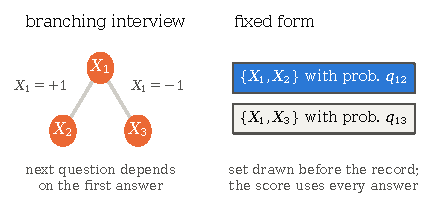
\includegraphics[width=\columnwidth]{figures/v13_protocols.pdf}
\caption{The worked example. A two-query branching interview asks $X_2$ after $X_1=+1$ and $X_3$ after $X_1=-1$. A fixed form commits to $\{1,2\}$ or $\{1,3\}$ before the record is seen and completes the tree's path only for half of the profiles.}
\label{fig:queries}
\end{figure}

\section{The Price of Pre-Commitment}\label{sec:gap}
\begin{theorem}[Exact simulation and the sharp gap]\label{thm:universal}
Let $1\le b\le m$ and $K_{m,b}=\min\{2^{b-1},\binom{m-1}{b-1}\}$.
\textup{(i)} Every protocol on $n$ branching records, with any estimator, is reproduced with the same law at every population by a fixed-form protocol on a random number of records with mean $K_{m,b}n$.
\textup{(ii)} Consequently, for every contrast of degree at most $b$ and with the constants $V$ and $W$ of Section~\ref{sec:general}, $V_{\rm fixed}\le K_{m,b}V_{\rm branch}$, and at every law $P$ of $(X,Y)$,
\begin{equation}
 W_{\rm branch}(P)\le W_{\rm fixed}(P)\le K_{m,b}\,W_{\rm branch}(P).\label{eq:universal}
\end{equation}
\textup{(iii)} The address contrast on $m=b-1+2^{b-1}$ coordinates has $V_{\rm fixed}/V_{\rm branch}=2^{b-1}$, and $W_{\rm fixed}(P)/W_{\rm branch}(P)=2^{b-1}$ at uniform profiles whenever the label agrees with the rule with a probability in $(0,1)$ that does not depend on the profile. With $m\le b^2$ there are examples with ratio at least $2^{b-b/(\lfloor\log_2 b\rfloor+1)-\lfloor\log_2 b\rfloor}$.
\end{theorem}

\begin{figure*}[t]
\centering
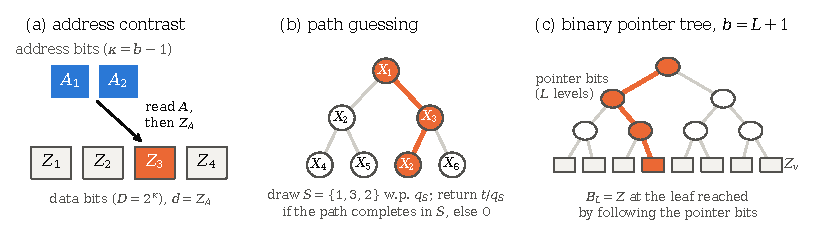
\includegraphics[width=\textwidth]{figures/v13_constructions.pdf}
\caption{The three constructions behind Theorems~\ref{thm:universal} and~\ref{thm:rounds}. (a) Address contrast: $\kappa=b-1$ address bits select one of $D=2^\kappa$ data bits; branching reads the address and then the selected bit, while any fixed set of $b$ coordinates explains at most a fraction $1/D$ of the target's variance under the uniform law. (b) Path guessing: a fixed form draws one of a tree's at most $2^{b-1}$ padded path sets and keeps the record when the path completes inside it. (c) Binary pointer tree: $L=b-1$ levels of pointer bits select a child and the target is the data bit at the reached leaf; a round that reads $a$ pointer bits raises the conditional probability of the most likely leaf by at most a factor $1+2a$ in expectation.}
\label{fig:constructions}
\end{figure*}

\begin{proof}
\emph{(i)} Remove repeated questions from a tree $\tau$ and pad every root-to-leaf path, by a fixed rule, with unused coordinates to exactly $b$ distinct ones. All path sets contain the root question, and the first $b-1$ answers determine the set, so the collection $\mathcal S_\tau$ of distinct path sets has at most $K_{m,b}$ elements. To simulate one record of $\tau$, draw one set of $\mathcal S_\tau$ uniformly and ask it as a form (Figure~\ref{fig:constructions}b). The answers reveal whether the drawn set is this record's own padded path set (follow the tree while its questions lie in the set), and for every profile exactly one set is; so the check succeeds with probability $1/|\mathcal S_\tau|$ whatever the record is. Accept a success with probability $|\mathcal S_\tau|/K_{m,b}$. An accepted record is then a draw from the population together with the transcript that $\tau$ would have produced, and the number of records used until acceptance is geometric with mean $K_{m,b}$ and independent of that transcript. The tree may depend on earlier transcripts, so the argument applies record by record to any protocol (Theorem~\ref{thm:simulation}). \emph{(ii)} For $V$, apply a near-optimal branching design to the records accepted from a fixed budget, whose number is binomial with success probability $1/K_{m,b}$. At a given $P$ an explicit score suffices: draw a tree of the branching design and one of its path sets, and return $c+|\mathcal S_\tau|(H-c)$ if the set is the record's own and $c$ otherwise, where $H$ is the tree's score and $c=\Delta(P)$. This score has the conditional mean of $H$ at every profile and at most $K_{m,b}$ times its variance (Appendix~\ref{app:population}). \emph{(iii)} Let $\kappa=b-1$ address bits select one of $D=2^\kappa$ data bits, $d(A,Z)=Z_A$ (Figure~\ref{fig:constructions}a). Branching computes $d$. Under the uniform law, a form $T$ with $s$ address bits and $w\ge1$ data bits has $s\le\kappa+1-w$ and explains the energy
\begin{equation}
 \|\E[d\mid X_T]\|_2^2=w\,2^{s-2\kappa}\le2^{-\kappa},\label{eq:addressinformation}
\end{equation}
because each of its data bits is consistent with a fraction $2^{-s}$ of the partial addresses and is then the selected bit with conditional probability $2^{-(\kappa-s)}$. The dual of Theorem~\ref{thm:char} with the uniform law and the witness $h=d$ compares $\|d\|_2^4=1$ with this energy, so $V_{\rm fixed}\ge D$. The same energy bounds the variance that a form explains when the label is a noisy copy of $d$ (Proposition~\ref{prop:labelnoise}), and products of address blocks give the example in polynomial dimension (Appendix~\ref{app:productaddress}).
\end{proof}
The gap requires that \emph{every} record obey the cap: under a mean budget of $b$ queries, asking all $m$ features with probability $b/m$ bounds the ratio by $m/b$ (Appendix~\ref{app:expectedproof}). For $m$ close to $b$ the extreme ratio is open (Proposition~\ref{prop:fourbit}).

\begin{theorem}[Rounds of adaptivity]\label{thm:rounds}
Let $K_r=\min\{2^{b-r},\binom{m-r}{b-r}\}$ and let $V_r$, $W_r(P)$ be the constants of $r$-round interviews.
\textup{(a)} Part \textup{(i)} of Theorem~\ref{thm:universal} holds for $r$-round interviews with $K_r$ in place of $K_{m,b}$; hence $V_r\le K_rV_{\rm branch}$ and $W_r(P)\le K_rW_{\rm branch}(P)$ at every $P$.
\textup{(b)} The binary pointer tree on $m=2^b-1$ coordinates has $V_{\rm branch}=1$ and $V_r\ge2^{b-1}/(1+2b/r)^{r}$ for $1\le r\le b$.
\textup{(c)} For $b\ge4$ a product of pointer trees on $m\le b^2$ coordinates has $V_{\rm branch}=1$ and $\log_2V_r\ge b-O(rb\log\log b/\log b)$.
\end{theorem}
For (a), follow the tree for $r-1$ rounds and guess the rest of the path in the last batch. For (b), a round that reads $a$ pointer bits raises the conditional probability of the most likely leaf by at most a factor $1+2a$ in expectation (Figure~\ref{fig:constructions}c); a potential argument makes this precise and extends to products (Appendix~\ref{app:roundshier}). On the pointer tree, a protocol within a polynomial factor of branching needs more than $0.37b-O(\log b)$ rounds. The product of part (c) loses $2^{b(1-o(1))}$ for every constant $r$ but is evaluated exactly in $\lfloor\log_2b\rfloor$ rounds; whether more than logarithmically many rounds can be necessary on $\mathrm{poly}(b)$ features is open. Appendix~\ref{app:pointerexact} computes the constants of the pointer tree at $b\in\{3,4\}$: two rounds lose $1.80$ and $3.33$, below the bounds $2$ and $4$ of part (a).

\section{Constants and Their Computation}\label{sec:general}\label{sec:population}
The simulation bounds the gap; the following constants measure it for a given contrast and population. A \emph{design} draws an interview $\iota$ with probability $q_\iota$ and scores its transcript with a table $g_\iota$; the score $Yg_\iota(\ell_\iota(X))/q_\iota$ is unbiased for $Yd(X)$ at every profile exactly when $\sum_\iota g_\iota(\ell_\iota(x))=d(x)$ for all $x$. Define the worst-case and population constants
\begin{align}
 V(d,\A)&=\inf_{q,g:\ \sum_\iota g_\iota=d}\ \max_{x\in\X}\sum_\iota\frac{g_\iota(\ell_\iota(x))^2}{q_\iota},\label{eq:unbiasedprogram}\\
 W_{\A}(P)&=\inf_{q,H:\,\E[H\mid X,Y]=t(X,Y)}\Var_{P,q}(H),\label{eq:mainW}
\end{align}
where $H$ is a score of the drawn interview's transcript and the label that may be tuned to $P$. Let $\sigma_P^2=\Var_P(t)$; for a depth-$b$ tree $\tau$ that computes $d$, with padded path sets $S_\tau(x)$, let $\rho_P^2=\max_{|T|=b}\Var_P(\E_P[t\mid X_T,Y])/\sigma_P^2$ be the largest share of the target's variance that one form explains, and $N_P(\tau)=(\sum_Sv_S^{1/2})^2$ with $v_S=\E_P[(t-\Delta)^2\mathbf 1\{S_\tau(X)=S\}]/\sigma_P^2$ the effective number of question sets the tree uses at $P$.

\begin{theorem}[Exact constants]\label{thm:char}\label{thm:bracket}
Let $\A$ be a finite menu on which $d$ is identifiable.
\textup{(a)} $nR_\A(d,n)\to V(d,\A)$; for every $\epsilon>0$ an iid design with an unbiased score has worst-case risk at most $(V+\epsilon)/n$ for every $n$, and the converse covers biased estimators, designs that adapt across records and interview choices that depend on the current label. Moreover $V(d,\A)=\sup_{\mu,h}\langle d,h\rangle_\mu^2/\max_{\iota\in\A}\|\E_\mu[h\mid\ell_\iota(X)]\|_\mu^2$ over positive profile laws $\mu$ and witnesses $h$.
\textup{(b)} At a full-support law $P$, $W_\A(P)/n$ is the local asymptotic minimax risk over arbitrary estimators from the capped records, for interviews drawn without the record's label; drawing them with the label can only lower the constant (Proposition~\ref{prop:labeldesign}).
\textup{(c)} If a depth-$b$ tree $\tau$ computes $d$ and $\sigma_P^2>0$, then $W_{\rm branch}(P)=\sigma_P^2$ and
\[
 \frac1{\rho_P^2}\ \le\ \frac{W_{\rm fixed}(P)}{W_{\rm branch}(P)}\ \le\ N_P(\tau)\ \le\ K_{m,b},
\]
with equality throughout for the address contrast under the uniform law. For every menu, constant $c$ and witness $h$ (with $0/0=0$), $W_\A(P)+(\Delta-c)^2\ge\E_P[(t-c)h]^2/\max_{\iota\in\A}\E_P[\E_P[h\mid\ell_\iota(X),Y]^2]$.
\end{theorem}
The ingredients are standard: minimax duality for linear functionals \citep{donoho1994,juditsky2009,polyanskiy2026}, information bounds over families of channels \citep{acharya2019,barnes2020}, and, for one menu, $c$-optimal design with the efficient augmented inverse-probability score under known coarsening \citep{elfving1952,pukelsheim1993,robins1994,tsiatis2006}. What is new is the comparison across menus and the exact optimization over the combinatorial menus of $r$-round and branching interviews. Ratios of $W$ are ratios of records needed when $n$ is large and each class uses its best design for $P$ (Appendices~\ref{app:B}, \ref{app:localminimax}, \ref{app:population}).

\begin{table}[t]
\centering
\caption{The constants of the paper. Ratios compare the best designs of two classes, each tuned to $P$.}
\label{tab:constants}
\footnotesize
\setlength{\tabcolsep}{2.5pt}
\begin{tabular}{lp{6.4cm}}
\toprule
$V(d,\A)$ & worst-case first-order constant, $\lim_n nR_\A(d,n)$\\
$W_\A(P)$ & smallest variance of a pointwise-unbiased design at $P$; local minimax risk times $n$\\
$K_{m,b}$ & $\min\{2^{b-1},\binom{m-1}{b-1}\}$: simulation factor; bound on the gap, attained if $m\ge b-1+2^{b-1}$\\
$\rho_P^2$, $N_P$ & share of $\Var_P(t)$ explained by the best form; effective number of the tree's question sets\\
$W^{(k)}_\A(P)$ & local minimax constant when the law lies in the log-linear model with interactions of order $\le k$\\
\bottomrule
\end{tabular}
\end{table}

\paragraph{Computing every protocol class.}
Pad every transcript to exactly $b$ coordinates, so that an interview is a partition of the cube into cells $\{x:x_T=a\}$ with $|T|=b$. Pointwise unbiasedness of the tables is then equivalent to matching the Fourier coefficients of $t$ of degree at most $b$, and \eqref{eq:mainW} over a list of interviews is a second-order cone program in the tables and the interview probabilities. Column generation solves a restricted master problem over a few interviews; for its dual witness, the most informative interview of any class $\A_r$ is found by dynamic programming over partial assignments (singleton batches give trees, one full batch gives forms). The witness certifies a lower bound through the last display of Theorem~\ref{thm:bracket}, and the master value is an upper bound. Pricing visits $O(\sum_{k\le b}\binom mk4^k)$ partial assignments per iteration and never touches the $2^m$ profiles (Appendix~\ref{app:engine}).

The unbiasedness identities hold at every profile, so a design fitted on reference data, or learned from a pilot of the evaluation itself, stays exactly unbiased when the reference is wrong; only its variance depends on it (Proposition~\ref{prop:selfcal}).

\section{What a Model Changes}\label{sec:model}
The constants so far assume nothing about the unasked features. Suppose instead that the law of $(X,Y)$ lies in a smooth parametric model with tangent space $\mathcal T$ at $P$. The records of an interview $\iota$ carry the information $J_\iota(h)=\E_P[\E_P[h\mid\ell_\iota(X),Y]^2]$ about a direction $h\in\mathcal T$, and the local asymptotic minimax constant of a menu \emph{within the model} is
\begin{equation}
 W^{\mathcal T}_\A(P)=\min_q\ \sup_{h\in\mathcal T}\ \frac{\langle t-\Delta(P),h\rangle_P^2}{\sum_\iota q_\iota J_\iota(h)},\label{eq:mainWT}
\end{equation}
with $0/0=0$. For the space of all mean-zero functions this is $W_\A(P)$; a model restricts the witness of Theorem~\ref{thm:bracket}(c) to $\mathcal T$. The value is a lower bound on the local minimax risk within the model, attained when the optimal design has nonsingular information (Proposition~\ref{prop:localmodel}), and the same solver computes it. Let $\mathcal M_k$ be the log-linear model with all interactions of order at most $k$ among the $m$ features and the label, with constants $W^{(k)}_\A$: $k=2$ is the pairwise model, and $k=m+1$ is saturated and returns $W_\A$. The submodel $\mathcal M_{\rm ci}\subset\mathcal M_2$ keeps only the interactions of each feature with the label.

\begin{theorem}[Adaptivity in a model]\label{thm:structured}
\textup{(a)} For every model, every law $P$ and $1\le r\le b$: $W^{\mathcal T}_r(P)\le K_r\,W^{\mathcal T}_{\rm branch}(P)$.
\textup{(b)} In the model $\mathcal M_{\rm ci}$ in which the features are independent given the label, at every law of the model and for every contrast: fixed forms, $r$-round and branching interviews have the same constant if the design may depend on the record's label, and $W^{\rm ci}_{\rm fixed}(P)\le2\,W^{\rm ci}_{\rm branch}(P)$ if it may not. At product laws with a balanced label the pairwise model has $W^{(2)}_{\rm fixed}=W^{(2)}_{\rm branch}$ for every contrast.
\textup{(c)} If the features and the label are independent under $P$, each taking both values with probability at least $\lambda$, then $W^{(k)}_{\rm fixed}(P)\le\min\{K_{m,b},\nu_k\}\,W^{(k)}_{\rm branch}(P)$ with $\nu_k=\sum_{j=1}^k\binom{b+1}j(\frac{1-\lambda}\lambda)^j$, at most $(b+1)^k$ at uniform laws; for $k\le b$ the bound holds up to a factor $1+\epsilon$ on a neighbourhood of $P$ in $\mathcal M_k$.
\textup{(d)} For the address contrast at the uniform law and $3\le k\le b+1$, the ratio $W^{(k)}_{\rm fixed}/W^{(k)}_{\rm branch}$ is at least $L_k(b)\ge\binom{b-1}{k-2}/b$; it is at least $(4/9+o(1))\,b$ for $k=3$ and equals $2^{b-1}$ for $k=b+1$.
\textup{(e)} For every $b\ge3$ and $\epsilon>0$ there are full-support laws in the pairwise model $\mathcal M_2$, on $b-1+3\cdot2^{b-1}$ features, at which $W^{(k)}_{\rm fixed}/W^{(k)}_{\rm branch}\ge(1-\epsilon)\,2^{b-1}/b$ for every $k\ge2$.
\end{theorem}
Part (a) is the simulation of Theorem~\ref{thm:universal}, which involves no model. Part (b) is the benign extreme, and it holds at rules of any accuracy: when the features are independent given the label, as in a naive-Bayes or latent-class model, a record informs the estimate only through \emph{which} coordinates it reveals; the constant of a design is $\Var(\E[t\mid Y])+\sum_yP(y)\sum_j(\hat d^{\,y}_j)^2/\pi_j(y)$, where $\pi_j(y)$ is the probability that feature $j$ is asked of a record with label $y$ and $\hat d^{\,y}_j$ is the degree-one coefficient of the rule in class $y$. Whatever inclusion probabilities a tree realizes, a label-dependent mixture of forms realizes as well, so adaptivity has no first-order value once the label may be used. Without the label a tree can use early answers as a proxy for it, and forms may need up to twice the records; an example with a noisy copy of the label among the features comes close to two (Appendix~\ref{app:structured}). Part (c) extends this to interactions of bounded order at laws without any dependence, by Cauchy--Schwarz over the low-order monomials inside a path set; part (d) locates the gap there for the contrast that attains $2^{b-1}$ without a model. Part (e) shows that parsimony alone is not enough: with a one-hot copy of the address and the products of its indicators with the data bits, tied by strong pairwise couplings as dummy-coded and derived items are, the target is a polynomial of degree two on a set of probability nearly one. What removes the gap is weak dependence among the features, not the order of the model. Between (b)--(c) and (e) no bound is proved: the neighbourhood in (c) has no explicit radius, and already at product laws with an unbalanced label the pairwise constants of forms and trees can differ (Appendix~\ref{app:structured}). Section~\ref{sec:experiments} computes the constants there.

\section{Experiments}\label{sec:experiments}
The experiments ask three questions about trained rules. \textbf{Q1:} what does pre-commitment cost when each class uses its best design? \textbf{Q2:} how much of that comparison is design optimization, and can the designs be found without knowing the population? \textbf{Q3:} what does a working model change, including when it is wrong? Every population $P$ is a held-out or target empirical law mixed with a uniform mass of $1\%$, which gives full support; the constants are oracle computations at these laws, certified by primal and dual bounds that agree to a relative error of at most $10^{-4}$ ($10^{-3}$ within a model) unless a bound is shown, and only the simulated audits involve sampling. Details are in Appendix~\ref{app:F}.

\begin{table*}[t]
\centering
\caption{BRFSS screening trees on twelve items (six runs per cap: two targets, three seeds): records needed relative to a branching interview that asks the tree\textquotesingle s own questions (which attains the full-information variance); medians over the six runs, range in brackets. \emph{Pre-committed forms without a model} (pointwise-unbiased scores): the optimal design at the target law; the design fitted on 20,000 source records; the design learned from a cross-fitted pilot of the audit itself with smoothed cell masses, all records charged ($N=4{,}000$; 1 when one form holds all the rule\textquotesingle s items); uniform randomization over all forms of the rule\textquotesingle s items and over the tree\textquotesingle s question paths, each with optimal tables. \emph{Two rounds}: the optimal two-round design (at $b=6$ the median includes certified upper bounds from feasible two-round designs for 4 runs, Table~\ref{tab:runs}). \emph{Bracket}: $[1/\rho_P^2,\ N_P]$ of Theorem~\ref{thm:bracket}. \emph{Within a model}: $W^{(k)}_{\rm fixed}/W^{(k)}_{\rm branch}$ at the order-$k$ log-linear fit of the target law.}
\label{tab:screening}
\footnotesize
\setlength{\tabcolsep}{2.4pt}
\begin{tabular}{r l r r r r r l l l}
\toprule
 & \multicolumn{5}{c}{pre-committed forms, no model} & two & bracket & \multicolumn{2}{c}{forms within a log-linear model} \\
\cmidrule(lr){2-6}\cmidrule(lr){9-10}
$b$ & optimal & reference & pilot & uniform, items & uniform, paths & rounds & $[1/\rho_P^2,N_P]$ & pairwise & three-way \\
\midrule
3 & 1.00 [1.00, 1.34] & 1.04 & -- & 1.00 & 1.03 & 1.00 & [1.00, 1.5] & 1.00 [1.00, 1.09] & 1.00 [1.00, 1.23] \\
4 & 1.49 [1.00, 1.75] & 1.57 & 1.62 & 2.30 & 1.80 & 1.00 & [1.18, 3.3] & 1.09 [1.00, 1.13] & 1.28 [1.00, 1.40] \\
5 & 1.35 [1.18, 1.54] & 1.42 & 1.53 & 2.04 & 1.72 & 1.00 & [1.08, 5.4] & 1.06 [1.02, 1.10] & 1.17 [1.08, 1.28] \\
6 & 1.58 [1.42, 1.98] & 1.68 & 1.93 & 4.18 & 2.30 & $\le$1.05 & [1.13, 10.5] & 1.07 [1.05, 1.13] & $\ge$1.18 [1.15, 1.33] \\
\bottomrule
\end{tabular}
\end{table*}


\paragraph{Q1: the cost of pre-commitment.}
A depth-$b$ screening tree asks at most $b$ questions per person, so a validation study under the same burden must respect the cap. We train class-balanced CART trees on twelve yes/no items of the CDC Diabetes Health Indicators, derived from the Behavioral Risk Factor Surveillance System (BRFSS; 253,680 respondents, target diabetes or prediabetes) \citep{cdcdiabetes2017}, and on twelve binarized thyroid items \citep{quinlan1986thyroid}, and validate them on a disjoint random half or on respondents of the other sex. On thyroid, and whenever a tree uses at most $b$ items, one form asks everything the rule needs and pre-commitment costs nothing. On BRFSS at caps four to six the best pre-committed design needs a median \nScreenBestLo--\nScreenBestHi{} times the respondents of branching (\nScreenRunLo--\nScreenRunHi{} over runs; Table~\ref{tab:screening}); label-dependent form probabilities lower this by at most \nLabelMax\%. \nRulesSentence{} A second round removes most of the gap: of the \nScreenGainN{} BRFSS diabetes trees with a gain, \nGainComputable{} are computed exactly by a two-round interview, \nGainExactNon{} more are within a factor \nScreenTwoMax{} of branching, and the remaining \nTwoBounded, at $b=6$, within \nTwoBoundMax{} (Figure~\ref{fig:rounds}a).

\begin{table}[t]
\centering
\caption{Further rules (depth-$b$ trees, $b\in\{4,5,6\}$, three seeds; BRFSS outcomes on 21 variables, Spambase on 57 features): records needed relative to branching by optimal and by uniformly drawn forms on the rule\textquotesingle s items, median [range] over the runs with a gain. Runs: with a gain / without (the rule uses at most $b$ items) / not computed (more than 13 items). Pairwise: $W^{(2)}_{\rm fixed}/W^{(2)}_{\rm branch}$ at the pairwise fit (rules with at most ten items). Details and bootstrap ranges: Table~\ref{tab:rules}.}
\label{tab:rulesmain}
\footnotesize
\setlength{\tabcolsep}{2pt}
\begin{tabular}{llllr}
\toprule
target & runs & optimal forms & uniform, items & pairw. \\
\midrule
heart disease & 7/0/2 & 1.57 [1.16, 2.38] & 3.2 [1.4, 16.8] & 1.16 \\
stroke & 7/0/2 & 1.37 [1.30, 1.79] & 2.1 [1.9, 3.7] & 1.12 \\
high blood pr. & 9/0/0 & 1.16 [1.07, 1.38] & 1.4 [1.3, 1.6] & 1.01 \\
diff. walking & 7/2/0 & 1.56 [1.24, 1.78] & 2.0 [1.4, 2.8] & 1.07 \\
spam & 8/0/1 & 1.97 [1.40, 2.13] & 4.8 [2.2, 8.4] & 1.18 \\
\bottomrule
\end{tabular}
\end{table}


\emph{Ensembles.} On WDBC, Spambase and Ionosphere \citep{wolberg1993,spambase1999,ionosphere1989}, an old and a new random forest of twenty depth-$b$ trees are trained on disjoint records with $m\in\{6,9,12\}$ median-binarized features; the contrast is the difference of the forests' predicted probabilities, which no single interview computes. At cap three the best pre-committed design needs a median \nCapThreeMed{} times the records of the best branching design (range \nCapThreeMin--\nCapThreeMax, Table~\ref{tab:capgrid}), and an optimal two-round design at most \nTwoForestRatioMax{} times in each of \nTwoForestN{} tasks. Here the cap costs more than pre-commitment: relative to complete records, the best fixed designs need \nCapFixLo--\nCapFixHi{} and the best branching designs \nCapBrLo--\nCapBrHi{} times as many. \nForestScaleSentence

\begin{figure}[t]
\centering
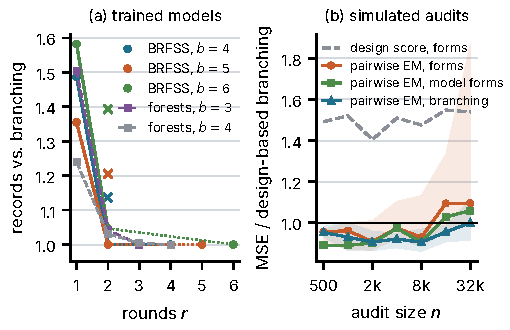
\includegraphics[width=\columnwidth]{figures/v20_rounds.pdf}
\caption{(a) Records needed relative to branching, without a model, as a function of the number of rounds ($r=1$: fixed forms; $r=b$: branching): optimal $r$-round designs for BRFSS screening trees (median over runs; at $b=6$, $r=2$ the median includes upper bounds) and forest updates (median over tasks); crosses mark the heuristic of following the root question. (b) Simulated audits: mean squared error relative to the design-based mean under branching, against the audit size, for the design-based form score and for the pairwise EM estimate on fitted forms, on forms optimized for the pairwise model, and on branching records (median over \nCurveTrees{} BRFSS trees; bands: quartiles).}
\label{fig:rounds}
\end{figure}

\paragraph{Q2: design optimization versus adaptivity.}
The ratios above compare optimized designs, and optimization accounts for much of what a naive comparison would credit to adaptivity. Uniform randomization over all forms of the rule's own items, with optimal tables, needs a median \nUitMedLo--\nUitMedHi{} times the records of branching by cap, and uniform matrix sampling over all twelve items \nUnifLo--\nUnifHi{} times; uniform randomization over the tree's question paths needs a median \nUpsOverMed\% more than the optimized forms. The optimized designs do not require knowing the population. Forms fitted on 20,000 source records need a median \nFitMed\% more than the oracle and stay exactly unbiased. With no reference, the design is learned from a pilot of the audit itself, which must be charged: with a quarter of $N=4{,}000$ records as a cross-fitted pilot on the tree's paths and cell masses smoothed by a pairwise fit, the all-in price is a median \nPilotAllLo--\nPilotAllHi\% above the oracle of the same run (\nPilotEmpLo--\nPilotEmpHi\% with unsmoothed frequencies; Table~\ref{tab:pilotsmooth}). The bracket of Theorem~\ref{thm:bracket} is loose on these rules (Table~\ref{tab:screening}), so the solver is needed.

\begin{table}[t]
\centering
\caption{Forest updates of depth $b$ under cap $b$ (WDBC, Spambase, Ionosphere; binding tasks). Fixed/branch: exact $W_{\rm fixed}/W_{\rm branch}$, median [minimum, maximum]. Fit: median excess of the ratio realized by designs optimized on training records over the exact ratio of the same task ($^\dagger$the 15 tasks with $m=12$). Own: share of the log-gap captured when branching may use only the forests\textquotesingle{} own trees. Two: exact optimal two-round design, $W_2/W_{\rm branch}$ ($^\ddagger$five splits per cell: 45 and 15 tasks; at $b=2$ two rounds are branching). Cap: $W_{\rm fixed}$ and $W_{\rm branch}$ relative to the full-information variance.}
\label{tab:capgrid}
\footnotesize
\setlength{\tabcolsep}{2.6pt}
\begin{tabular}{rrlrrrrr}
\toprule
 & & & & & & \multicolumn{2}{c}{Cap: /full} \\
$b$ & tasks & Fixed/branch & Fit & Own & Two & fixed & branch \\
\midrule
2 & 45 & 1.31 [1.12, 1.49] & +1\% & 49\% & 1 & 4.1 & 3.3 \\
3 & 180 & 1.51 [1.14, 1.85] & +2\%$^\dagger$ & 17\% & 1.04$^\ddagger$ & 3.5 & 2.3 \\
4 & 15 & 1.24 [1.13, 1.35] & +3\% & 26\% & 1.03$^\ddagger$ & 1.4 & 1.1 \\
\bottomrule
\end{tabular}
\end{table}


\paragraph{Q3: what a working model changes.}
\emph{Constants when the model holds.} \nCiSentence{} With interactions among the features the constants are computed: we refit each target law by the pairwise and the three-way log-linear model on the label and the rule's items and solve for forms and for depth-$b$ trees at the fit (Table~\ref{tab:model}). Under the pairwise model forms need \nModelTwoLo--\nModelTwoHi{} times the records of the best branching design on the diabetes trees (\nModelAllLo--\nModelAllHi{} over all rules with at most ten items), where the design-based ratio at the same laws is \nModelDesignLo--\nModelDesignHi; under the three-way model the ratio is \nModelThreeLo--\nModelThreeHi. On synthetic laws the solver reproduces both ends of the theorem: at pairwise fits of noisy address populations the pairwise ratio stays at \nDepFitTwoMax, whereas along the strongly coupled laws of part (e) it rises from one to \nDepRatioLast{} at $b=3$ (Table~\ref{tab:dependence}).

\emph{When the model is wrong.} \nMisspecSentence

\emph{Simulated audits.} \nAuditParagraph

\paragraph{Further checks.}
An optimized design is tailored to one rule: scoring another tree on its records needs \nReuseMin{} to \nReuseMax{} times the records of branching, whereas one design shared by three known trees costs each a median \nJointPenMed\% more than its own optimum (Appendix~\ref{app:reuse}). Imputation from complete records of another population beats every capped design when the conditional law of the unasked items transports; in \nImpBadN{} of the eight shift settings (four pre-specified shifts at two caps) it is biased, and multiple imputation covers \nMiCovLo--\nMiCovHi{} (Table~\ref{tab:shift}).


\section{Related Work}\label{sec:related}
\paragraph{Adaptivity in query and decision models.} Within-input adaptivity is classical in decision-tree and property-testing complexity, with round hierarchies for testers and oracle evaluation \citep{canonne2018,li2026regex} and pointer chasing in communication \citep{nisan1993}; that a $q$-query adaptive procedure is simulated by $2^q$ non-adaptive queries to the same input is folklore there, and Theorem~\ref{thm:universal}(i) is that conversion carried out across records under a cap of $b$ queries each, with an acceptance step that makes the simulation exact in law and gives the constant $K_{m,b}$; the locally bounded model of \citet{adar2024}, with its exponential separation from non-adaptive testers \citep{goldreich2022,chakraborty2023}, is the testing counterpart of our branching class. Adaptivity gaps are also studied in stochastic optimization \citep{dean2008,golovin2011}, batched bandits \citep{perchet2016,gao2019} and adaptive sensing \citep{ariascastro2013}. None of these gives the price in records, for estimation, of fixing a record's questions in advance, its exact constant, or its behaviour under a model.

\paragraph{Information-constrained estimation.} Estimation under communication and local-privacy constraints fixes a per-sample channel family \citep{acharya2019,barnes2020,acharya2022tit,lau2026}, and pointer chasing separates rounds of interaction in local privacy \citep{joseph2019,joseph2020}. Ours is a noiseless analogue with exact constants.

\paragraph{Optimal design and missing data by design.} For one menu our programs are $c$-optimal design and our solver a vertex-direction method \citep{elfving1952,fedorov1972,wynn1970,pukelsheim1993,sagnol2011}; minimax pairs of a design and a design-unbiased estimator are classical for fully observed units \citep{stenger1979,gabler1990,aronow2026}. Split questionnaires and matrix sampling assign fixed forms \citep{raghunathan1995,graham2006,thomas2006,chipperfield2009,rhemtulla2012}, which have been optimized under a model from a pilot or an earlier wave \citep{adiguzel2008,jang2022}, and known-coarsening theory gives the efficient estimator for a fixed mechanism \citep{robins1994,tsiatis2006}. Adaptive matrix sampling \citep{gonzalez2008}, responsive design \citep{groves2006}, two-phase designs \citep{reilly1995,gilbert2014,mcisaac2015,tao2020,chen2020,chen2022} and multistage adaptive tests \citep{yamamoto2018,fink2024} are two-round interviews in our sense. These lines optimize one protocol within one design space; we compare the spaces.

\paragraph{Evaluation and acquisition in ML.} Restricted-focus-of-attention learning chooses a few attributes of each example before seeing it, our fixed-form class \citep{bendavid1998}, and budgeted learning fits predictors from such views \citep{cesa2011,hazan2012,lizotte2003,kapoor2005}. Active testing and prediction-powered inference allocate labels \citep{kossen2021,zrnic2024,angelopoulos2023}, the reverse of our cost structure; active feature acquisition chooses features for individual predictions \citep{trapeznikov2013,nan2017,covert2023,vonkleist2025}.

\section{Discussion and Limitations}\label{sec:discussion}
Within-record adaptivity is worth at most $2^{b-1}$ in records, for every task, model and population, sharply without a model, and it accrues round by round. A model with features independent given the label removes the gap, up to a factor two if forms are drawn without the label, and a pairwise model removes little of it when strong couplings encode the rule's structure. \nDiscussionSentence

\emph{In practice.} \nPracticeSentence

\emph{Scope.} For a single screening tree the adaptive optimum is the rule itself, so the comparison prices paper forms and panels ordered in one batch against computer-assisted administration of the rule; for ensembles the cap costs more than pre-commitment (Table~\ref{tab:capgrid}). The target is one known low-degree functional fixed before collection: records collected for one rule can be nearly useless for another (Appendix~\ref{app:reuse}), and thresholded ensembles exceed small caps. Labels are free and always observed; if the cap can be relaxed and labels are expensive, complete records can be cheaper (Appendix~\ref{app:costchoice}). Answers are assumed not to depend on question order or mode; \nOrderSentence{}

\emph{What the constants mean.} Ratios of $W$ compare designs tuned to the population in the limit of many records per cell, and the finite-sample bracket of Theorem~\ref{thm:finite} carries a factor of 104. The model-based constants hold when the model does. The populations are unweighted, smoothed empirical laws; no audit was run in the field. Pricing visits on the order of $\binom mb4^b$ partial assignments per iteration: adaptive classes were solved for $m\le12$, $b\le6$ and for $m=20$ at $b=3$ only.

\section*{Impact Statement}
Shorter adaptive questionnaires and test sequences can reduce respondent and patient burden. Branching exposes people to different questions; order effects, selective nonresponse and subgroup-specific burdens can bias estimates or hide unequal outcomes, and population-average gains do not imply subgroup gains, so deployments should monitor both.

\bibliography{refs}
\bibliographystyle{icml2026}
\clearpage
\onecolumn
\raggedbottom
\appendix
\counterwithin{theorem}{section}
\counterwithin{equation}{section}
\section{Guide, Notation and a Worked Example}\label{app:notation}
\paragraph{Guide.}
Appendix~\ref{app:B} proves Theorem~\ref{thm:char}; Appendix~\ref{app:C} proves Theorem~\ref{thm:universal} and its extensions to finite samples, larger alphabets, polynomial dimension and mean budgets; Appendix~\ref{app:D} proves Theorem~\ref{thm:rounds}, including the product construction in polynomial dimension, and reports the round constants of the binary pointer tree at small caps; Appendix~\ref{app:E} proves the population statements (Theorems~\ref{thm:universal}(ii), \ref{thm:rounds}(a) and~\ref{thm:bracket}, Propositions~\ref{prop:labeldesign}, \ref{prop:labelnoise}, \ref{prop:upper} and~\ref{prop:selfcal}), the statements about models (Theorem~\ref{thm:structured}, Proposition~\ref{prop:localmodel}; Appendix~\ref{app:structured}), and describes the solver and the form program; Appendix~\ref{app:F} gives every experimental detail; Appendix~\ref{app:metrics} extends the estimator to other proper scores; Appendix~\ref{app:repro} describes code and checks.

\paragraph{Notation.}
\begin{center}\small
\begin{tabular}{lp{10.5cm}}
\toprule
Symbol & Meaning\\
\midrule
$d=p_1-p_0$, $t(x,y)=yd(x)$ & Contrast of the two frozen rules and the per-record target; $\Delta(P)=\E_P[t]$\\
$\iota$, $\ell_\iota(x)$, $\A$ & Interview, its transcript, and a finite menu of interviews\\
$\A_r(b)$ & $r$-round interviews with at most $b$ queries; $\A_1$ fixed forms, $\A_b$ branching trees\\
$q_\iota$, $g_\iota$ & Interview probabilities and transcript score tables of a design\\
$V(d,\A)$, $V_r$ & Worst-case first-order constant \eqref{eq:unbiasedprogram}; its value on $\A_r(b)$\\
$\Phi_n(d,\A)$ & Finite-sample program \eqref{eq:program}, within a factor 104 of the minimax risk (Theorem~\ref{thm:finite})\\
$W_\A(P)$, $M_\A(P)$ & Smallest variance and second moment of a pointwise-unbiased design at $P$; $M=W+\Delta^2$\\
$\sigma_P^2$, $\rho_P^2$ & $\Var_P(t)$; largest share of it explained by one form, $\max_{|T|=b}\Var_P(\E_P[t\mid X_T,Y])/\sigma_P^2$\\
$N_P(\tau)$ & R\'enyi-$1/2$ effective number of path sets, from the centered weights $v_S=\E_P[(t-\Delta)^2\mathbf 1\{S_\tau=S\}]/\sigma_P^2$\\
$W_{\rm PS}(P)$ & Optimum over the padded path sets of a tree computing $d$ (Proposition~\ref{prop:upper})\\
$W^{\rm lab}_\A(P)$ & Optimum when interview probabilities may depend on the label (Proposition~\ref{prop:labeldesign})\\
$\mathcal T$, $J_\iota(h)$, $W^{\mathcal T}_\A(P)$ & Tangent space of a model at $P$, information of interview $\iota$ about $h\in\mathcal T$, and the local minimax constant within the model \eqref{eq:WT}\\
$\mathcal M_k$, $W^{(k)}_\A(P)$ & Log-linear model with interactions of order at most $k$ among the features and the label, and its constant\\
$K_{m,b}$ & $\min\{2^{b-1},\binom{m-1}{b-1}\}$\\
$\kappa$, $D=2^\kappa$ & Address bits and data bits of the address contrast; $L$ levels of the binary pointer tree\\
$\U$ & Uniform law on the profile cube\\
$B$; $n_1$ & Larger hard cap in the mixed-budget result; pilot size in Proposition~\ref{prop:selfcal}\\
\bottomrule
\end{tabular}
\end{center}

\paragraph{The worked example in full.}
Let $m=3$, $b=2$ and $d(x)=[(1+x_1)x_2+(1-x_1)x_3]/2$, and let $P$ have uniform profiles and an independent uniform label, so that $\Delta(P)=0$ and $\sigma_P^2=\E[d^2]=1$. The tree asks $x_1$ and then $x_2$ or $x_3$; it computes $d$, so $V_{\rm branch}=1$ and $W_{\rm branch}(P)=1$. The Fourier expansion is $d=\tfrac12x_2+\tfrac12x_3+\tfrac12x_1x_2-\tfrac12x_1x_3$. Each coefficient carries a quarter of the variance, and every form of size two contains exactly two of the four sets: $\{1,2\}$ captures $x_2$ and $x_1x_2$, $\{1,3\}$ captures $x_3$ and $x_1x_3$, and $\{2,3\}$ captures $x_2$ and $x_3$. Hence $\rho_P^2=1/2$ and $W_{\rm fixed}(P)\ge2$. The two padded path sets $\{1,2\}$ and $\{1,3\}$ each carry weight $v_S=1/2$, so $N_P=(2\cdot2^{-1/2})^2=2$, and drawing either form with probability $1/2$ and returning $2Yx_2\mathbf1\{x_1=1\}$ or $2Yx_3\mathbf1\{x_1=-1\}$ attains second moment $2$ at every profile. Thus $V_{\rm fixed}=W_{\rm fixed}(P)=2=K_{3,2}$, both ends of Theorem~\ref{thm:bracket} coincide, and the optimized path-set design of Proposition~\ref{prop:upper} equals the optimum. If instead the label agrees with $d(X)$ with probability $0.9$, then $t=\pm1$ with $\Delta=0.8$ and $\sigma_P^2=0.36$; the centered weights are again $1/2$ each, so $N_P=2$ and the fixed design that returns $0.8+2(t-0.8)$ on a completed path and $0.8$ otherwise has variance $2\sigma_P^2$, whereas the uncentered path-guessing score has variance $2-0.64=1.36=3.78\,\sigma_P^2$. Section~\ref{sec:gap} generalizes the example to $\kappa$ address bits.

\section{Identification and the Exact Characterization}\label{app:B}
\subsection{General Statistical Guarantees}\label{app:generalstatements}
For a design distribution $q$ on $\A$ and a table $g_\iota$ on each transcript alphabet, abbreviate $g_\iota(x)=g_\iota(\ell_\iota(x))$ and $s_g(x)=\sum_\iota g_\iota(x)$. Define
\begin{align}
 B_n(q,g;x)&=(d(x)-s_g(x))^2+
              \frac1n\sum_{\iota\in\A}\frac{g_\iota(x)^2}{q_\iota},\nonumber\\
 \Phi_n(d,\A)&=\inf_{q,g}\ \max_{x\in\X}B_n(q,g;x).
 \label{eq:program}
\end{align}
A design of mass zero may only have a zero table, in which case its contribution is zero. The first term permits a controlled approximation of the update. The second accounts for observing only one of the tables per respondent.

\begin{theorem}[Finite-sample risk]\label{thm:finite}
For every finite $\X,\A$, every contrast $d$ and every $n\ge1$,
\[
       \Phi_n(d,\A)/104 \ \le\ R_\A(d,n)\ \le\ \Phi_n(d,\A).
\]
The upper bound uses one iid design and the mean of $Yg_\iota(\ell_\iota(X))/q_\iota$. The lower bound allows the choice of interview to depend on all previous records.
\end{theorem}

The constant 104 is conservative. This is a convex quadratic-perspective program with a finite second-order cone formulation. Its size depends on enumerated profiles and interviews; Section~\ref{sec:pathdesign} instead uses a compact tree representation for a restricted menu.

\begin{samepage}
\begin{theorem}[Exact leading variance]\label{thm:asym}
If $d\in\Hh_{\A}$, then $\lim_{n\to\infty}nR_\A(d,n)=V(d,\A)$ for fixed $d,\X,\A$. An iid design and an unbiased score give risk at most $V(d,\A)/n$ for every $n$.
\end{theorem}
\end{samepage}

An optimal iid design already achieves the first-order worst-case coefficient. The lower bound even permits observing the current label before selecting an interview, so early labels do not improve this coefficient either. Within-person branching changes the available observation maps themselves. Population-specific performance can still benefit from learning a design from previous people.

\paragraph{Why the characterization holds.}
Conditioning on the complete record bounds the score mean's squared bias and variance by \eqref{eq:program}. For the converse, put $\Pi_\iota h=\E_\mu[h\mid\ell_\iota(X)]$ and $J_\mu(h)=\max_\iota\|\Pi_\iota h\|_{2,\mu}^2$. Convex duality gives
\begin{equation}
 \Phi_n(d,\A)=\sup_{\mu,h}
 \frac{\ip{d}{h}^2}{\|h\|_{2,\mu}^2+nJ_\mu(h)}.\label{eq:dual}
\end{equation}
A witness perturbs the conditional label mean. Its numerator measures the change in the target, while $J_\mu(h)$ limits information from each interview. A change of measure and the KL chain rule handle sequential choices; a local van Trees argument gives the exact coefficient. Appendix~\ref{app:general} gives the duality and information proofs. These are established tools for linear-functional estimation; the sharp comparison of query menus is the main result.

\subsubsection{An Exact One-Feature Example}
For an additive contrast $d(x)=c_0+\sum_{j=1}^m c_j x_j$ on the unrestricted sign cube, put $M=\sum_{j=0}^m |c_j|=\|d\|_\infty$.
\begin{proposition}\label{prop:add}
For every $n\ge1$ the minimax risk is $M^2/(1+\sqrt n)^2$ both with full profiles and with at most one feature query.
\end{proposition}
Choose $j$ with probability $|c_j|/M$, interpret $x_0=1$, and return the sign $Y\sgn(c_j)x_j$. Its mean is $\Delta/M$. Estimating that mean reduces to a binomial problem. A population concentrated at an extremal profile gives the same binomial problem to an evaluator who sees all features (Appendix~\ref{app:sign}). Equality concerns worst-case populations. The best length at equal monetary cost can differ for particular populations.



\subsection{Identifiability and Irreducible Error}\label{app:id}
Let $L_\iota$ lift a transcript table to $\mathbb R^{\X}$, so $(L_\iota u)(x)=u(\ell_\iota(x))$. The space $\Hh_\A=\sum_\iota\mathrm{im}(L_\iota)$ is closed. Put $\delta=\inf_{v\in\Hh_\A}\|d-v\|_\infty$. In fact $\lim_{n\to\infty} R_\A(d,n)=\delta^2$. For the upper bound choose an approximant $v$ attaining $\delta$, decompose $v=\sum_\iota L_\iota g_\iota$, and give every used interview positive probability. The mean score is uniformly within $\delta$ of $\Delta$, and its variance tends to zero uniformly over $P$ since all alphabets are finite.

If $\delta>0$, finite-dimensional norm duality gives a signed vector $w$ of $\ell_1$ norm one annihilating $\Hh_\A$ with $\sum_xw(x)d(x)=\delta$. This follows by separating $d$ from the open $\ell_\infty$ ball of radius $\delta$ around that subspace, or by duality of the linear program for uniform approximation. In particular $\sum_{x:\ell_\iota(x)=u} w(x)=0$ for every $\iota,u$. Give $X$ the law $|w|$, and in the two populations set $Y=\pm\sgn w(X)$. For each $y$, each transcript cell has identical joint probability with $Y=y$ in the two populations. This remains true if $y$ determines which interview is used. Sequentially conditioning on past records gives identical transcript laws for $n$ interviews while the gains are $\pm\delta$. The average of the two squared risks is at least $\delta^2$. The same reasoning gives necessity in the identification criterion.

For a binary coordinate mask $T$ its cells span all characters $\chi_S$ with $S\subseteq T$ and no other characters, by the uniqueness of the multilinear expansion. A decision-tree leaf indicator is a product of up to $b$ factors $(1\pm x_i)/2$. Conversely the fixed query of $S$ recovers $\chi_S$ for every $|S|\le b$. This proves the common identification threshold.

\subsection{The General Minimax Characterization}\label{app:general}
Let $\|\cdot\|_\mu$ denote the norm in $L^2(\mu)$, identifying functions equal on the support of $\mu$. All objects below are finite-dimensional. We can take $q$ strictly positive when computing infima. If a feasible boundary design has $q_\iota=0$, its table is zero; mixing $q$ with a positive design and taking the mixture coefficient to zero recovers the same objective. Empty transcript cells can be discarded.

\subsubsection{The Dual Form}
For a fixed $\mu$ define, on the span of the transcript subspaces of $L^2(\mu)$,
\[
 N_\mu(v)=\inf_{\sum_\iota f_\iota=v}\sum_\iota\|f_\iota\|_\mu,\qquad f_\iota\in\mathrm{im}(L_\iota);
\]
extend it by $+\infty$ outside that span. The dual seminorm on the full space is $N_\mu^*(h)=\max_\iota\|\Pi_\iota h\|_\mu$. Indeed $|\ip{h}{\sum_\iota f_\iota}|\le\max_\iota\|\Pi_\iota h\|_\mu\sum_\iota\|f_\iota\|_\mu$, and a single normalized projection onto a maximizing subspace attains the bound. The closed unit ball of $N_\mu$ is the image of a compact product-space unit ball, so its squared norm is lower semicontinuous.

Maximizing over profiles in \eqref{eq:program} is equivalent to maximizing its expectation over all $\mu$. The objective is continuous affine in $\mu$ on the compact probability simplex and continuous convex in $(q,g)$ for positive $q$. Sion's minimax theorem exchanges maximum and infimum \citep{sion1958}. For fixed tables, Cauchy--Schwarz and $q_\iota\propto\|L_\iota g_\iota\|_\mu$ give
\[
 \inf_q \sum_\iota\|L_\iota g_\iota\|_\mu^2/q_\iota
      =\Big(\sum_\iota\|L_\iota g_\iota\|_\mu\Big)^2
\]
with zeros handled by limits. Thus at fixed $\mu$ the inner value is $\inf_v \{\|d-v\|_\mu^2+N_\mu(v)^2/n\}$. By finite-dimensional Fenchel duality this equals
\[
 \sup_h\{2\ip{d}{h}-\|h\|_\mu^2-nN_\mu^*(h)^2\}.
\]
To verify the factors, set $F(v)=\|d-v\|_\mu^2$ and $G(v)=N_\mu(v)^2/n$. Their conjugates satisfy
\[
 F^*(u)=\langle u,d\rangle_\mu+\|u\|_\mu^2/4,
 \qquad G^*(u)=nN_\mu^*(u)^2/4.
\]
Fenchel duality gives $\inf_v(F+G)(v)=\sup_u[-F^*(-u)-G^*(u)]$; substituting $u=2h$ gives the displayed expression. There is no duality gap because the first squared norm is finite and continuous everywhere and the second is proper convex. Optimizing over the scale of $h$ proves \eqref{eq:dual}.

\paragraph{Relation to fixed-channel constants.}
For a prescribed iid observation kernel, the $\chi^2$-modulus bound of \citet{polyanskiy2026} brackets MSE between the squared modulus divided by $(1+\sqrt e)^2$ and the squared modulus, under its stated assumptions. \citet{juditsky2009} instead formulate their main comparison using a confidence-level error criterion. Neither modulus is the joint-design objective in \eqref{eq:program}. Our factor 104 is a conservative conversion for that objective under sequential interview choice, not an improvement on fixed-channel constants. The additional argument is a witness whose information is bounded simultaneously for every eligible interview, including the two choices selected by the current label.

\subsubsection{Finite-Sample Converse}
The upper bound in Theorem~\ref{thm:finite} follows from the conditional-score calculation in Section~\ref{sec:general}. For the lower bound fix $\mu,h$ and normalize $\|h\|_\mu^2+nJ_\mu(h)=1$. Write $C_\mu=1+\E_\mu|h|\le2$ and set
\[
 \nu(x)=\mu(x)(1+|h(x)|)/C_\mu,\qquad
 u(x)=\mu(x)h(x)/\nu(x)
\]
on the support of $\mu$, with $u=0$ elsewhere. We have $\|u\|_\infty\le2$, $\nu\ge\mu/2$, and $\E_\nu[du]=\ip{d}{h}$. For every partition into transcript cells $C$,
\[
 \sum_C \nu(C)\,\E_\nu[u\mid C]^2
  =\sum_{C:\nu(C)>0}\frac{\big(\sum_{x\in C}\mu(x)h(x)\big)^2}{\nu(C)}
  \le 2\|\Pi_\iota h\|_\mu^2 .
\]
For $\vartheta=1/5$ define $P_\pm(x,y)=\nu(x)(1\pm \vartheta y u(x))/2$. Their gains are $\pm \vartheta\ip{d}{h}$. Condition on past interviews and on independent random coins. Under the null law with $X\sim\nu$ and $Y$ fair and independent, the probability $p_0(z)$ of a leaf $z=(y,C)$ changes to $p_\pm(z)=p_0(z)(1\pm \vartheta s_z)$ with $s_z=y\E_\nu[u\mid C]$. If the label selects interview $\iota_y$, the null second moment is
\[
 \E_0s_z^2=\frac12\sum_{y\in\{-1,1\}}\sum_{C\in \iota_y}
       \nu(C)\E_\nu[u\mid C]^2
 \le\frac12\sum_y 2\|\Pi_{\iota_y}h\|_\mu^2\le2J_\mu(h).
\]
Also $|s_z|\le2$. The conditional divergence satisfies
\[
 \KL(p_+\Vert p_-)\le\chi^2(p_+\Vert p_-)
    \le \frac{4\vartheta^2}{1-2\vartheta}\E_0 s_z^2
    \le \frac{8\vartheta^2}{1-2\vartheta}J_\mu(h).
\]
The bound is uniform in the realized past. Independent protocol randomness can be revealed at the start, then discarded by data processing. The KL chain rule bounds the divergence of the two full experiments by $8/15$. Pinsker's inequality bounds their total variation by $2/\sqrt{15}$. Classifying an estimate by the nearer of the two parameter values yields worst-case squared risk at least $\vartheta^2\ip{d}{h}^2(1-2/\sqrt{15})/2\ge\ip{d}{h}^2/104$. Taking the supremum in \eqref{eq:dual} proves Theorem~\ref{thm:finite}. The numerical inequality is equivalent to $15\cdot27^2>104^2$. The losses come from the change of measure, the KL-to-total-variation conversion, and testing two alternatives. The same calculation applies when the current label cannot select the form; this constant is not caused solely by label-dependent selection.

\subsubsection{Exact First-Order Constant}
Assume $d\in\Hh_\A$. Apply the same minimax exchange to \eqref{eq:unbiasedprogram}, retaining the affine pointwise constraint $s_g=d$. For strictly positive $\mu$ the pointwise constraint is equivalent to equality in $L^2(\mu)$, so the fixed-$\mu$ optimum is $N_\mu(d)^2$. Restricting the supremum to such $\mu$ preserves its value. Indeed mixing any $\mu$ with $\epsilon$ times a positive law gives an inner objective at least $(1-\epsilon)$ times the original one for every feasible design. By duality,
\begin{equation}
 V(d,\A)=\sup_{\mu>0,\,h:\,J_\mu(h)>0}
                \frac{\ip{d}{h}^2}{J_\mu(h)}.\label{eq:vdual}
\end{equation}
The zero contrast has value zero. Equation~\eqref{eq:dual} and \eqref{eq:vdual} also give $n\Phi_n\to V$: the upper bound is $V$ by a zero-residual design, and every fixed witness in \eqref{eq:vdual} gives the matching lower limit.

For a lower bound on $nR_\A$, fix positive $\mu,h$ and set $P_\theta(x,y)=\mu(x)(1+\theta y h(x))/2$, $|\theta|\le\eta<1/\|h\|_\infty$. Then $\Delta(P_\theta)=\theta c$, with $c=\ip{d}{h}$. For each history and deterministic choice of interviews the conditional leaf law has the form $p_\theta(z)=p_0(z)(1+\theta s_z)$. At the null $\E_0s_z^2\le J_\mu(h)$ and $|s_z|\le\|h\|_\infty$. Its Fisher information at $\theta$ is therefore at most $J_\mu(h)/(1-\eta\|h\|_\infty)$. Conditional likelihood scores are martingale differences, so the full information is bounded by $n$ times this quantity, including for a randomized protocol with its independent seed revealed.

Use a smooth prior $\pi_\eta$ on $[-\eta,\eta]$ vanishing at both endpoints with finite information $I(\pi_\eta)$, for example $\eta^{-1}\cos^2(\pi \theta/(2\eta))$. Integration by parts in the joint data--parameter law gives $\E[(\widehat\Delta-\theta c)\partial_\theta\log(p_\theta\pi_\eta)]=c$. Cauchy--Schwarz gives the van Trees inequality \citep{gill1995}, here a lower bound of
\[
     \frac{c^2}{nJ_\mu(h)/(1-\eta\|h\|_\infty)+I(\pi_\eta)}
\]
on the prior risk, and hence on worst-case risk. First take $n\to\infty$ after multiplying by $n$, then $\eta\downarrow0$, then optimize \eqref{eq:vdual}. The means of the unbiased scores in \eqref{eq:unbiasedprogram} give the opposite inequality for every $n$, proving Theorem~\ref{thm:asym}.

\subsubsection{When the Constant Is Attained in the Unbiased Class}
For a fixed positive design law $q$ such that the eligible cells span $d$, the analogous program $V_q(d)$ fixes $q$ in \eqref{eq:unbiasedprogram}. Its value divided by $n$ is exactly the worst-case minimax MSE among globally unbiased estimators with iid design $q$. To see the lower bound, choose $X\sim\mu$ of full support and an independent fair label. For a symmetric unbiased statistic $U_n$ of observations $O_i=(\iota_i,\ell_{\iota_i},Y_i)$ put $H(O_1)=\E[U_n\mid O_1]-\E U_n$. Orthogonality of the one-observation projections gives $\Var U_n\ge n\E H^2$. Perturbing the joint law to $\mu(x)(1+t y h(x))/2$ and differentiating unbiasedness gives $\ip{d}{h}=n\E[H(O_1)Y_1h(X_1)]$ for all $h$. Thus $d=\sum_\iota L_\iota g_\iota$ with $g_\iota(\ell)=nq_\iota\E[YH\mid \iota,\ell]$. Jensen bounds $\Var U_n$ below by $n^{-1}\inf_{s_g=d}\sum_\iota\|L_\iota g_\iota\|_\mu^2/q_\iota$. Taking the supremum over full-support $\mu$ and exchanging extrema as above gives the claim. Symmetrization costs no risk with iid records.



\section{The Sharp Gap and Its Extensions}\label{app:C}
\subsection{The Sharp Universal Gap}\label{app:universal}
We prove Theorem~\ref{thm:universal} and the program comparison
\begin{equation}
 \Phi_n(d,\A_{\rm fixed}(b))
 \le \Phi_{n/K_{m,b}}(d,\A_{\rm branch}(b)).
 \label{eq:programsimulation}
\end{equation}
Here the program is defined for any positive real sample-size argument.
All scores in the construction below depend only on the queried feature values; the estimator subsequently multiplies them by $Y$. Theorems~\ref{thm:finite} and~\ref{thm:asym} already compare these constructions with the larger class of history-dependent protocols, including branching choices based on the current label.

\subsubsection{Simulating One Tree without Branching}
Let $\tau$ be a deterministic tree of depth at most $b$ on $m\ge b$ coordinates, and let $H_\tau(x)$ be a score constant on each of its leaves. A repeated query on a path can be removed because its answer is already known. At every leaf with fewer than $b$ distinct queries, append unused coordinates in increasing index order until the path length is $b$. Copy the original score to all descendants. For a tree with no queries, start with any coordinate. The padded tree has exactly $b$ distinct queries on every path and the same score at every $x$.

Let $S_\tau(x)$ be its realized set of coordinates and let $\mathcal S_\tau$ be the collection of distinct such sets. Put $L_\tau=|\mathcal S_\tau|$. All sets contain the root, giving $L_\tau\le\binom{m-1}{b-1}$. The first $b-1$ answers fix all queried coordinates, even though the final answer can change the leaf score. Thus $L_\tau\le2^{b-1}$, proving $L_\tau\le K_{m,b}$.

Independently of $X,Y$, choose $S$ uniformly from $\mathcal S_\tau$ and observe $X_S$. Run the padded tree until a queried coordinate is unavailable or a leaf is reached. Let $M_{\tau,S}(X_S)$ be the indicator of reaching a leaf. This event is measurable from the fixed-form transcript. For each full profile $x$,
\[
 M_{\tau,S}(x_S)=1\quad\Longleftrightarrow\quad S=S_\tau(x).
\]
Indeed equality allows every successive query to be answered; conversely completion means that all $b$ distinct coordinates of the actual path lie in the chosen set of size $b$. Define the simulated score to be $\widetilde H_{\tau,S}=L_\tau H_\tau$ on completion and zero otherwise. Then, pointwise in $x$,
\begin{equation}
 \E_S[\widetilde H_{\tau,S}(x_S)]=H_\tau(x),\qquad
 \E_S[\widetilde H_{\tau,S}(x_S)^2]=L_\tau H_\tau(x)^2.
 \label{eq:simulate-moments}
\end{equation}

\subsubsection{Mixtures and the Finite-Sample Program}
For any feasible branching design $(q,g)$ take $H_\tau=g_\tau/q_\tau$ on its positive-mass trees. Draw the tree with probability $q_\tau$, then draw its path set as above. The resulting fixed-form procedure has conditional mean $s_g(x)$ and conditional second moment at most
\[
 K_{m,b}\sum_\tau g_\tau(x)^2/q_\tau.
\]
The same coordinate set can arise from several tree tags. To represent the construction using only the untagged fixed-mask menu, give $S$ mass $q'_S=\sum_{\tau:S\in\mathcal S_\tau}q_\tau/L_\tau$ and replace its score by the weighted average of the tagged scores, with weights $(q_\tau/L_\tau)/q'_S$. The tag is drawn before the person, so these weights do not depend on the population or the answers. Writing $p_{\tau,S}=q_\tau/L_\tau$ and $\overline H_S=\sum_\tau p_{\tau,S}\widetilde H_{\tau,S}/q'_S$, the reduction satisfies, pointwise,
\[
 \sum_Sq'_S\overline H_S=\sum_{\tau,S}p_{\tau,S}\widetilde H_{\tau,S},
 \qquad
 \sum_Sq'_S\overline H_S^2\le\sum_{\tau,S}p_{\tau,S}\widetilde H_{\tau,S}^2.
\]
This is conditional Jensen averaging over the tag given the fixed set. Zero-mass forms are discarded.

For an unbiased branching design this gives $V_{\rm fixed}\le K_{m,b}V_{\rm branch}$ after taking infima. Fixed forms are available as branching trees, so the reverse comparison $V_{\rm fixed}\ge V_{\rm branch}$ holds. Moreover, Jensen gives $V_{\rm branch}\ge\|d\|_\infty^2>0$. For a possibly biased design its residual $d-s_g$ is unchanged and its second moment is multiplied by at most $K_{m,b}$. Applying the same comparison to \eqref{eq:program} gives \eqref{eq:programsimulation}. No attainment assumption is needed: apply the construction to designs approaching the infimum.

\subsubsection{Path Guessing as an Exact Simulation}\label{app:simulation}
The construction above compares scores. The same guess gives a stronger
statement, a comparison of experiments, which needs no score, no estimator
and no asymptotics.

\begin{theorem}[Exact simulation]\label{thm:simulation}
Let $1\le r\le b\le m$ and $K_r=\min\{2^{b-r},\binom{m-r}{b-r}\}$, so that
$K_1=K_{m,b}$. Let $\Pi$ be any protocol that interviews $n$ records with
depth-$b$ trees, choosing the tree of each record from the transcripts and
labels of the earlier records and from the current label. There is a protocol
$\Pi'$ that uses only $r$-round interviews with at most $b$ queries, chosen
from the current label only if $\Pi$ does so, interviews a random number $N$
of records and outputs $n$ transcripts with labels such that, for every law
$P$ of $(X,Y)$:
\textup{(i)} the output of $\Pi'$ has the same joint law as the $n$
transcripts and labels of $\Pi$;
\textup{(ii)} $N$ is a sum of $n$ independent geometric variables with
success probability $1/K_r$, independent of the output; in particular
$\E N=K_rn$.
With a fixed budget of $n'$ records of $r$-round interviews, and a rule $\Pi$
that is defined for every number of records, the same steps produce a number
$B\sim\mathrm{Binomial}(n',1/K_r)$ of transcripts such that, conditionally on
$B=k$, they have the law of the first $k$ transcripts of $\Pi$.
\end{theorem}
\begin{proof}
Suppose that $\Pi$ would interview its next record with the tree $\tau$,
padded as above. First let $r=1$. Draw a fresh record, draw $S$ uniformly
from $\mathcal S_\tau$, independently of the features of the record given its
label and the past, and ask the form $S$. The
record is a \emph{success} if $M_{\tau,S}(X_S)=1$, that is, if the padded
path of the record lies in $S$; the transcript $\ell_\tau(X)$ is then a
function of $X_S$. For every profile $x$ exactly one of the $L_\tau$ sets
equals $S_\tau(x)$, so the conditional probability of success given
$(X,Y)=(x,y)$ and the past is $1/L_\tau$ for the tree $\tau$ in use, which
may depend on the past and, if $\Pi$ allows it, on $y$. Accept a success with
probability $L_\tau/K_1$, by an independent coin, and otherwise discard the
record. Acceptance then has probability exactly $1/K_1$ given
$(X,Y)$ and the past, so it is independent of $(X,Y)$, and conditionally on
acceptance $(X,Y)$ has law $P$. Repeat with fresh records until one is
accepted and output its transcript $\ell_\tau(X)$ and label. The output has
the law of $(\ell_\tau(X),Y)$ under $P$ given the past, which is the law of
the next transcript of $\Pi$, and the number of records used is geometric with
success probability $1/K_1$ and independent of the output. Induction over the
$n$ records of $\Pi$ gives (i) and (ii). For $r\ge2$ use the interviews of the
proof of Theorem~\ref{thm:roundsfull}(a): follow $\tau$ for $r-1$ rounds to a
node $v$, use for the last batch one of the $L_v\le K_r$ path sets of the
subtree below $v$, drawn uniformly in advance for every node of depth $r-1$,
and call the record a success if the path completes in it; given
$(X,Y)$ this has probability $1/L_{v(X)}$, and accepting a success with
probability $L_{v(X)}/K_r$ makes acceptance independent of $(X,Y)$ with
probability $1/K_r$. If $\Pi$ chooses $\tau$ from the current label, $\Pi'$ chooses its form or
its last batch from the label as well, and not otherwise. For the last
statement apply the same steps to $n'$ records in turn;
the acceptance indicators are independent Bernoulli variables with mean
$1/K_r$ and independent of the transcripts produced.
\end{proof}

\paragraph{Consequences.}
Every estimator, test or decision rule that can be computed from $n$
branching records can therefore be computed, with the same law under every
$P$, from a random number of pre-committed records with mean $K_{m,b}n$, and
from $r$-round records with mean $K_rn$. The inequality
$V_r\le K_rV_{\rm branch}$ of Theorems~\ref{thm:universal}(ii) and
\ref{thm:rounds}(a) follows to first order: run the iid design that attains
$V_{\rm branch}/k$ for every sample size $k$ on the $B$ simulated records and
return zero if $B=0$; since $n'\E[B^{-1};B\ge1]\to K_r$ and $P(B=0)$ is
exponentially small, the risk is $(K_r+o(1))V_{\rm branch}/n'$. The same
argument gives $W_r(P)\le K_rW_{\rm branch}(P)$ at full-support laws, where
$W$ is a local minimax risk (Proposition~\ref{prop:local}); at every law the
inequality is proved by the centered scores of Appendix~\ref{app:population},
and within a model by the information inequality of
Theorem~\ref{thm:structuredfull}(a), which is the same guess read as a
statement about Fisher information. The score constructions of this appendix and
the centered scores of Appendix~\ref{app:population} remain of use because
they give explicit pointwise-unbiased scores with a fixed sample size, which
is what the designs of Section~\ref{sec:experiments} implement; a pooled mean
of $t$ over the accepted records is not unbiased with a fixed number of
records because $B$ may be zero. The simulation is the noiseless counterpart
of the conversion of fully interactive into sequentially interactive locally
private protocols, whose blow-up is linear in the compositionality of the
protocol \citep{joseph2019}; here the blow-up is the number of path sets,
the simulation is exact, and for $r=1$ and $m\ge b-1+2^{b-1}$
Theorem~\ref{thm:universal}(iii) shows that the factor cannot be improved
even for estimating one linear functional. For a
depth-$b$ tree the classical non-adaptive baseline samples monomials of the
Fourier expansion and has second moment $\|\hat d\|_1^2$, which equals
$4^{b-1}$ for the address contrast; path guessing replaces it by $2^{b-1}$.

\subsubsection{The Address Function Attains the Bound}
Let $\kappa=b-1$, $D=2^\kappa$ and $m=\kappa+D$. Identify the $\kappa$ address bits with an index $A\in\{1,\ldots,D\}$ in a fixed binary order, and let the remaining bits be $Z_1,\ldots,Z_D$. Set $d=Z_A$. This Boolean contrast is realized by the two rules $p_1=(1+d)/2$, $p_0=(1-d)/2$. Its polynomial expression is
\[
 d(A,Z)=\sum_{j=1}^D Z_j\mathbf1\{A=j\}.
\]
Each address indicator has degree $\kappa$, so $\deg(d)\le \kappa+1=b$ and both menus identify the contrast.

Under the uniform profile law $\U$, fix a mask with $s$ address bits and a set $R$ of $r$ observed data indices. For a realized partial address $\alpha$, let $C(\alpha)$ be its $2^{\kappa-s}$ consistent indices. Conditional independence and the centered unobserved data bits give
\[
 \E_\U[d\mid X_T]
      =2^{-(\kappa-s)}\sum_{j\in R\cap C(\alpha)} Z_j.
\]
The cross terms vanish on averaging over the observed independent signs. Each $j\in R$ is consistent with the random partial address with probability $2^{-s}$. Consequently
\[
 \|\E_\U[d\mid X_T]\|_2^2
   =2^{-2(\kappa-s)} r2^{-s}=r2^{s-2\kappa}.
\]
The value is zero if $r=0$. Otherwise $s\le \kappa+1-r$ and $r2^{1-r}\le1$ for every integer $r\ge1$, so it is at most $2^{-\kappa}=1/D$. Querying all $\kappa$ address bits and one data bit attains equality. Thus $J_\U(d)=1/D$ for fixed forms, whereas $\langle d,d\rangle_\U=1$. The dual formula \eqref{eq:vdual} gives $V_{\rm fixed}\ge D$. This is a minimax lower bound over all protocols in the model, not only over unbiased score estimators, by Theorem~\ref{thm:asym}.

For the upper bound choose $J$ uniformly from $\{1,\ldots,D\}$ before the interview, and observe all address bits and $Z_J$. The feature score $H=DZ_J\mathbf1\{J=A\}$ satisfies $\E_J[H\mid X]=d(X)$ and $\E_J[H^2\mid X]=D$ at every profile. Hence $V_{\rm fixed}=D$. Branching observes the address and then its data bit, giving feature score $d$ with second moment one. Jensen gives the matching lower bound, so $V_{\rm branch}=1$. In fact branching has the full-information risk $1/(1+\sqrt n)^2$ for every $n$ by the binary-experiment calculation in Appendix~\ref{app:sign}. The construction also covers $b=1$, with no address bits and one data bit. It proves the asserted equality for every $b$.

Finally, for either menu write $C=D$ or $C=1$ as appropriate. The uniform witness $h=d$ in \eqref{eq:dual} has denominator $1+n/C$ and numerator one. Shrinking the preceding unbiased score by $\gamma=n/(n+C)$ gives residual $(1-\gamma)d$ and constant second moment $\gamma^2 C$. The lower and upper bounds on the program therefore coincide:
\[
 \Phi_n=\frac{C}{n+C}.
\]
The finite-sample minimax risk is bounded using Theorem~\ref{thm:finite}; identifying its exact ratio for fixed and branching forms is not part of Theorem~\ref{thm:universal}.

\subsection{Additional Sharpness Results}
\begin{proposition}[Finite-sample address gap]\label{prop:finiteaddress}
For the address contrast with $D=2^{b-1}$, every $n\ge1$ satisfies
\[
 D\left(\frac{\sqrt n+1}{\sqrt n+\pi\sqrt D}\right)^2
 \le\frac{R_{\rm fixed}(b,n)}{R_{\rm branch}(b,n)}\le D.
\]
In particular, $n\ge60D$ suffices for a ratio at least $D/2$.
\end{proposition}
Appendix~\ref{app:addressfinite} proves the result by a finite-width van Trees bound and a constant-risk shrinkage estimator.

\begin{corollary}[Finite answer alphabets]\label{cor:alphabet}
For features with at most $s\ge2$ answers and nonzero identifiable $d$, the coefficient ratio is at most $\min\{s^{b-1},\binom{m-1}{b-1}\}$. Its supremum over dimensions is $s^{b-1}$, attained at $m=b-1+s^{b-1}$.
\end{corollary}
The proof uses an $s$-ary address and the same simulation (Appendix~\ref{app:alphabet}); ordinal features therefore need not be dichotomized for the theory.


Consider the four-bit Boolean contrast
\begin{equation}
 f(x)=\tfrac12(x_1x_2+x_1x_3+x_4x_2-x_4x_3).
 \label{eq:block}
\end{equation}
If $x_2=x_3$ then $f=x_1x_2$, and otherwise $f=x_4x_2$. This is the four-bit sortedness function up to sign and permutation \citep[Chapter~1]{odonnell2014}. Indeed, in the order $(x_3,x_1,x_2,x_4)$ it is positive exactly when the sequence changes sign at most once. On $k$ disjoint blocks let $d_k=\prod_{r=1}^k f(x^{(r)})$. The difference is realized by $p_1=(1+d_k)/2$ and $p_0=(1-d_k)/2$. Mixing a common rule into both predictors scales the contrast and its risks. The $4^k$ Fourier terms of $d_k$ all have degree $2k$ and coefficient magnitude $2^{-k}$.

\begin{theorem}[Complete query-budget curve]\label{thm:gap}
For $d_k$, both risks equal one for $b<2k$. For $2k\le b\le4k$ define
\[
 C_{\rm fixed}=2^{4k-b},\qquad
 C_{\rm branch}=4^{(3k-b)_+}.
\]
In either class the minimax risk is $\Theta(\min\{1,C/n\})$, with absolute constants, and the exact first-order coefficient $V$ is $C$. At $b\ge3k$, branching attains the full-profile risk $1/(1+\sqrt n)^2$ at every $n$.
\end{theorem}

At $b=2k$ both interview types identify the gain and both pay a $4^k$ sample factor for fixed small error. At $b=3k$ branching needs only the full-data number of people, while fixed forms still pay $2^k$. These comparisons allow a different randomly chosen fixed form for every respondent. The penalty comes from committing to this person's questions before seeing their answers.

Figure~\ref{fig:cost} in Appendix~\ref{app:gap} plots this exact synthetic budget curve.

\paragraph{Where the exponents come from.}
In each block, two, three and four fixed coordinates capture at most $1/4$, $1/2$ and all of its uniform Fourier mass. The masses multiply across blocks. Randomized signed-term scores attain the reciprocal second moments. A branching path with nonzero conditional mean must query at least two coordinates per block; at budget $2k+r$, at least $k-r$ blocks receive only two and each contributes at most $1/2$ in absolute conditional mean. These bounds yield the matching witnesses and scores (Appendix~\ref{app:gap}).

\paragraph{Two rounds suffice for these extremal examples.}
The address construction asks all address bits in one batch and the selected data bit in a second. The block family also attains its entire branching curve in two rounds. Consequently the sharp supremum of $V_{\rm fixed}/V_R$ is already $2^{b-1}$ for every allowed round count $R\ge2$ (Appendix~\ref{app:rounds}). This concerns fixed versus two-round interviews; a general separation between two rounds and unrestricted branching is a different question.


\paragraph{An instance-specific comparison.}
If a depth-$b$ tree $\tau$ computes $d$, then $V_{\rm branch}=M^2$ for $M=\|d\|_\infty$. Its number $L_\tau$ of padded path sets improves the universal upper bound. Write $E_b=\max_{|T|\le b}\sum_{S\subseteq T}\widehat d(S)^2$ using uniform Fourier coefficients. Then
\[
 \max\left\{1,\frac{\|d\|_{2,\U}^4}{M^2 E_b}\right\}
 \le\frac{V_{\rm fixed}}{M^2}\le\min\{L_\tau,K_{m,b}\}.
\]
Appendix~\ref{app:instances} proves the interval.


\subsection{Finite-Sample and Nonbinary Extensions}\label{app:extensions}
\subsubsection{When the Address Gap Becomes Visible}\label{app:addressfinite}
Consider the address contrast with $D$ data coordinates, either the binary construction of Theorem~\ref{thm:universal} or the $s$-ary construction below. The data coordinates take values in $\{-1,1\}$. The fixed score $H=DYZ_J\mathbf1\{J=A\}$ has $\E H=\Delta$ and $\E H^2=D$ under every population. With $\gamma=\sqrt n/(1+\sqrt n)$, its shrunken sample mean has risk
\[
 \frac{\gamma^2D}{n}+\left((1-\gamma)^2-\frac{\gamma^2}{n}\right)\Delta^2
   =\frac{D}{(1+\sqrt n)^2}.
\]
The zero estimator also has risk at most one. Branching recovers the sign $Yd$ and has exact minimax risk $(1+\sqrt n)^{-2}$ by Appendix~\ref{app:sign}.

For a converse take independent uniform address coordinates and independent fair data bits, with profile law $\mu$. On the subfamily $P_\theta(x,y)=\mu(x)(1+\theta y d(x))/2$, the gain is $\theta$. For a fixed mask $T$, put $u_T=\E_\mu[d\mid X_T]$. A transcript $(x_T,y)$ has density proportional to $1+\theta y u_T(x_T)$, so its Fisher information is
\[
 I_T(\theta)=\E_\mu\!\left[\frac{u_T^2}{1-\theta^2u_T^2}\right]
 \le\frac{1}{D(1-\eta^2)},\qquad |\theta|\le\eta<1.
\]
Here $|u_T|\le1$ and the address projection calculation gives $\E u_T^2\le1/D$. The bound is uniform in the chosen mask. Conditional scores are martingale differences, so choosing masks from earlier respondents cannot increase total information beyond $n/[D(1-\eta^2)]$. The same bound holds if the current label selects the mask: for either selected mask the law of $u_T$ is symmetric under flipping all data bits, and $\E[u_T^2/(1\pm\theta u_T)]=\E[u_T^2/(1-\theta^2u_T^2)]$.

The prior $\eta^{-1}\cos^2(\pi\theta/(2\eta))$ on $[-\eta,\eta]$ has Fisher information $\pi^2/\eta^2$. The van Trees argument in Appendix~\ref{app:general} therefore gives
\[
 R_{\rm fixed}(b,n)\ge
 \frac{1}{n/[D(1-\eta^2)]+\pi^2/\eta^2}.
\]
Minimizing the denominator over $\eta^2\in(0,1)$ gives $(\sqrt{n/D}+\pi)^2$. Consequently
\[
 \frac{D}{(\sqrt n+\pi\sqrt D)^2}
 \le R_{\rm fixed}(b,n)
 \le\min\left\{1,\frac{D}{(1+\sqrt n)^2}\right\}.
\]
This proves Proposition~\ref{prop:finiteaddress}. The ratio is at least $D/2$ whenever $n\ge60D$, since $\sqrt{60}/(\sqrt{60}+\pi)>1/\sqrt2$. This threshold is sufficient, not necessary; the result does not identify the exact finite-sample fixed-form risk.

\subsubsection{Features with More Than Two Answers}\label{app:alphabet}
Let each of the $m$ coordinates have at most $s\ge2$ possible answers. Pad a depth-$b$ tree to $b$ distinct coordinates as in Appendix~\ref{app:universal}. Its first $b-1$ answers determine the entire query set, giving at most $s^{b-1}$ sets. Every set contains the root coordinate, so there are also at most $\binom{m-1}{b-1}$. The same simulation and the same conditional second-moment argument give Corollary~\ref{cor:alphabet} and its finite-program counterpart.

For sharpness put $\kappa=b-1$ and $D=s^\kappa$. Use $\kappa$ independent uniform $s$-valued address coordinates and $D$ independent fair data bits; features with fewer than $s$ possible answers are permitted. The contrast is $d=Z_A$. A mask with $u$ address coordinates and $r$ data coordinates has
\[
 \big\|\E[d\mid X_T]\big\|_2^2=r s^{u-2\kappa}\le s^{-\kappa},\qquad u+r\le \kappa+1,
\]
because $r s^{1-r}\le1$ for integers $r\ge1$. Thus the variance dual gives $V_{\rm fixed}\ge D$. Querying the complete address and one independent uniform data coordinate yields a pointwise unbiased score with second moment $D$, while branching evaluates $d$ with second moment one. The coordinate count is $\kappa+D$. If a common alphabet of exactly $s$ symbols is required, map each data symbol to a sign and use a lower-bound population supported on two symbols of opposite signs. The bounds allow arbitrary population laws.

Both complete menus span sums of functions of at most $b$ coordinates: each adaptive leaf indicator depends on at most $b$ coordinates, and fixed forms span every such function. Thus the identification spaces still coincide. The binary Fourier-degree language is replaced by interaction order in a product basis.

\subsubsection{Approaching an Identification Floor}\label{app:floor-rate}
For any $d$, define $\delta=\inf_{v\in\Hh_\A}\|d-v\|_\infty$. The indistinguishable pair in Appendix~\ref{app:id} proves $R_\A(d,n)\ge\delta^2$ for every $n$. For each $v\in\Hh_\A$, use a design with conditional score mean $Yv(X)$ and maximal second moment approaching $V(v,\A)$. Relative to the original target $Yd(X)$, its mean has absolute bias at most $\|d-v\|_\infty$. Hence
\begin{equation}
 \delta^2\le R_\A(d,n)
 \le\inf_{v\in\Hh_\A}\left\{\|d-v\|_\infty^2+\frac{V(v,\A)}n\right\}.
 \label{eq:floor-envelope}
\end{equation}
A best uniform approximant exists in this finite-dimensional subspace and has finite $V$. For any such $v_\star$, the excess risk is at most $V(v_\star,\A)/n$. On a common binary cap, the two menus have the same $\delta$; applying Theorem~\ref{thm:universal} to each approximant compares their variance terms by $K_{m,b}$. This is an upper bound on approach to the floor, not a matching excess-risk rate.

For example, on twenty binary features let $d(x)=0.8x_1+0.2\prod_{j=1}^{20}x_j$ and set $b=5$. Its degree exceeds the cap, but $v=0.8x_1$ has uniform approximation error $0.2$. The uniform signed witness proportional to $\prod_{j=1}^{20}x_j$ annihilates every degree-five function, proving that this error is optimal. Both menus satisfy
\[
 0.04\le R_\A(d,n)\le0.04+0.64/n.
\]
For a general dense logistic contrast, determining an accurate approximant can itself be difficult. More respondents alone cannot remove a positive identification floor. Additional structural assumptions or a larger per-person cap are required for consistency.

\subsection{Products of Addresses and Equality Certificates}\label{app:structure}
\subsubsection{Nearly Maximal Gaps in Polynomial Dimension}\label{app:productaddress}
For $\kappa\ge0$, an address block consists of $\kappa$ address bits and $2^\kappa$ data bits, and returns the addressed data bit. At $\kappa=0$ it is just one data bit. Let $f_j$ be address blocks on disjoint coordinates, with address lengths $\kappa_1,\ldots,\kappa_k$, and put
\[
 d=\prod_{j=1}^k f_j,\qquad
 b=\sum_{j=1}^k(\kappa_j+1),\qquad
 m=\sum_{j=1}^k(\kappa_j+2^{\kappa_j}),\qquad D=2^{\sum_j \kappa_j}.
\]
\begin{proposition}[Product address coefficient]\label{prop:productaddress}
For this contrast, $V_{\rm branch}(d,b)=1$ and $V_{\rm fixed}(d,b)=D=2^{b-k}$. Two rounds attain the branching coefficient.
\end{proposition}
\begin{proof}
Query all address bits first, and the $k$ selected data bits second. This evaluates $d$ within budget $b$, giving coefficient one by Jensen's inequality. For a fixed design, independently guess one data index in each block, query those $k$ bits and all address bits, and return $D d$ if every guess matches, zero otherwise. Completion has probability $1/D$ at every profile, so the conditional mean is $d$ and second moment is $D$.

For the converse let $\mu$ be uniform on the full cube and use $h=d$ in the variance dual. An arbitrary fixed form can allocate its queries among blocks in any way. If it observes $s_j$ address bits and $r_j$ data bits in block $j$, independence gives
\[
 \|\E_\mu[d\mid X_T]\|_2^2
 =\prod_{j=1}^k r_j2^{s_j-2\kappa_j}.
\]
If some $r_j=0$, this is zero. Otherwise $r_j\le2^{r_j-1}$ and $\sum_j(s_j+r_j)\le b$, whence
\[
 \prod_j r_j2^{s_j-2\kappa_j}
 \le 2^{\sum_j(s_j+r_j)-k-2\sum_j \kappa_j}
 \le 2^{-\sum_j \kappa_j}=D^{-1}.
\]
Since $\E_\mu[dh]=1$, the variance dual gives $V_{\rm fixed}\ge D$. This treats all fixed forms, including those that redistribute queries across blocks. The general minimax theorem then covers arbitrary biased estimators and history-dependent form selection.
\end{proof}

For any fixed $\kappa\ge1$, equal blocks give
\[
 m=\frac{\kappa+2^\kappa}{\kappa+1}b,\qquad
 \frac{V_{\rm fixed}}{V_{\rm branch}}=2^{\kappa b/(\kappa+1)}
 \quad\text{when }\kappa+1\text{ divides }b.
\]
In particular $m=3b/2$ permits $2^{b/2}$. More generally, for any fixed $\zeta>0$ one can choose a constant $\kappa$ so that the exponent is at least $(1-\zeta)b$ while $m=O_\zeta(b)$; the hidden dimension multiplier grows with $1/\zeta$. This does not solve the sharp frontier for a prescribed ratio $m/b$, such as $4/3$.

For every $b\ge2$, choose $\kappa=\lfloor\log_2 b\rfloor$, $k_0=\lfloor b/(\kappa+1)\rfloor$, and $\rho_0=b-k_0(\kappa+1)$. Use $k_0$ blocks of address length $\kappa$ and $\rho_0$ blocks of address length zero. Then $m=k_0(\kappa+2^\kappa)+\rho_0\le b^2$, and
\[
 \log_2(V_{\rm fixed}/V_{\rm branch})
 =k_0\kappa=b-k_0-\rho_0
 \ge b-\frac{b}{\kappa+1}-\kappa.
\]
Thus polynomial dimension already permits $2^{b-O(b/\log b)}$. The construction uses the standard product method; the content is the exact coefficient and the lower bound uniform over all query allocations.

\subsubsection{When the Full-Information Coefficient Is Attained}\label{app:equality}
Write $M=\|d\|_\infty>0$ and let $\mathcal H_\iota$ be the space of functions observable under interview $\iota$. Define the bounded-decomposition quantity
\[
 \mathcal C_\A(d)=\inf\left\{\sum_\iota\|g_\iota\|_\infty:
       g_\iota\in\mathcal H_\iota,\ \sum_\iota g_\iota=d\right\}.
\]
It is computed by a linear program: minimize $\sum_\iota u_\iota$ subject to $\sum_\iota g_\iota=d$ and $-u_\iota\le g_\iota(c)\le u_\iota$ on every cell. Its size is that of the enumerated profiles and menu, not polynomial in a general compact representation.

\begin{proposition}[Equality and a bounded-score certificate]\label{prop:equality}
For any identifiable $d$, $M\le \mathcal C_\A(d)$ and
\[
 M^2\le V(d,\A)\le \mathcal C_\A(d)^2.
\]
Consequently $\mathcal C_\A(d)=M$ suffices for $V(d,\A)=M^2$. Equivalently, it suffices that $d/M$ be a convex combination of observable functions with values in $[-1,1]$.
If $|d(x)|=M$ at every profile, then $V(d,\A)=M^2$ if and only if one interview in $\A$ computes $d$ exactly. In particular, a Boolean contrast on the full cube has $V_{\rm fixed}(d,b)=1$ if and only if it depends on at most $b$ coordinates.
\end{proposition}
\begin{proof}
The triangle inequality gives $\mathcal C_\A(d)\ge M$. For a decomposition of total norm $C$, choose $q_\iota=\|g_\iota\|_\infty/C$, dropping zero terms. Each returned score $g_\iota/q_\iota$ is bounded by $C$, giving $V\le C^2$. Jensen gives $V\ge M^2$.

For the last assertion the finite program attains its optimum: a bounded objective bounds every $g_\iota$, the simplex is compact, and the quadratic perspectives are closed at $q_\iota=0$. At an optimum with value $M^2$, for each profile,
\[
 d(x)^2=\left(\sum_\iota q_\iota H_\iota(x)\right)^2
 \le\sum_\iota q_\iota H_\iota(x)^2\le M^2.
\]
If $|d(x)|=M$ everywhere, equality in Jensen forces $H_\iota(x)=d(x)$ for every positive-weight interview and every profile. Any such interview computes $d$. The converse follows by using that interview alone. A fixed coordinate set computes $d$ precisely when it contains all of its relevant coordinates.
\end{proof}

For general real-valued $d$, equality in Jensen is forced only on the extremal set $E=\{x:|d(x)|=M\}$. Every used form must distinguish opposite-sign extremal profiles. That condition is necessary but does not by itself control second moments away from $E$. The bounded-decomposition test is a sufficient certificate; it is not asserted to be necessary for general $d$. Deterministic classifier differences take values in $\{-1,0,1\}$, so they are not covered by the constant-magnitude equivalence when zero contrasts occur.

Few extremal profiles alone do not imply a small gap. Take an even number $k\ge2$ of equal address blocks of length $\kappa\ge1$, let $f$ be their product, and put $\ell(x)=m^{-1}\sum_{i=1}^m x_i$. For $0<\epsilon<1$ define $d_\epsilon=(1-\epsilon)f+\epsilon\ell$. The only profile with $|d_\epsilon|=1$ is the all-positive profile: $\ell=\pm1$ only at the two constant profiles, and $f=1$ at both when $k$ is even. A mixture of the two-round exact score for $f$ and a uniformly sampled one-coordinate score for $\ell$ has magnitude one and conditional mean $d_\epsilon$, so $V_{\rm branch}=1$. Under the uniform law, $\E[f\ell]=0$ because any coordinate lies in only one block and another independent block has zero mean. The witness $h=f$ from Proposition~\ref{prop:productaddress} therefore gives
\[
 V_{\rm fixed}(d_\epsilon,b)\ge(1-\epsilon)^2 2^{k\kappa}.
\]
An exponentially large gap is therefore compatible with a non-Boolean contrast having a unique absolute maximum. Empirical near-equality should be established by certificates rather than inferred from extremal-profile counts.

\subsubsection{Optimizing a Root Augmentation}\label{app:weightedroot}
With $U=(X_{\rm root},Y)$ and $w=q_S^{-1}-1$, the variance identity in Appendix~\ref{app:augmentation} implies that, for fixed $q$, the population-optimal root function is
\[
 c^*(U)=\frac{\E[wt\mid U]}{\E[w\mid U]},
\]
with any value when the denominator is zero. This follows by minimizing the conditional quadratic $\E[w(t-c)^2\mid U]$. The weighted calibration counterpart uses the same form law as the original comparator and a single pseudo-observation at the calibration grand mean, weighted by the mean calibration weight. It remains globally unbiased. A reduction in its calibration criterion does not guarantee a reduction under the held-out law.

\subsection{Expected Budgets and a Local Efficiency Comparison}\label{app:costlocal}
\subsubsection{The Expected-Budget and Hybrid Address Coefficients}\label{app:expectedproof}
A mean feature budget $b$ bounds the conditional expected number of queries on
each new respondent, for every past history and every input profile. A fixed
form has no input-dependent length, so its distribution satisfies
$\sum_Tq_T|T|\le b$. In the hybrid model it also obeys $|T|\le B$ almost surely;
branching procedures obey the corresponding expected-length and depth
constraints. The label is observed in both models and is charged separately.
These conventions impose a uniform design constraint, not a budget that holds
only under an unknown favorable population. Write $R^{b,B}_{\rm fixed}(n)$ and
$R^{b,B}_{\rm branch}(n)$ for the minimax risks with these constraints.

\begin{proposition}[Exact address interpolation]\label{prop:hybrid}
Let $d(A,Z)=Z_A$ have $\kappa\ge1$ address bits and $D=2^\kappa$ data bits, so $m=\kappa+D$.
For $\kappa+1\le b\le B\le m$, with integer $B$,
\[
 \lim_{n\to\infty}nR^{b,B}_{\rm fixed}(n)
 =\frac{DB}{b(B-\kappa)},\qquad
 \lim_{n\to\infty}nR^{b,B}_{\rm branch}(n)=1.
\]
In particular the mean-budget comparison ($B=m$) has exact ratio $m/b$.
For an arbitrary nonzero contrast on $m$ binary features and $0<b\le m$,
the mean-budget fixed-to-branching first-order ratio is at most $m/b$. If $m\ge3$ and
$\lfloor\log_2m\rfloor+1\le b\le m$, the supremum over contrasts is between
$m/(2b)$ and $m/b$.
\end{proposition}
\begin{proof}
For the upper construction, with probability $b/B$ ask all $\kappa$ address bits
and a uniformly sampled set of $B-\kappa$ data bits; otherwise ask no features.
Return $DB/[b(B-\kappa)]$ times $Yd$ when the selected set contains the addressed
bit, and zero otherwise. The nonzero-score probability is
$b(B-\kappa)/(BD)$ at every profile. Hence the score is pointwise unbiased, its
second moment is $DB/[b(B-\kappa)]$, its maximum query count is $B$, and its
expected count is $b$. Branching evaluates the address in $\kappa+1$ queries.
The usual full-information Bernoulli submodel gives its matching coefficient
one.

For the fixed-form lower bound use uniform independent feature bits and the
label submodel $P_\theta(x,y)=2^{-m}(1+\theta y d(x))/2$. A form observing
$s$ address bits and $r$ data bits has information at zero
$J_T=r2^{s-2\kappa}$. Put $c=s+r$. We claim
\begin{equation}
             J_T\le\frac{c(B-\kappa)}{BD}\quad(c\le B).
             \label{eq:informationpercost}
\end{equation}
The empty form has zero information. If $1\le c\le \kappa+1$, the inequality
$r2^{1-r}\le1$ gives $J_T\le2^{c-1-2\kappa}$; the sequence $2^{c-1}/c$ is
nondecreasing, so $J_T/c\le1/[D(\kappa+1)]\le(B-\kappa)/(BD)$.
If $c\ge \kappa+1$, write $j=\kappa-s\ge0$ and $r_0=c-\kappa\ge1$. Then
$(r_0+j)2^{-j}\le r_0$, giving $J_T\le(c-\kappa)/D$.
The ratio $(c-\kappa)/c$ is increasing in $c$, proving
\eqref{eq:informationpercost} in this case as well.

Conditionally on any previous records, the randomized form therefore has
information at zero at most $b(B-\kappa)/(BD)$. For $|\theta|\le\eta<1$, its
information is at most this quantity divided by $1-\eta$, since the
conditional score is bounded by one. The sequential likelihood score is a
martingale sum. Applying the scalar van Trees argument of
Appendix~\ref{app:general}, then taking $n\to\infty$ and $\eta\downarrow0$,
proves the converse for arbitrary estimators. The same argument allows a
label-dependent form distribution when its conditional expected cost is
bounded for each label. Thus the bound does not rely on unbiasedness or an
iid allocation of forms.

For general $d$, query the entire profile with probability $b/m$ and return
$(m/b)Yd$ on that event, zero otherwise. Its second moment is at most
$(m/b)\|d\|_\infty^2$, whereas even full information has first-order minimax
coefficient $\|d\|_\infty^2$. For the stated factor-two lower bound, choose
the largest $\kappa\ge1$ such that $m'=\kappa+2^\kappa\le m$, and ignore the remaining
coordinates. Then $m'>m/2$ and $\kappa+1\le b$. If $b\le m'$, the address ratio
is $m'/b$; if $b>m'$, the universal lower bound one is already at least
$m/(2b)$. This proves both assertions. Existence of the general
first-order coefficients also follows by the same finite-menu program with
its compact, linear expected-cost constraints.
\end{proof}

The interpolation does not claim a sharp hybrid supremum over all contrasts.
It identifies an exact family and the order of the unrestricted mean-budget
supremum in the indicated budget range. For example, $\kappa=3$ gives $m=11$:
at mean budget $b=4$, increasing the permitted maximum from $B=4$ to $11$
reduces the exact address coefficient from $8$ to $11/4$. Paying for labels
does not invalidate either experiment. If one label and each feature cost
one and the hard total-answer cap is $b_{\rm total}$, replace the feature
cap by $b_{\rm total}-1$. With a label cost $c_Y$, a padded $b$-feature
protocol costs $c_Y+b$ per person; that common cost is positive and need not
be small.

\subsubsection{Why Population-Specific Efficiency Also Constrains Biased Estimators}
\label{app:localminimax}
The result below is a finite-state application of local asymptotic efficiency
and optimal design, rather than a new general efficiency principle
\citep{robins1994,tsiatis2006,hahn2011,barnes2020}. It supplies the local
interpretation missing from a comparison based only on globally unbiased
estimators.

Write $Z=(X,Y)$, $t(Z)=Yd(X)$, and let $P$ assign positive probability to
every state in a specified finite space $\mathcal Z$. A fixed interview
$\iota$ reveals $O_\iota=(\ell_\iota(X),Y)$. The menu is finite and the interview for
the current respondent is chosen before their answers, although all previous
respondents may be used. Put
\[
 W_{\mathcal A}(P)=\inf_{q,H:\,\sum_\iota q_\iota H_\iota(O_\iota(z))=t(z)\ \forall z}
                      \Var_{P,q}(H_A(O_A)).
\]
For $c>0$ define the local risk, with the center $P$ available to the procedure,
\[
 L_{n,c}(P)=\inf_{\pi,\widehat\Delta}
       \sup_{\substack{Q\text{ a probability law}\\
                        \|Q-P\|_2\le c/\sqrt n}}
       n\E_Q[(\widehat\Delta-\E_Qt)^2].
\]

\begin{proposition}[Local minimax counterpart]\label{prop:local}
If $t$ is identifiable from the menu, then
\[
 \lim_{c\to\infty}\liminf_{n\to\infty}L_{n,c}(P)
 =\lim_{c\to\infty}\limsup_{n\to\infty}L_{n,c}(P)
 =W_{\mathcal A}(P).
\]
The infimum permits biased and nonlinear estimators and history-dependent
form choices. If one allowed branching interview computes $t$, its local
constant is $\Var_P(t)$; the local fixed-to-branching ratio is therefore
$W_{\rm fixed}(P)/\Var_P(t)$ when the denominator is nonzero.
\end{proposition}
\begin{proof}
Choose an orthonormal matrix $U$ spanning the zero-sum tangent space of the
probability simplex and parameterize $P_\theta=P+U\theta$. The derivative of
the target is the vector $v=U^{\mathsf T}t$. If $A_\iota$ is the incidence matrix
of the observed cells, the information matrix of one observation is
\[
 I_\iota(P)=U^{\mathsf T}A_\iota^{\mathsf T}
           \operatorname{diag}(A_\iota P)^{-1}A_\iota U.
\]
Every nonempty observed cell has positive mass. For a design $q$, elementary
least squares for its score functions gives
\[
 \inf_{H:\,\sum_\iota q_\iota H_\iota=t}\Var_{P,q}(H)
     =v^{\mathsf T}\left(\sum_\iota q_\iota I_\iota(P)\right)^\dagger v,
\]
with the value $+\infty$ when $v$ is outside the matrix range.
Indeed, a centered observation function $\phi$ must satisfy
$\E[\phi\,s]=v$, where $s$ is the observation score vector. Its
minimum squared norm is the displayed quadratic form. Because $P$ has full
support, these moment constraints and $\E\phi=0$ are equivalent to
$\sum_\iota q_\iota\phi_\iota(O_\iota(z))=t(z)-\E_Pt$ for every $z$.

For the converse place a smooth product prior on a cube of radius
$c/(\sqrt{\dim(\theta)}\sqrt n)$ in tangent coordinates, vanishing at its
boundary. Its information matrix is $nC_0/c^2$ for a fixed positive-definite
$C_0$. The prior is inside the required Euclidean ball and, for sufficiently
large $n$, inside the probability simplex. Uniformly on it,
$I_\iota(P_\theta)=I_\iota(P)+O(c/\sqrt n)$ in operator norm. Under any sequential
protocol the likelihood scores form martingale differences. After averaging
over both the prior and histories, their total information divided by $n$
is $\sum_\iota\bar q_\iota I_\iota(P)+O(c/\sqrt n)$ for some $\bar q$ in the simplex.
Integration by parts and matrix Cauchy--Schwarz (the multivariate van Trees
inequality) bound the normalized Bayes risk below by
\[
 v^{\mathsf T}\left(\sum_\iota\bar q_\iota I_\iota(P)+C_0/c^2+
                 \epsilon_n I\right)^{-1}v,
 \qquad \epsilon_n\to0
\]
for fixed $c$, with a nonnegative uniform error bound $\epsilon_n$.
This uses no unbiasedness or regularity of the estimator.
Minimize over $\bar q$, take $n\to\infty$, then $c\to\infty$.
Compactness of the design simplex and the variational identity
$v^{\mathsf T}M^\dagger v=\sup_u(2v^{\mathsf T}u-u^{\mathsf T}Mu)$,
with the same infinite-value convention, show that this limit is
$\min_qv^{\mathsf T}(\sum_\iota q_\iota I_\iota(P))^\dagger v=W_{\mathcal A}(P)$.

For the upper bound choose a minimizing fixed design and its globally
unbiased score at the center $P$. Its iid mean has normalized risk
$\Var_{Q,q}(H)$, which converges uniformly to $W_{\mathcal A}(P)$ on each
shrinking ball. A procedure approaching the infimum gives the same argument
if desired. Full observation has constant $\Var_P(t)$ and cannot be improved
by coarsening; a branching interview computing $t$ attains it.
\end{proof}

The center-dependent local design is an oracle, not a calibration algorithm.
The full-support qualification is essential to this regular argument; this is
why every population in Section~\ref{sec:experiments} mixes the empirical law
with a uniform mass, whose size is varied in Appendix~\ref{app:capsens}.
The finite-sample globally unbiased bound applies at
boundary empirical laws. Neither result says that a biased estimator cannot
improve at a single distribution or at a small finite sample size.

\subsection{Instance Certificates}\label{app:instances}
\subsubsection{Instance-Specific Coefficients}
Suppose a depth-$b$ tree $\tau$ computes $d$ exactly, let $M=\|d\|_\infty>0$, and let $L_\tau$ be its number of distinct padded path sets. Under the uniform law on the binary cube, put
\[
 E_b(d)=\max_{|T|\le b}\sum_{S\subseteq T}\widehat d(S)^2.
\]
Then
\begin{equation}
 \max\left\{1,\frac{\|d\|_{2,\U}^4}{M^2 E_b(d)}\right\}
 \le \frac{V_{\rm fixed}(d,b)}{V_{\rm branch}(d,b)}
 \le \min\{L_\tau,K_{m,b}\},\qquad V_{\rm branch}(d,b)=M^2.
 \label{eq:instanceinterval}
\end{equation}
Indeed the tree score $d$ has maximum second moment $M^2$, while Jensen gives that lower bound for every unbiased representation. The variance dual with $\mu=\U,h=d$ gives the first inequality; Parseval identifies its denominator as $E_b(d)$. Simulating $\tau$ gives the $L_\tau$ bound, and the universal theorem supplies $K_{m,b}$. This certificate is instance-specific but still concerns worst-case populations. It does not bound the ratio $W(P)/\Var_P(Yd)$ at an individual population by the same instance coefficient ratio: the denominator of that latter ratio is a population variance, not $M^2$.

The path-set bound need not be attainable for a given tree. On four
coordinates with cap three, take the chain querying $X_4$, stopping on its
negative branch, then querying $X_3$, stopping on its negative branch,
and otherwise querying $X_2$. Padding early leaves with the smallest unused
coordinates yields the three sets $\{1,2,4\}$, $\{1,3,4\}$ and
$\{2,3,4\}$, so $L_\tau=3$. Nevertheless every assignment of values to
the original leaves depends only on $X_2,X_3,X_4$. One fixed triple
computes it, and the coefficient ratio is one for every nonzero assignment.
Thus $L_\tau$ is a simulation upper bound and can depend on padding; it
is not a sharp invariant of every underlying tree.

For four features, our coefficient solver minimizes $v$ subject to $\sum_\iota M_\iota g_\iota=d$, $\sum_\iota q_\iota=1$, and $\sum_\iota g_\iota(x)^2/q_\iota\le v$ on all sixteen profiles. Here $M_\iota$ lifts a triple-score table. An implementable score supplies an upper bound. A nonnegative probability vector $\mu$ and arbitrary vector $h$ supply the lower bound
\[
 \frac{(h^Td)^2}{\max_\iota\sum_C (\sum_{x\in C}h_x)^2/\mu(C)},
\]
where $C$ ranges over form $\iota$'s cells. This follows directly from Cauchy--Schwarz applied to every unbiased decomposition. We normalize the nonnegative state dual, add $10^{-12}$ mass per state, and evaluate this expression; no solver-reported objective is treated as a certificate without reconstruction. The returned primal tables are projected onto the exact observation-span constraint. Both bounds and the numerical equality residual are recorded with the code.

\subsection{An Exact Four-Feature Example Beyond the Block Gap}\label{app:fourbit}
The ratio two in the four-bit block is not extremal at $(m,b)=(4,3)$.
\begin{proposition}\label{prop:fourbit}
There is a Boolean contrast on four features, computable by a depth-three tree, with
\[
 V_{\rm branch}(d,3)=1,\qquad
 V_{\rm fixed}(d,3)=\frac{7+2\sqrt2}{4}=2.457106\ldots.
\]
\end{proposition}
\begin{proof}
Write $\zeta=\sqrt2$ and $\alpha=(7+2\zeta)/4$. Define
\[
 f_-(x)=\frac{(1-x_2)x_1-(1+x_2)x_3}{2},\qquad
 f_+(x)=-\frac{(1-x_3)x_2+(1+x_3)x_1}{2},
\]
\[
 d(x)=\frac{(1-x_4)f_-(x)+(1+x_4)f_+(x)}2.
\]
Query $x_4$ first. If its value is $-1$, query $x_2$ and then $x_1$ or $x_3$; if its value is $+1$, query $x_3$ and then $x_2$ or $x_1$. This computes $d\in\{-1,1\}$ with three queries. Jensen's inequality and the exact tree score give $V_{\rm branch}=1$.

For the fixed upper bound use only the forms $124$, $134$ and $234$, with respective probabilities $(2-\zeta)/2$, $(2-\zeta)/2$ and $\zeta-1$. In a form $T=(i,j,k)$ index its answers by $c=(1+x_i)/2+2(1+x_j)/2+4(1+x_k)/2$. The following table specifies twice the unbiased decomposition table $g_T$; the returned score is $Yg_T/q_T$.
\begin{center}
\begin{tabular}{rrrr}
\toprule
$c$ & $2g_{124}$ & $2g_{134}$ & $2g_{234}$\\
\midrule
0 & $\zeta-3$ & $4-3\zeta$ & $2\zeta-3$\\
1 & $3-\zeta$ & $2-\zeta$ & $2\zeta-1$\\
2 & $\zeta-1$ & $\zeta-2$ & $3-2\zeta$\\
3 & $1-\zeta$ & $3\zeta-4$ & $1-2\zeta$\\
4 & $2-\zeta$ & $1-\zeta$ & $2\zeta-1$\\
5 & $4-3\zeta$ & $\zeta-1$ & $1-2\zeta$\\
6 & $3\zeta-4$ & $3-\zeta$ & $2\zeta-3$\\
7 & $\zeta-2$ & $\zeta-3$ & $3-2\zeta$\\
\bottomrule
\end{tabular}
\end{center}
Number full profiles lexicographically by $i=8(1+x_1)/2+4(1+x_2)/2+2(1+x_3)/2+(1+x_4)/2$, and put $E=\{1,2,3,6,8,12,13,15\}$. Substitution gives $\sum_Tg_T=d$ on all sixteen profiles. The conditional second moment equals $\alpha$ on $E$, and $(23-10\zeta)/4$ outside $E$. The latter is smaller because their difference is $3\zeta-4>0$. Thus $V_{\rm fixed}\le\alpha$.

For the matching lower bound, let $\mu$ be uniform on $E$. Set $\xi=3+2\zeta$ and define a signed vector $\eta$, in the same full-profile order, by
\[
 32\eta=(-\xi,3,-5,5,\xi,-\xi,-3,\xi,5,\xi,\xi,-\xi,3,-3,-\xi,-5).
\]
For a form $T$ let $I_T=\sum_C\eta(C)^2/\mu(C)$ over its cells, with $0/0=0$. Every zero-mass cell in this example also has zero signed mass. Direct summation yields
\[
 \eta^Td=\alpha,\qquad
 I_{123}=\alpha-\frac12,\qquad
 I_{124}=I_{134}=I_{234}=\alpha.
\]
The Cauchy--Schwarz certificate above therefore gives $V_{\rm fixed}\ge(\eta^Td)^2/\max_T I_T=\alpha$. Forms with fewer coordinates are coarsenings of triples and cannot increase $I_T$. All displayed identities are exact in $\mathbb Q(\sqrt2)$; the supplied symbolic script verifies them without a numerical optimizer.
\end{proof}
Consequently the worst ratio at $(4,3)$ lies in $[(7+2\sqrt2)/4,3]$. This excludes two as its value, but neither proves that three is attainable nor determines the exact supremum over all identifiable real contrasts.

\begin{corollary}\label{cor:roundseparation}
For the same contrast and budget three, $V_2(d,3)\ge4/3>V_{\rm branch}(d,3)=1$.
\end{corollary}
\begin{proof}
Use the uniform law and witness $h=d$. A deterministic two-round protocol can be represented by a first set $S$ of size one or two, followed by a set of $3-|S|$ remaining coordinates depending on the first answers. Padding covers protocols using fewer queries; a single fixed triple is included by splitting it into a first pair and a final fixed coordinate. For a given $S$, its largest possible projection energy is
\[
 J(S)=2^{-|S|}\sum_{u\in\{-1,1\}^S}
 \max_{\substack{T\subseteq[4]\setminus S\\|T|=3-|S|}}
 \E\!\left[\E[d\mid X_S=u,X_T]^2\mid X_S=u\right].
\]
Substitution of the displayed contrast gives the complete table:
\begin{center}
\begin{tabular}{ll}
\toprule
First set $S$ & $J(S)$\\
\midrule
$\{1\},\{4\},\{1,2\},\{1,3\},\{1,4\},\{2,3\}$ & $1/2$\\
$\{2\},\{3\},\{2,4\},\{3,4\}$ & $3/4$\\
\bottomrule
\end{tabular}
\end{center}
Thus every allowed two-round observation has projection energy at most $3/4$. The variance dual with $\E[d^2]=1$ gives $V_2\ge4/3$, including mixtures of these protocols. The symbolic script also verifies all ten entries using rational arithmetic. This is a strict constant separation at the smallest cap where one exists; Theorem~\ref{thm:binarytree} gives the exponential separation for large caps.
\end{proof}


\subsection{The Binomial Value and a Synthetic Budget Curve}\label{app:sign}
\paragraph{The binomial minimax value.}
For any nonzero $d$ set $M=\|d\|_\infty$. With full profiles a randomized sign with conditional mean $Yd(X)/M$ has population mean $\Delta/M$. For $n$ iid signs $W_i$ with unknown mean $\mu_0$, the estimate $\sqrt n\,\overline W/(1+\sqrt n)$ has variance $(1-\mu_0^2)/(1+\sqrt n)^2$ and squared bias $\mu_0^2/(1+\sqrt n)^2$. For the lower bound fix a profile at which $|d|=M$ and vary the sign label. A $\mathrm{Beta}(\sqrt n/2,\sqrt n/2)$ prior on the success probability of the sign makes this constant-risk rule its posterior mean on the mean-sign scale. The Bayes risk equals the displayed frequentist risk, proving minimaxity. The full-profile value is therefore $M^2/(1+\sqrt n)^2$. The one-feature construction in Proposition~\ref{prop:add} simulates these same signs, and the constant-profile lower bound applies. For $M=0$ return zero.

\subsubsection{Proof of Theorem~\ref{thm:gap}}\label{app:gap}
If $b<2k$, under uniform $X$ the laws $Y=\pm d_k(X)$ give the same observations on every allowed leaf. The risk is at least one and zero attains it. For $b\ge2k$ we show that $J_\U(d_k)=1/C$ and construct a per-person score $H$ with $\E[H\mid X,Y]=Yd_k(X)$ and $\E[H^2\mid X,Y]=C$ for each design type.

\paragraph{Fixed forms.}
Under the uniform law, projecting a multilinear expansion onto a mask retains exactly its contained Fourier terms. In a block of size four a mask with $j=2,3,4$ coordinates captures at most $1/4,1/2,1$ of the total squared coefficient mass, respectively. The first maximum is achieved by a supported pair and the other two by any mask of the indicated size. A block with fewer than two coordinates captures zero mass. Independence of blocks gives total mass at most $2^{b-4k}$, and choosing a supported pair in every two-coordinate block attains it for any budget allocation assigning between two and four coordinates to every block. For two coordinates sample one of four supported pairs uniformly and return twice its signed product. For three, choose $\{1,2,3\}$ or $\{2,3,4\}$ with equal probability. Return $2f$ when the first form is chosen and $x_2=x_3$, or when the second is chosen and $x_2\ne x_3$; return zero otherwise. For four the score is $f$ itself. The scores have conditional means $f$ and constant second moments $4,2,1$. Multiply independently randomized block scores and $Y$ to obtain the desired $H$.

\paragraph{Branching forms.}
When $b=2k+r$, $0\le r\le k$, evaluate $r$ blocks via branching, using three queries each; use a random signed pair score of magnitude two in every other block. Then $H$ has constant absolute value $2^{k-r}$ and square $C=4^{k-r}$. When $b\ge3k$, evaluate every block. For the lower witness, at any deterministic leaf under uniform $X$, an unqueried coordinate remains uniform independent of the others. Nonzero conditional mean for the product requires that every block has at least two exposed coordinates. At most $r$ blocks have more than two, so $|\E_\U[d_k\mid\ell]|\le2^{-(k-r)}$. Averaging yields the bound on $J$. It is attained by evaluating $r$ blocks exactly and querying one predetermined supported pair in each other block. The absolute conditional mean is then $2^{-(k-r)}$ at every leaf.

\paragraph{Exact program and leading coefficients.}
The witness $\mu=\U,h=d_k$ in \eqref{eq:dual} gives $\Phi_n\ge1/(1+n/C)$. Randomized query procedures can be represented as mixtures over deterministic interviews by drawing all their random coins in advance. Taking their unbiased transcript scores with shrinkage $\gamma=n/(n+C)$ gives $s_g=\gamma d_k$ and a second-moment contribution at most $\gamma^2 C$ at every profile. Thus $\Phi_n\le(1-\gamma)^2+\gamma^2 C/n=C/(n+C)$. The same witness in \eqref{eq:vdual} and the unshrunk scores give $V=C$. Theorem~\ref{thm:finite} yields the nonasymptotic rates. At $b\ge3k$, evaluating $d_k$ yields a sign of mean $\Delta$ and the binomial minimax value above.

\paragraph{Exact binary comparison for branching.}
For $2k\le b\le3k$ put $\lambda=2^{b-3k}$. The branching score $\lambda H$ is a sign with mean $\lambda\Delta$ for every $P$. Conversely consider the subfamily of uniform $X$ with conditional label law $(1+\theta y d_k(x))/2$. Then $\Delta=\theta\in[-1,1]$. At each leaf, conditionally on the history and independent random coins, $p_\theta(z)=p_0(z)(1+\theta s_z)$ with $|s_z|\le\lambda$ and $\sum_zp_0(z)s_z=0$. A sign $w$ of mean $\lambda\theta$ can generate this leaf via the probability kernel $K(z\mid w)=p_0(z)(1+w s_z/\lambda)$. Simulating the leaves successively reproduces the complete protocol. This is an explicit experiment comparison in the sense of \citet{blackwell1953}: on the indicated subfamily an arbitrary interview can be simulated using the scalar sign. Together with the construction for every $P$, it gives exact equality of minimax risks with the binary-mean experiment, even for biased estimators.

\paragraph{Why the population supremum matters.}
A uniform-law calculation can be uninformative even when a contrast is identifiable. For example, take an extra switch $z\in\{-1,1\}$ and set $\widetilde d=1+\mathbf1\{z=1\}(d_k-1)$. This remains Boolean, has degree $2k+1$, and has uniform mean $1/2$, so even an empty form captures at least $1/4$ of the squared mean signal in the uniform witness $h=\widetilde d$. At the identifiable width $2k+1$, however, a population supported on $z=1$ contains the original hard experiment at that width. An auditor given the switch for free still has branching risk of order $\min\{1,4^{k-1}/n\}$ for $k\ge1$. Optimizing over profile laws and perturbations in \eqref{eq:dual} accounts for this possibility.

\begin{figure}[t]
\centering
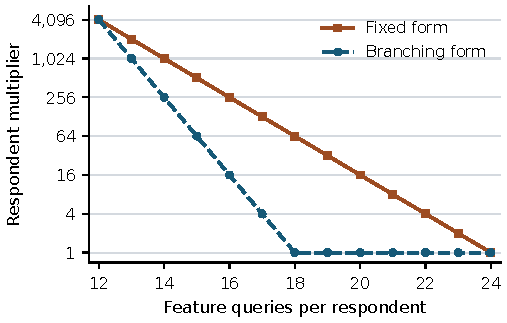
\includegraphics[width=.62\textwidth]{figures/query_cost.pdf}
\caption{Exact synthetic budget curve for the same contrast on 24 features ($k=6$). The fixed coefficient is 64 and the branching coefficient is one at 18 queries.}
\label{fig:cost}
\end{figure}



\section{Rounds of Adaptivity}\label{app:D}
\subsection{Rounds of Adaptivity}\label{app:roundshier}
\paragraph{Interviews with $r$ rounds.}
An $r$-round interview chooses coordinate batches
$B_1,\;B_2(x_{B_1}),\;\ldots,\;B_r(x_{B_1\cup\cdots\cup B_{r-1}})$.
Each batch is a function of the answers to earlier batches only, and
$\sum_s|B_s|\le b$ on every input. Let $\A_r(b)$ be the finite menu of
deterministic $r$-round interviews and $V_r(d,b)=V(d,\A_r(b))$; randomized
interviews are mixtures and are already represented by the design
probabilities in \eqref{eq:unbiasedprogram}. Fixed forms are $\A_1(b)$.
Sequentializing each batch shows that every $r$-round interview is a depth-$b$
tree, and a depth-$b$ tree is a $b$-round interview with one query per round.
Hence $\A_1(b)\subseteq\A_2(b)\subseteq\cdots\subseteq\A_b(b)=\A_{\rm branch}(b)$
and $V_1\ge V_2\ge\cdots\ge V_b=V_{\rm branch}$. All menus identify the same
contrasts, $\deg(d)\le b$, because the two extreme menus do
(Appendix~\ref{app:id}). Theorems~\ref{thm:finite} and~\ref{thm:asym} apply to
each finite menu $\A_r(b)$, so the lower bounds below hold against biased,
sequential and label-dependent procedures.

\begin{theorem}[Rounds of adaptivity, full statement of Theorem~\ref{thm:rounds}]\label{thm:roundsfull}
\textup{(a)} For $1\le r\le b\le m$ and every nonzero contrast of degree at most $b$ on $\{-1,1\}^m$,
\[
 V_{\rm branch}(d,b)\le V_r(d,b)\le
 \min\Big\{2^{b-r},\binom{m-r}{b-r}\Big\}\,V_{\rm branch}(d,b).
\]
\textup{(b)} For integers $r,\kappa\ge1$ put $D=2^\kappa$ and $b=r\kappa+1$.
The pointer-chasing contrast $N_{r,\kappa}$ defined below satisfies
\[
 V_{r+1}(N_{r,\kappa},b)=V_{\rm branch}(N_{r,\kappa},b)=1,\qquad
 \frac{D}{b}\le V_r(N_{r,\kappa},b)\le D.
\]
\end{theorem}

\begin{corollary}[Two rounds can be exponentially worse than branching]\label{cor:tworounds}
For every $b\ge3$,
\[
 \sup_{m,d}\frac{V_2(d,b)}{V_{\rm branch}(d,b)}\ \ge\ \frac{2^{\lfloor(b-1)/2\rfloor}}{b},
 \qquad
 \sup_{m,d}\frac{V_r(d,b)}{V_{r+1}(d,b)}\ \ge\ \frac{2^{\lfloor(b-1)/r\rfloor}}{b}
 \quad(1\le r<b).
\]
\end{corollary}
\begin{proof}
Take $\kappa=\lfloor(b-1)/r\rfloor\ge1$ and $N_{r,\kappa}$, which uses
$r\kappa+1\le b$ queries along every path. Branching and $(r+1)$-round
interviews still compute it exactly under the larger cap $b$, while the hit
bound in the proof of part (b) uses only the total number $b$ of queries.
For the first display use $r=2$ and $V_{\rm branch}\le V_3$.
\end{proof}

The constant separation $V_2\ge4/3$ of Corollary~\ref{cor:roundseparation}
is therefore not the end of the hierarchy. Part (b) and the corollary place
the exponent for $2\le r<b$ between $\lfloor(b-1)/r\rfloor-\log_2b$ and $b-r$;
the binary pointer tree (Theorem~\ref{thm:binarytree}) raises the lower end to
$b-1-r\log_2(1+2b/r)$, its products do so in polynomial dimension, and
Appendix~\ref{app:pointerexact} computes the constants of the tree at small caps.

\paragraph{Proof of part (a).}
The left inequality is menu inclusion. For the right inequality pad a
depth-$b$ tree $\tau$ as in Appendix~\ref{app:universal}, so that every path
has $b$ distinct coordinates. In rounds $1,\ldots,r-1$ ask one question per
round and follow $\tau$ exactly. This reaches a node $v$ of depth $r-1$,
whose padded subtree has depth $b-r+1$. Its path sets all contain the subtree
root and are determined by the first $b-r$ answers below $v$; hence their
number $L_v$ is at most $2^{b-r}$, and also at most $\binom{m-r}{b-r}$
because the remaining $b-r$ coordinates are chosen from the $m-r$
coordinates not on the followed prefix or at $v$. In round $r$ choose one of
these $L_v$ sets uniformly, independently of the person, and attempt to
complete the path. On completion return $L_v$ times the tree score and
otherwise zero. Conditionally on $x$ the mean equals the tree score and the
second moment is $L_v$ times its square. The mixture and merging argument of
Appendix~\ref{app:universal} applies verbatim to randomized branching
designs, so every feasible branching design is simulated with second
moment inflated by at most $\max_vL_v$.

\paragraph{The pointer-chasing contrast.}
Levels $\ell=1,\ldots,r$ consist of registers. Level $\ell$ has $D^{\ell-1}$
registers $R_\ell(i_1,\ldots,i_{\ell-1})$, indexed by
$(i_1,\ldots,i_{\ell-1})\in[D]^{\ell-1}$, and each register stores $\kappa$
binary coordinates encoding an element of $[D]$. There are $D^r$ data
coordinates $Z_{i_1\cdots i_r}$. The pointer path is $j_1=R_1$ and
$j_\ell=R_\ell(j_1,\ldots,j_{\ell-1})$, and
\[
 N_{r,\kappa}(x)=Z_{j_1\cdots j_r}
 =\sum_{i\in[D]^r}Z_i\prod_{\ell=1}^r\mathbf 1\{R_\ell(i_{<\ell})=i_\ell\}.
\]
Each register indicator has degree $\kappa$, so $\deg N_{r,\kappa}=r\kappa+1=b$.
Reading the $\kappa$ coordinates of the level-$\ell$ register on the pointer
path in round $\ell$, and the selected data coordinate in round $r+1$,
computes the contrast with $b$ queries in $r+1$ rounds. With Jensen's
inequality this gives $V_{r+1}=V_{\rm branch}=1$. For the upper bound
$V_r\le D$, read the pointer registers of levels $1,\ldots,r-1$ in the first
$r-1$ rounds. In round $r$, read the level-$r$ register together with one
data coordinate $Z_{j_1\cdots j_{r-1}J}$, where $J$ is uniform on $[D]$ and
drawn in advance. The score $DZ_{j_1\cdots j_{r-1}J}\mathbf 1\{J=j_r\}$ is
unbiased with second moment $D$ at every profile.

\paragraph{The lower bound $V_r(N_{r,\kappa},b)\ge D/b$.}
Let $\U$ be the uniform law and write $c^\star=(j_1,\ldots,j_r)$ for the
selected data cell. Since $\E_\U[N^2]=1$, the dual formula~\eqref{eq:vdual}
with witness $h=N$ gives $V_r\ge1/\max_{\iota\in\A_r(b)}E_\iota$, where
$E_\iota=\E_\U[\E_\U[N\mid\ell_\iota(X)]^2]$. Fix a deterministic $r$-round
interview $\iota$.

\emph{Step 1: a generous transcript.}
Let $\iota^+$ ask the same questions as $\iota$, but at the end of every
round additionally reveal the full content of every register touched in that
round. The transcript of $\iota$ is a function of that of $\iota^+$, and
conditional expectation onto a larger $\sigma$-field cannot decrease the
second moment, so $E_\iota\le E_{\iota^+}$.

\emph{Step 2: only the selected data coordinate carries signal.}
Let ${\rm Obs}$ be the set of data coordinates queried by $\iota^+$. For a
data cell $c$, on the transcript event $\{c\notin{\rm Obs}\}$ the transcript
and the pointer path are functions of the coordinates other than $Z_c$,
because the interview never reads $Z_c$. Since $Z_c$ is an independent
uniform sign, $\E[Z_c\mathbf 1\{c^\star=c\}\mid\ell_{\iota^+}]$ vanishes there.
Hence
\[
 \E[N\mid\ell_{\iota^+}]=\sum_{c\in{\rm Obs}}Z_c\,\PP(c^\star=c\mid\ell_{\iota^+}),
\]
so $|\E[N\mid\ell_{\iota^+}]|\le\PP(c^\star\in{\rm Obs}\mid\ell_{\iota^+})\le1$ and
\[
 E_{\iota^+}\le\E\big[\PP(c^\star\in{\rm Obs}\mid\ell_{\iota^+})\big]
 =\PP(c^\star\in{\rm Obs}).
\]

\emph{Step 3: observing $c^\star$ in $r$ rounds requires a lucky guess.}
Let $\G_t$ be the $\sigma$-field of the $\iota^+$ transcript before round $t$,
and let $K_t$ be the largest $k$ such that the pointer registers
$R_1,R_2(j_1),\ldots,R_k(j_{<k})$ are all revealed before round $t$; thus
$K_1=0$ and $K_t$ is nondecreasing. A query of round $t$ is \emph{deep} if it
touches a register of level at least $K_t+2$ or a data coordinate while
$K_t\le r-1$; it is a \emph{hit} if, in addition, the touched register or
data coordinate lies on the pointer path. Every deep location is indexed by a
tuple whose $(K_t+1)$st entry is $\G_t$-measurable, and lies on the pointer
path only if this entry equals $j_{K_t+1}$. The latter is the content of the
register $R_{K_t+1}(j_{\le K_t})$, which is unrevealed before round $t$.
For an adaptive sequence of queries to independent uniform coordinates, the
unrevealed coordinates remain independent and uniform given the
transcript. Hence $j_{K_t+1}$ is uniform on $[D]$ given $\G_t$, and every deep
query is a hit with conditional probability at most $1/D$.

If no hit occurs in rounds $1,\ldots,t$, then $K_{t+1}\le K_t+1$. Indeed,
$K_{t+1}\ge K_t+2$ requires the pointer register of level $K_t+2$ to be
revealed by the end of round $t$, say in round $t'\le t$. Since
$K_{t'}\le K_t$, that query was deep in round $t'$ and lay on the pointer path,
so it was a hit. By induction, without hits $K_t\le t-1\le r-1$ for every
$t\le r$. Then every query of a data coordinate in rounds $1,\ldots,r$ is deep,
and $c^\star$ can be queried only by a hit. Since the total number of queries
is at most $b$,
\[
 \PP(c^\star\in{\rm Obs})\le\PP(\text{some hit})
 \le\E\Big[\sum_{t=1}^r\sum_{\text{deep queries of round }t}\PP(\text{hit}\mid\G_t)\Big]
 \le\frac bD .
\]
Combining the three steps gives $E_\iota\le b/D$ for every $\iota\in\A_r(b)$,
and therefore $V_r\ge D/b$. \hfill$\square$

\paragraph{A binary pointer tree: few rounds lose almost the whole exponent.}
The pointer-chasing family separates consecutive numbers of rounds, but its
lower bound $2^{\lfloor(b-1)/r\rfloor}/b$ leaves the exponent for a fixed
small number of rounds far below the upper bound $b-r$ of part~(a). The
following contrast closes most of this gap. Let $L\ge1$ and $\beta=L+1$.
Arrange $2^L-1$ \emph{pointer coordinates} as the internal nodes $u$ of a
complete binary tree with levels $0,\ldots,L-1$ and attach $2^L$ \emph{data
coordinates} $Z_v$ to its leaves $v$, so that a block has $2^{\beta}-1$
coordinates. Encode the pointer coordinate of node $u$ as a bit
$x_u\in\{0,1\}$ that selects one of the two children of $u$. The
\emph{pointer path} starts at the root and descends through the selected
children; let $c^\star(x)$ be the leaf it reaches, and
\[
 B_L(x)=Z_{c^\star(x)}=\sum_{v}Z_v\prod_{u\in{\rm path}(v)}\mathbf 1\{x_u\to v\},
\]
where ${\rm path}(v)$ is the set of the $L$ internal nodes above $v$ and
$\{x_u\to v\}$ is the event that the bit of $u$ selects the child on the way
to $v$. Each indicator has degree one, so $\deg B_L=L+1=\beta$, and following
the path with one question per round computes $B_L$ with $\beta$ queries. The
function is the tree evaluation problem of \citet{cook2012}, and round
hierarchies for the query cost of oracle evaluation under bounded adaptivity
are known \citep{canonne2018,li2026regex}. Here the total number of queries is capped, exact
evaluation in fewer than $\beta$ rounds is impossible for every strategy, and
we quantify the variance that the missing rounds cost. To reach polynomial
dimension we also take products: for $k\ge1$ let
\[
 B_L^{\otimes k}(x^{(1)},\ldots,x^{(k)})=\prod_{i=1}^kB_L(x^{(i)})
\]
on $k$ disjoint blocks, a contrast of degree $k\beta$ on $k(2^\beta-1)$
coordinates.

\begin{theorem}[Binary pointer trees and their products]\label{thm:binarytree}
Let $L\ge1$, $\beta=L+1$, $k\ge1$ and $b\ge k\beta$, and let
$d=B_L^{\otimes k}$ on $m=k(2^\beta-1)$ coordinates.
\textup{(a)} $V_{\rm branch}(d,b)=1$ and $V_r(d,b)\le2^{b-r}$ for
$1\le r\le b$.
\textup{(b)} For every $1\le r\le b$,
\[
 V_r(d,b)\ \ge\ \frac{2^{k(\beta-1)}}{\big(1+\tfrac{2b}{rk}\big)^{rk}} .
\]
In particular the single tree $B_{b-1}$ on $m=2^b-1$ coordinates ($k=1$,
$\beta=b$) satisfies $V_r(B_{b-1},b)\ge2^{b-1}/(1+2b/r)^r$, and
$V_1(B_{b-1},b)\ge2^{b-1}/b$.
\end{theorem}

\begin{corollary}[Few rounds lose almost the whole exponent]\label{cor:fewrounds}
\textup{(i)} For every $b\ge2$ and $1\le r\le b$,
\[
 \frac{2^{b-1}}{(1+2b/r)^{r}}\ \le\ \sup_{m,d}\frac{V_r(d,b)}{V_{\rm branch}(d,b)}\ \le\ 2^{b-r},
 \qquad\text{in particular}\quad
 \frac{2^{b-1}}{(b+1)^2}\ \le\ \sup_{m,d}\frac{V_2(d,b)}{V_{\rm branch}(d,b)}\ \le\ 2^{b-2}.
\]
Hence for every fixed $r$ the exponent of the $r$-round gap is $b-O(r\log b)$.
\textup{(ii)} An $r$-round protocol that is within a factor $b^{c}$ of full
branching on every contrast of degree at most $b$ needs
$r\log_2(1+2b/r)\ge b-1-c\log_2b$, and therefore $r\ge0.37\,b-(1+c\log_2b)$
rounds: a number of rounds linear in the cap. The witnessing contrast is the
single tree $B_{b-1}$ on $2^b-1$ coordinates.
\textup{(iii)} Polynomial dimension. For every $b\ge4$ and $r\ge1$, with
$\beta=\lfloor\log_2b\rfloor$ and $k=\lfloor b/\beta\rfloor$, the contrast
$B_{\beta-1}^{\otimes k}$ has degree at most $b$, lives on $m\le b^2$
coordinates, and satisfies $V_{\rm branch}=1$ and
\[
 \log_2V_r\ \ge\ \Big(\frac b\beta-1\Big)(\beta-1)-\frac{rb}{\beta}\log_2\Big(1+\frac{4\beta}{r}\Big)
 \ =\ b-O\Big(\frac{r\,b\log\log b}{\log b}\Big)\quad(b\to\infty,\ r\text{ fixed}).
\]
\end{corollary}
\begin{proof}
(i) The upper bound is Theorem~\ref{thm:roundsfull}(a) and the lower bound is
Theorem~\ref{thm:binarytree}(b) with $k=1$. (ii) Combine $V_r\le b^c$ with
(i) and take logarithms. The function $f(r)=r\log_2(1+2b/r)$ is increasing
and concave, and $f(\alpha^\star b)=b$ for the solution
$\alpha^\star\approx0.376$ of $\alpha\log_2(1+2/\alpha)=1$, where
$f'(\alpha^\star b)=\log_2(1+2/\alpha^\star)-2/((\alpha^\star+2)\ln2)>1.44$. By
concavity $f(r)\le b-1.44(\alpha^\star b-r)$ for $r\le\alpha^\star b$, so
$f(r)\ge b-1-c\log_2b$ forces
$r\ge\alpha^\star b-(1+c\log_2b)/1.44$. (iii) Here $2^\beta\le b$, so
$m=k(2^\beta-1)<kb\le b^2$, and $k\beta\le b<(k+1)\beta\le2k\beta$ gives
$b/k<2\beta$. Theorem~\ref{thm:binarytree}(b) and $k\ge b/\beta-1$,
$k\le b/\beta$ give the display; with $\beta=\lfloor\log_2b\rfloor$ the
subtracted terms are $O(b/\log b)$ and $O(rb\log\log b/\log b)$.
\end{proof}

For two rounds the bound of (i) exceeds one once $2^{b-1}>(b+1)^2$, that is
for $b\ge8$; for smaller caps Appendix~\ref{app:pointerexact} computes the
round constants of $B_{b-1}$ numerically (two rounds lose at least $1.80$ at
$b=3$ and $3.32$ at $b=4$). The single tree uses a number of coordinates
exponential in $b$, like the address contrast; part (iii) removes this at the
price of the lower-order term in the exponent, exactly as products of
address blocks do for fixed forms (Proposition~\ref{prop:productaddress}).
The product is, however, evaluated exactly in $\beta=\lfloor\log_2b\rfloor$
rounds within the cap: reading level $j$ of every block in round $j$ uses
$k\beta\le b$ questions. Part (iii) therefore gives a lower bound only for
$r=o(\log b/\log\log b)$, and the linear number of rounds in (ii) is proved
only for the single tree, with exponentially many coordinates; whether more
than logarithmically many rounds can be necessary on a number of coordinates
polynomial in $b$ is open.
Whether the factor $(1+2b/r)^r$ can be removed, so that the $r$-round gap is
$2^{b-r}$ up to constants, is open.

\paragraph{Proof of Theorem~\ref{thm:binarytree}.}
(a) Following the pointer path of every block returns $d$ itself with
$k\beta\le b$ queries, so $V_{\rm branch}\le1$; every unbiased design has
$\sum_\iota g_\iota(x)=d(x)=\pm1$, and Cauchy--Schwarz gives
$\sum_\iota g_\iota(x)^2/q_\iota\ge1$ at every $x$, so $V_{\rm branch}\ge1$.
The remaining inequality is Theorem~\ref{thm:roundsfull}(a).

(b) Let $\U$ be the uniform law on all coordinates. Under $\U$ the blocks
are independent, $\E_\U[d^2]=1$, and the pointer path of each block is a
uniformly distributed root-to-leaf path. By the dual
formula~\eqref{eq:vdual} with witness $h=d$,
$V_r(d,b)\ge1/\max_{\iota\in\A_r(b)}E_\iota$ with
$E_\iota=\E_\U[\E_\U[d\mid\ell_\iota(X)]^2]$. Fix a deterministic $r$-round
interview $\iota$. Let $S_t$ be the set of coordinates it reads in round $t$;
$S_t$ is a function of the transcript $T_{t-1}$ of rounds $1,\ldots,t-1$, and
we may assume that no coordinate is read twice. For block $i$ write
$a_{t,i}$ and $\lambda_{t,i}$ for the numbers of its pointer and data
coordinates in $S_t$ and $n_{t,i}=a_{t,i}+\lambda_{t,i}$, so that
$\sum_{t,i}n_{t,i}\le b$; let $I_{t,i}$ be the set of pointer coordinates of
block $i$ read in rounds $1,\ldots,t$, ${\rm Obs}_{t,i}$ the set of its leaves
whose data coordinate is read in rounds $1,\ldots,t$, and $c^\star_i$ the leaf
selected in block $i$.

\emph{Step 1: only selected leaves carry signal.}
The event $\{T_r=\tau\}$ fixes the values of the coordinates read under
$\tau$ and nothing else, so conditionally on the transcript the unread
coordinates remain independent and uniform and the blocks remain
independent. Hence
$\E_\U[d\mid\ell_\iota]=\prod_i\E_\U[B_L(X^{(i)})\mid\ell_\iota]$. Within a
block, the data coordinate of an unread leaf $v$ is independent of the
transcript and of the pointer path, so
$\E_\U[Z_v\mathbf 1\{c^\star_i=v\}\mid\ell_\iota]=0$, and
\[
 \big|\E_\U[B_L(X^{(i)})\mid\ell_\iota]\big|
 =\Big|\sum_{v\in{\rm Obs}_{r,i}}Z_v\,\PP(c_i^\star=v\mid T_r)\Big|
 \le\pi_{r,i},\qquad \pi_{t,i}:=\PP(c_i^\star\in{\rm Obs}_{t,i}\mid T_t).
\]
Since $0\le\pi_{r,i}\le1$,
\begin{equation}
 E_\iota\le\E\Big[\prod_{i=1}^k\pi_{r,i}^2\Big]\le\E\Big[\prod_{i=1}^k\pi_{r,i}\Big].\label{eq:allhit}
\end{equation}

\emph{Step 2: the conditional law of a selected leaf.}
For a leaf $v$ of block $i$ let $R_t(v)=|{\rm path}(v)\cap I_{t,i}|$ be the
number of pointer coordinates on its path read by the end of round $t$, and
let $C_t(v)$ be the event that every one of them selects the child towards
$v$. Since $c_i^\star=v$ exactly when all $L$ pointer coordinates on
${\rm path}(v)$ select the child towards $v$, and the unread ones are
uniform given $T_t$,
\begin{equation}
 \PP(c_i^\star=v\mid T_t)=\mathbf 1\{C_t(v)\}\,2^{R_t(v)-L}.\label{eq:leaflaw}
\end{equation}

\emph{Step 3: a potential for one block.}
Put $M_{t,i}=\max_v\mathbf 1\{C_t(v)\}2^{R_t(v)}$ over the leaves of block
$i$, so that $M_{0,i}=1$ and, by \eqref{eq:leaflaw},
$\max_v\PP(c_i^\star=v\mid T_t)=M_{t,i}2^{-L}$, and put
\[
 Q_{t,i}=M_{t,i}+2^L\pi_{t,i},\qquad Q_{0,i}=1 .
\]
We claim
\begin{equation}
 \E[Q_{t,i}\mid T_{t-1}]\le(1+2a_{t,i}+\lambda_{t,i})\,Q_{t-1,i}\le(1+2n_{t,i})\,Q_{t-1,i}.\label{eq:potential}
\end{equation}
\emph{The most likely leaf.} We show
$\E[M_{t,i}\mid T_{t-1}]\le(1+2a_{t,i})M_{t-1,i}$. Condition on $T_{t-1}$,
which fixes $S_t$, drop the block index, and let $v^\star$ attain $M_t$. If no
coordinate of $S_t$ lies on ${\rm path}(v^\star)$, then
$R_t(v^\star)=R_{t-1}(v^\star)$ and $C_t(v^\star)=C_{t-1}(v^\star)$, so
$M_t\le M_{t-1}$. Otherwise let $u$ be the deepest node of
${\rm path}(v^\star)\cap S_t$, write ${\rm path}(u)$ for the nodes above $u$
together with $u$ itself, and define
\[
 G(u)=\mathbf 1\{\text{every node of }({\rm path}(u)\setminus\{u\})\cap I_t\text{ selects towards }u\}\,2^{|{\rm path}(u)\cap I_t|},
\]
\[
 F(u)=\max_{w\text{ below }u}\mathbf 1\{\text{every node of }({\rm path}(w)\setminus{\rm path}(u))\cap I_{t-1}\text{ selects towards }w\}\,2^{|({\rm path}(w)\setminus{\rm path}(u))\cap I_{t-1}|}.
\]
No node of ${\rm path}(v^\star)$ strictly below $u$ is read in round $t$, so
every read node there belongs to $I_{t-1}$ and
$\mathbf 1\{C_t(v^\star)\}2^{R_t(v^\star)}\le G(u)F(u)$: the factor $G(u)$
accounts for the nodes of ${\rm path}(u)$ other than $u$ and for the count
including $u$, the bound $\mathbf 1\{x_u\to v^\star\}\le1$ drops $u$'s own
selection, and $F(u)$ dominates the contribution of the nodes below $u$
because $w=v^\star$ is admissible in its maximum. Consequently
$M_t\le M_{t-1}+\sum_{u\in S_t\cap U}G(u)F(u)$, the sum being over the
pointer coordinates of the block in $S_t$. The quantity $F(u)$ is
$T_{t-1}$-measurable. Given $T_{t-1}$, the $|{\rm path}(u)\cap S_t|-1$ newly
read nodes strictly above $u$ select towards $u$ independently with
probability $1/2$ each, so
\[
 \E[G(u)\mid T_{t-1}]
 =\mathbf 1\{\text{every node of }{\rm path}(u)\cap I_{t-1}\text{ selects towards }u\}\,
   2^{|{\rm path}(u)\cap I_{t-1}|}\cdot2 .
\]
Multiplying by $F(u)$ reassembles, for the leaf $w$ below $u$ attaining
$F(u)$, exactly $2\cdot\mathbf 1\{C_{t-1}(w)\}2^{R_{t-1}(w)}\le2M_{t-1}$,
because $u\notin I_{t-1}$. Summing over the $a_t$ pointer coordinates of the
block in $S_t$ proves the claim.

\emph{The leaves already read.} The sets ${\rm Obs}_{t-1,i}$ and $S_t$ are
$T_{t-1}$-measurable and disjoint, so
$\pi_{t,i}=\PP(c_i^\star\in{\rm Obs}_{t-1,i}\mid T_t)+\PP(c_i^\star\in S_t\mid T_t)$
(we write $c_i^\star\in S_t$ when the data coordinate of that leaf is read in round $t$),
and by the tower property and \eqref{eq:leaflaw},
\[
 \E[\pi_{t,i}\mid T_{t-1}]
 =\pi_{t-1,i}+\PP(c_i^\star\in S_t\mid T_{t-1})
 \le\pi_{t-1,i}+\lambda_{t,i}\,M_{t-1,i}\,2^{-L}.
\]
Adding $2^L$ times this inequality to the bound for $M_{t,i}$ gives
$\E[Q_{t,i}\mid T_{t-1}]\le(1+2a_{t,i}+\lambda_{t,i})M_{t-1,i}+2^L\pi_{t-1,i}$,
which is~\eqref{eq:potential}.

\emph{Step 4: blocks multiply.}
Given $T_{t-1}$ the batch $S_t$ is fixed, the answers of round $t$ in
different blocks are independent, and $Q_{t,i}$ is a function of $T_{t-1}$
and of the round-$t$ answers in block $i$. Hence
$\E[\prod_iQ_{t,i}\mid T_{t-1}]=\prod_i\E[Q_{t,i}\mid T_{t-1}]\le\prod_i(1+2n_{t,i})\prod_iQ_{t-1,i}$.
Let $\Psi_t=\prod_iQ_{t,i}\prod_{s\le t}\prod_i(1+2n_{s,i})^{-1}$. As the
$n_{t,i}$ are $T_{t-1}$-measurable, $\E[\Psi_t\mid T_{t-1}]\le\Psi_{t-1}$ and
$\E[\Psi_r]\le\Psi_0=1$.

\emph{Step 5: combination.}
The pathwise constraint $\sum_{t\le r}\sum_in_{t,i}\le b$ and the inequality
between arithmetic and geometric means over the $rk$ pairs $(t,i)$ give
$\prod_{t\le r}\prod_i(1+2n_{t,i})\le(1+2b/(rk))^{rk}$. Since
$2^L\pi_{r,i}\le Q_{r,i}$,
\[
 \E\Big[\prod_{i=1}^k\pi_{r,i}\Big]\le2^{-Lk}\,\E\Big[\prod_iQ_{r,i}\Big]
 =2^{-Lk}\,\E\Big[\Psi_r\prod_{t\le r}\prod_i(1+2n_{t,i})\Big]
 \le2^{-k(\beta-1)}\Big(1+\frac{2b}{rk}\Big)^{rk}.
\]
With \eqref{eq:allhit} and the dual formula this proves the first statement
of (b). For $r=1$ and $k=1$, \eqref{eq:leaflaw} at $t=0$ gives directly
$\PP(c^\star\in{\rm Obs})\le\lambda_12^{-L}\le b2^{-L}$, which is the last
statement. \hfill$\square$

The argument is a potential-function version of the lucky-hit bound: a
round can raise the conditional probability of the most likely leaf only by
a factor linear in the number of pointer coordinates it reads, whereas
following the path raises it by a factor two per question; the potential
$Q$ adds the probability that a leaf already read is the selected one, which
makes the bound multiplicative across blocks even though an interview may
split its questions among blocks adaptively. As a numerical check, the
released code verifies \eqref{eq:potential} exhaustively on the tree with
$L=2$ (all 4,752 pairs of a state and a nonempty batch; the largest ratio of
the two sides is exactly one) and on random states and batches for $L=3$
and $L=4$ (largest ratio one and $0.83$).


\paragraph{Interpretation.}
Each round can advance the known part of the pointer path by at most one
level unless a question lands on an unknown pointer target, which happens
with probability at most $1/D$ per question. Additional questions within a
round therefore do not substitute for a round. Practical counterparts of
rounds are questionnaire pages, clinic visits and batches of laboratory
orders. The address contrast of Theorem~\ref{thm:universal} is the case
$r=1$, where two rounds already attain the branching coefficient. The
pointer-chasing family shows that this is not a general property of
two-stage designs.

\subsection{Two Rounds Already Attain the Universal Extremum}\label{app:rounds}
An $R$-round interview uses at most $R$ batches, choosing each batch of coordinates using only the preceding batches' answers, with at most $b$ coordinates in total. Let $V_R$ use all such interviews. One round is the fixed-form menu and $b$ rounds suffice for full branching. For any $R\ge2$,
\[
 1\le V_{\rm fixed}/V_R\le K_{m,b},\qquad
 \sup_{m,d\ne0}\frac{V_{\rm fixed}(d,b)}{V_R(d,b)}=2^{b-1},
\]
where the supremum is over identifiable binary contrasts. The upper bound follows from menu inclusion. The address construction attains equality using two batches: all address bits, then the addressed data bit. Thus the universal extremum measures the value of permitting a second batch; it does not require $b$ sequential rounds.

The block construction also needs at most two rounds throughout its identifiable budget curve. At $b=2k+R$, $0\le R\le k$, use the paper's three-query strategy on $R$ blocks and two-query strategy on the others. Ask the first two queries in every block together; then ask the selected third coordinate in the $R$ adaptive blocks. At $b\ge3k$ this already evaluates the contrast exactly. The address and block examples do not separate two rounds from unrestricted branching. Corollary~\ref{cor:roundseparation} supplies a constant separation with a four-feature contrast, and the pointer constructions of Appendix~\ref{app:roundshier} supply the exponential hierarchy.

\subsection{Labels and Across-Person Adaptation}
Let $R_{\rm pre}$ require selecting the interview independently of the current label, and let $R_{\rm label}$ allow observing that label first, while both permit adaptation across people. For an identifiable contrast, Theorem~\ref{thm:asym} and the iid upper construction imply
\[
 \lim_{n\to\infty}nR_{\rm pre}(d,n)
 =\lim_{n\to\infty}nR_{\rm label}(d,n)=V(d,\A).
\]
Thus neither access to earlier people nor early access to the current label reduces the first-order worst-case coefficient relative to an optimal iid design.

There is also an exact statement for the \emph{finite program}. If one extends $\Phi_n$ to separate form laws and score tables for $y=-1,+1$, its objective is the maximum over these labels of their individual worst-profile quadratic objectives. Multiplying the negative-label tables by $-1$ turns both subproblems into the definition of $\Phi_n(d,\A)$. Each has value at least $\Phi_n$, and using the same form law and sign-adjusted tables attains it. Early labels therefore do not improve this program. This is not an equality claim for the exact finite-$n$ minimax risks, which the program bounds only within a constant.

\subsection{Round Constants of the Binary Pointer Tree at Small Caps}\label{app:pointerexact}
The two-round bound of Theorem~\ref{thm:rounds}(b) exceeds one only for $b\ge8$. For small caps we compute the round constants of $B_{b-1}$ directly. Under the uniform law $\U$ with a label independent of the profile, $M_r(\U)$, the optimal second moment over $r$-round designs, is a lower bound on $V_r$, because $V_r=\sup_PM_r(P)$ by Sion's theorem applied to \eqref{eq:unbiasedprogram}. For $b\le4$ the cube is small enough to evaluate the uniform-optimal design at every profile; its worst profile is an upper bound on $V_r$. The solver of Appendix~\ref{app:engine} computes $M_r(\U)$ with certified bounds that agree to $10^{-7}$ or better.
\input{v20_pointer_table}
At $b=3$ and $b=4$ the two bounds agree to the reported precision except for two rounds at $b=4$, where they differ by 0.3\%. Two rounds therefore lose almost the factor $2^{b-2}$ allowed by Theorem~\ref{thm:rounds}(a) already at these caps, and each missing round costs a factor close to two. The cap $b=5$ ($m=31$, 169,911 forms) was not completed.



\section{Population Constants and Their Computation}\label{app:E}
\subsection{The Value of Adaptivity at a Given Population}\label{app:population}
Fix a menu $\A$ and a law $P$ on $\X\times\{-1,1\}$. A \emph{design} is a
probability vector $(q_\iota)$ on $\A$ with tables $g_\iota(\ell,y)$ that
satisfy $\sum_\iota g_\iota(\ell_\iota(x),y)=t(x,y)=yd(x)$ for all $(x,y)$.
Its score is $H=g_\iota(\ell_\iota(X),Y)/q_\iota$ with $\iota\sim q$ drawn
independently of the record, which is unbiased for $t$ at every profile and
label; conversely every function $H$ of $(\iota,\ell_\iota(X),Y)$ with
$\E[H\mid X,Y]=t$ arises in this way. $W_\A(P)$ is the infimum of
$\Var_{P,q}(H)$ over designs, $M_\A(P)=W_\A(P)+\Delta(P)^2$ the infimum of
the second moment, and $\sigma_P^2=\Var_P(t)$. At a full-support law,
$W_\A(P)$ is also the local asymptotic minimax risk over arbitrary estimators
(Proposition~\ref{prop:local}), so ratios of $W$ are ratios of the numbers of
records that two menus need. For a deterministic depth-$b$ tree $\tau$ that
computes $d$, $S_\tau(x)$ is its padded path set and $\mathcal S_\tau$ the
collection of these sets (Appendix~\ref{app:universal}).

\begin{theorem}[Records needed at a population, full statement of Theorems~\ref{thm:universal}(ii), \ref{thm:rounds}(a) and~\ref{thm:bracket}]\label{thm:bracketfull}
Let $d$ be a nonzero contrast of degree at most $b$ on $\{-1,1\}^m$ and $P$ any
law on $\X\times\{-1,1\}$.

\textup{(a) Uniform gap.} For $1\le r\le b$,
\[
 W_{\rm branch}(P)\ \le\ W_r(P)\ \le\ \min\Big\{2^{b-r},\binom{m-r}{b-r}\Big\}\,W_{\rm branch}(P),
\]
and in particular $W_{\rm fixed}(P)\le K_{m,b}W_{\rm branch}(P)$.

\textup{(b) Witness bound.} For every menu $\A$, every constant $c$ and
every function $h$ on $\X\times\{-1,1\}$ with $\E_P[(t-c)h]\ne0$,
\[
 W_\A(P)+(\Delta(P)-c)^2\ \ge\ \frac{\E_P[(t-c)h]^2}{\max_{\iota\in\A}\E_P\big[\E_P[h\mid\ell_\iota(X),Y]^2\big]}.
\]
With $c=0$ this bounds the second moment $M_\A(P)$, and with $c=\Delta(P)$ it
bounds the variance $W_\A(P)$.

\textup{(c) Bracket.} If a depth-$b$ tree $\tau$ computes $d$ and
$\sigma_P^2>0$, then $W_{\rm branch}(P)=\sigma_P^2$ and
\[
 \frac1{\rho_P^2}\ \le\ \frac{W_{\rm fixed}(P)}{W_{\rm branch}(P)}\ \le\ N_P(\tau)\ \le\ |\mathcal S_\tau|\ \le\ K_{m,b},
\]
where
\[
 \rho_P^2=\max_{|T|=b}\frac{\Var_P\big(\E_P[t\mid X_T,Y]\big)}{\Var_P(t)},
 \qquad
 N_P(\tau)=\Big(\sum_{S\in\mathcal S_\tau}v_S^{1/2}\Big)^2,
 \quad v_S=\frac{\E_P\big[(t-\Delta(P))^2\mathbf 1\{S_\tau(X)=S\}\big]}{\sigma_P^2}.
\]
More generally $W_{\rm fixed}(P)\le\big(\sum_S\E_P[(t-c)^2\mathbf 1\{S_\tau(X)=S\}]^{1/2}\big)^2-(\Delta(P)-c)^2$
for every constant $c$.

\textup{(d)} For the address contrast with $\kappa=b-1$ under the uniform law
with independent uniform labels, $1/\rho_P^2=N_P(\tau)=K_{m,b}=D$, so all
inequalities in \textup{(c)} are equalities.
\end{theorem}

The quantity $\rho_P^2$ is the largest fraction of the variance of the target
that a single form explains, a population $R^2$. The weights $v_S$ sum to
one, and $N_P(\tau)=\exp H_{1/2}(v)$ is the exponential of their R\'enyi
entropy of order $1/2$: an effective number of question sets that the tree
uses at $P$. Adaptivity can be valuable only when the tree's questions diverge
over many well-populated paths, and it is valuable when in addition no fixed
set of $b$ questions explains most of the variance of the target; correlated
features and shared coordinates raise $\rho_P^2$.

\begin{proof}
\emph{(a)} The left inequality is menu inclusion. For the right one fix a
branching design: trees $\tau$ with probabilities $q_\tau>0$ and tables
$g_\tau(\ell,y)$ with $\sum_\tau g_\tau(\ell_\tau(x),y)=t(x,y)$, and write
$H_\tau(x,y)=g_\tau(\ell_\tau(x),y)/q_\tau$, so that
$\sum_\tau q_\tau H_\tau=t$ pointwise. Pad every tree as in
Appendix~\ref{app:universal}; padding refines the transcript, so $H_\tau$
is still a function of the padded leaf and the label. For a node $v$ of
$\tau$ at depth $r-1$ (the root if $r=1$), the padded subtree below $v$ has
depth $b-r+1$; let $\mathcal S_{\tau,v}$ be the collection of coordinate sets
of its root-to-leaf paths and $L_{\tau,v}=|\mathcal S_{\tau,v}|$. These sets
contain the coordinate asked at $v$ and are determined by the first $b-r$
answers below $v$, so $L_{\tau,v}\le\min\{2^{b-r},\binom{m-r}{b-r}\}=:K_r$.
Fix a constant $c$ and consider the following randomized $r$-round interview
with at most $b$ queries. Draw $\tau\sim q$ and, independently of the record,
one set $S_v$ uniformly from $\mathcal S_{\tau,v}$ for every node $v$ of
depth $r-1$. In rounds $1,\ldots,r-1$ ask one question per round and follow
$\tau$ to a node $v$; in round $r$ ask the coordinates of $S_v$. The path of
$x$ below $v$ can be followed to a leaf exactly when its coordinate set equals
$S_v$, which has conditional probability $1/L_{\tau,v}$ given $(x,y,\tau)$,
and this event is measurable from the transcript. Return
\[
 \widetilde H=c+L_{\tau,v}\big(H_\tau(x,y)-c\big)\ \text{on completion},\qquad \widetilde H=c\ \text{otherwise}.
\]
The pair $(\tau,(S_v)_v)$ indexes a deterministic $r$-round interview, so
$\widetilde H$ is a score of a design on $\A_r(b)$. Conditionally on $(x,y)$
and $\tau$, its mean is $H_\tau(x,y)$ and
$\E[(\widetilde H-c)^2\mid x,y,\tau]=L_{\tau,v}(H_\tau(x,y)-c)^2\le K_r(H_\tau(x,y)-c)^2$.
Hence $\E[\widetilde H\mid X,Y]=t$, and with $H=H_\tau$ for $\tau\sim q$,
\[
 \Var(\widetilde H)=\E[(\widetilde H-c)^2]-(\Delta(P)-c)^2
 \le K_r\,\E[(H-c)^2]-(\Delta(P)-c)^2 .
\]
Choose $c=\Delta(P)$: then $\E[(H-c)^2]=\Var(H)$ and
$\Var(\widetilde H)\le K_r\Var(H)$. The constant $c$ is part of the score, not
an estimate: the design is pointwise unbiased for every value of $c$, and
$W_r(P)$ is by definition an infimum over designs that may be tuned to $P$.
Taking the infimum over branching designs proves (a).

\emph{(b)} Let $(q,g)$ be a design on $\A$ with score $H$. The tables
$g_\iota-cq_\iota$ sum to $t-c$, and
$\E[(H-c)^2]=\sum_\iota\|g_\iota-cq_\iota\|_P^2/q_\iota\ge(\sum_\iota\|g_\iota-cq_\iota\|_P)^2$
by Cauchy--Schwarz in $q$. For every $h$,
\[
 \E_P[(t-c)h]=\sum_\iota\E_P\big[(g_\iota-cq_\iota)\,\E_P[h\mid\ell_\iota(X),Y]\big]
 \le\Big(\sum_\iota\|g_\iota-cq_\iota\|_P\Big)\max_\iota\big\|\E_P[h\mid\ell_\iota(X),Y]\big\|_P,
\]
because $g_\iota-cq_\iota$ is a function of $(\ell_\iota(X),Y)$. Square, use
$\E[(H-c)^2]=\Var(H)+(\Delta(P)-c)^2$ and take the infimum over designs.

\emph{(c)} Following $\tau$ returns $t$ itself, and every unbiased score has
$\Var(H)\ge\Var(\E[H\mid X,Y])=\sigma_P^2$, so $W_{\rm branch}(P)=\sigma_P^2$.
For the lower bound apply (b) to the fixed forms with $c=\Delta(P)$ and
$h=t-\Delta(P)$: the numerator is $\sigma_P^4$ and
$\E_P[\E_P[t-\Delta\mid X_T,Y]^2]=\Var_P(\E_P[t\mid X_T,Y])$ because
$\E_P[t\mid X_T,Y]$ has mean $\Delta(P)$. For the upper bound choose $q_S>0$
on $\mathcal S_\tau$, draw $S$ before the person answers and return
$c+(t(X,Y)-c)/q_S$ if the tree's path completes inside $S$ and $c$ otherwise.
Completion occurs exactly when $S=S_\tau(X)$
(Appendix~\ref{app:universal}), so the score is unbiased at every profile and
label, and $\E[(H-c)^2]=\sum_Sq_S^{-1}\E_P[(t-c)^2\mathbf 1\{S_\tau(X)=S\}]$.
Minimizing over the simplex gives
$q_S\propto\E_P[(t-c)^2\mathbf 1\{S_\tau=S\}]^{1/2}$ and the value
$(\sum_S\E_P[(t-c)^2\mathbf 1\{S_\tau=S\}]^{1/2})^2$; sets of zero weight are
handled by letting their probability tend to zero. Subtracting
$(\Delta(P)-c)^2$ gives the general statement, and $c=\Delta(P)$ gives
$N_P(\tau)\sigma_P^2$. Finally $(\sum_Sv_S^{1/2})^2\le|\mathcal S_\tau|\sum_Sv_S=|\mathcal S_\tau|$
by Cauchy--Schwarz, and $|\mathcal S_\tau|\le K_{m,b}$.

\emph{(d)} Here $\Delta=0$, $t^2=1$ and the $D$ path sets are equally likely,
so $N_P=D=K_{m,b}$. With independent labels,
$\E[t\mid X_T,Y]=Y\E[d\mid X_T]$, whose second moment is at most $2^{-\kappa}=1/D$
by~\eqref{eq:addressinformation}, so $1/\rho_P^2\ge D$.
\end{proof}

\paragraph{Relation to the uncentered bracket.}
Setting $c=0$ in (b) and (c) gives the second-moment bracket
$\E_P[t^2]/\Gamma_P\le M_{\rm fixed}(P)\le N^0_P(\tau)\E_P[t^2]$ with
$\Gamma_P=\max_T\E_P[\E_P[t\mid X_T,Y]^2]/\E_P[t^2]$ and $N_P^0$ computed
from the weights $\E_P[t^2\mathbf 1\{S_\tau=S\}]$. Subtracting $\Delta^2$
turns it into a bracket for $W_{\rm fixed}/W_{\rm branch}$ with lower end
$(\E_P[t^2]/\Gamma_P-\Delta^2)/\sigma_P^2$ and upper end
$(N_P^0\E_P[t^2]-\Delta^2)/\sigma_P^2$. The centered lower end is never
smaller: writing $s=\E_P[t^2]$ and $e=\Gamma_Ps$, the claim
$(s-\Delta^2)^2\ge(s^2/e-\Delta^2)(e-\Delta^2)$ reduces to $s^2/e+e\ge2s$. The
uncentered upper end is unbounded as $\Delta^2\to\E_P[t^2]$, that is for
accurate rules, whereas the centered one never exceeds $K_{m,b}$; for the
worked example of Section~\ref{sec:setup} with uniform profiles and a label
that agrees with $d$ with probability $0.9$, the centered upper end is $2$ and
the uncentered one is $(2-0.8^2)/0.36\approx3.78$. Centering is what makes part (a) hold at every
population: without it, path guessing inflates the second moment by $K_r$
and the variance by more.

\paragraph{Label-dependent designs.}
Labels are observed before the questions are asked, so a collector may let
the interview probabilities depend on the label, as in outcome-dependent
two-phase sampling. Write $\A^{\rm lab}$ for this larger class of designs on a
menu $\A$: probability vectors $q_{\cdot\mid y}$ for $y=\pm1$ with tables that
sum to $t(\cdot,y)$ for each label.

\begin{proposition}[Label-dependent designs]\label{prop:labeldesign}
\textup{(i)} $V(d,\A)$ is unchanged if interview probabilities may depend on
the current label (Theorem~\ref{thm:asym}).
\textup{(ii)} For every law $P$, $M_{\A}^{\rm lab}(P)=\sum_{y=\pm1}M_\A(P^{(y)})$,
where $P^{(y)}=P(\cdot,y)$ is the sub-probability law of the profiles with
label $y$ and $M_\A(P^{(y)})$ is the optimum of the program for the target
$yd$ under that mass; hence $W^{\rm lab}_\A(P)=\sum_yM_\A(P^{(y)})-\Delta(P)^2\le W_\A(P)$.
\textup{(iii)} Part \textup{(a)} of Theorem~\ref{thm:bracketfull} holds for
label-dependent designs: $W^{\rm lab}_r(P)\le K_rW^{\rm lab}_{\rm branch}(P)$,
and $W^{\rm lab}_{\rm branch}(P)=\sigma_P^2$ when a depth-$b$ tree computes
$d$.
\end{proposition}
\begin{proof}
(i) The converse of Theorem~\ref{thm:asym} allows the interview to depend on
the current label, and label-independent designs attain $V$. (ii) The second
moment of a label-dependent design is
$\sum_y\sum_\iota\E_P[g_{\iota,y}(\ell_\iota(X))^2\mathbf 1\{Y=y\}]/q_{\iota\mid y}$,
and neither the constraints nor the probability vectors couple the two
labels. (iii) The simulation in the proof of
Theorem~\ref{thm:bracketfull}(a) is carried out separately for each label
with the same constant $c=\Delta(P)$; the conditional bound
$\E[(\widetilde H-c)^2\mid x,y]\le K_r\E[(H-c)^2\mid x,y]$ holds for each
$(x,y)$. The last statement is the Jensen bound.
\end{proof}
Each $M_\A(P^{(y)})$ is computed by the solver of Appendix~\ref{app:engine}
with the same certificates. Appendix~\ref{app:screendetail} reports that
label-dependent form probabilities lower the records ratio of the screening
trees by at most \nLabelMax\%, and by at most \nStratMax\% when they are also
stratified by sex.

\paragraph{Accurate populations.}
The populations that attain the worst-case constants in Appendices~\ref{app:C} and~\ref{app:D} have labels independent of the profile, so that the rule under audit is no better than chance. The gaps do not depend on this.

\begin{proposition}[The gaps persist at every accuracy]\label{prop:labelnoise}
Let $d$ take values in $\{-1,1\}$, let $X\sim\mu$ for an arbitrary profile law $\mu$, and let $Y=d(X)\xi$, where $\xi\in\{-1,1\}$ is independent of $X$ with $\PP(\xi=1)=p\in(0,1)$. Then $t=\xi$, $\Delta(P)=2p-1$, $\sigma_P^2=1-\Delta^2$, and for every interview $\iota$, with $e_\iota=\E_\mu[d\mid\ell_\iota(X)]$,
\[
 \Var_P\big(\E_P[t\mid\ell_\iota(X),Y]\big)=\sigma_P^4\,\E_\mu\Big[\frac{e_\iota^2}{1-\Delta^2e_\iota^2}\Big]\ \le\ \sigma_P^2\,\E_\mu[e_\iota^2].
\]
Consequently, for every menu $\A$,
\[
 \frac{W_\A(P)}{\sigma_P^2}\ \ge\ \frac1{\max_{\iota\in\A}\|\E_\mu[d\mid\ell_\iota(X)]\|_\mu^2},
\]
which is the bound that the dual of Theorem~\ref{thm:char} gives for $V(d,\A)$ with the witness $h=d$ at $\mu$. In particular:
\textup{(i)} for the address contrast with $\kappa=b-1$ and uniform profiles, $W_{\rm fixed}(P)/W_{\rm branch}(P)=2^{b-1}$ for every $p\in(0,1)$, that is, at every accuracy $(1+\Delta)/2$ of the rule;
\textup{(ii)} for the pointer-tree contrasts of Theorem~\ref{thm:binarytree} with uniform profiles, $W_r(P)/W_{\rm branch}(P)\ge2^{k(\beta-1)}(1+2b/(rk))^{-rk}$ for every $p\in(0,1)$.
\end{proposition}
\begin{proof}
Since $d^2=1$, $t=Yd(X)=\xi$. Fix $\iota$ and a transcript, and write $e$ for $e_\iota$ at that transcript, so that $\PP(d=\pm1\mid\ell_\iota)=(1\pm e)/2$. For $y\in\{-1,1\}$, $\PP(Y=y\mid\ell_\iota)=\tfrac12(1+e)\PP(\xi=y)+\tfrac12(1-e)\PP(\xi=-y)=\tfrac12(1+y\Delta e)$, and by Bayes' rule $\PP(d=y\mid\ell_\iota,Y=y)=p(1+ye)/(1+y\Delta e)$. Hence
\[
 \E_P[t\mid\ell_\iota,Y=y]=\frac{p(1+ye)-(1-p)(1-ye)}{1+y\Delta e}=\frac{\Delta+ye}{1+y\Delta e},
 \qquad
 \E_P[t\mid\ell_\iota,Y=y]-\Delta=\frac{ye\,\sigma_P^2}{1+y\Delta e}.
\]
Averaging the square over $y$ with the weights $\tfrac12(1+y\Delta e)$ gives $\tfrac12e^2\sigma_P^4[(1+\Delta e)^{-1}+(1-\Delta e)^{-1}]=e^2\sigma_P^4/(1-\Delta^2e^2)$, and taking the expectation over the transcript proves the identity. The inequality uses $e^2\le1$, so that $1-\Delta^2e^2\ge\sigma_P^2$. The bound on $W_\A$ is Theorem~\ref{thm:bracketfull}(b) with $c=\Delta$ and $h=t-\Delta$, whose numerator is $\sigma_P^4$.
(i) Branching computes $d$, so $W_{\rm branch}(P)=\sigma_P^2$; the energy of every form is at most $2^{-\kappa}$ by~\eqref{eq:addressinformation}, so the ratio is at least $2^{\kappa}$, and Theorem~\ref{thm:bracketfull}(a) bounds it by $K_{m,b}=2^{\kappa}$. (ii) The proof of Theorem~\ref{thm:binarytree}(b) bounds $\E_\U[\E_\U[d\mid\ell_\iota]^2]$ for every $r$-round interview, and branching computes $d$.
\end{proof}
For $b=2,3$ the solver confirms (i) numerically: $W_{\rm fixed}/W_{\rm branch}=2.000000$ and $4.000000$ at $p\in\{0.5,0.6,0.75,0.9,0.97\}$. The identity also shows that the explained share $\rho_P^2$ of an accurate rule is at most the label-free energy $\E_\mu[e^2]$ and equals it for forms that either determine $d$ or carry no information about it.

\paragraph{Several contrasts.}
A collector may want the same records to serve several rules. For contrasts $d_1,\ldots,d_J$ of degree at most $b$ and weights $\omega_j>0$, let a design share one interview distribution and carry one table per contrast, and let $W^{\Sigma}_\A(P)$ be the smallest value of $\sum_j\omega_j\Var(H_j)$. The simulation in the proof of Theorem~\ref{thm:bracketfull}(a) acts on the interview and not on the table: with one centring constant $c_j=\Delta_j(P)$ per contrast and the same drawn tree and path set, it returns $c_j+L_{\tau,v}(H_{\tau,j}-c_j)$ on completion and $c_j$ otherwise, and every coordinate keeps its mean while its variance grows by at most $K_r$. Hence $W^{\Sigma}_r(P)\le K_rW^{\Sigma}_{\rm branch}(P)$ at every population, and the fixed-form program is the same second-order cone program with stacked tables. Appendix~\ref{app:reuse} computes it for pairs and triples of screening rules.

\subsection{The Value of Adaptivity in a Structured Model}\label{app:structured}
The constants $V$ and $W_\A(P)$ are for an analyst who assumes nothing about
the law of the unasked features. Here the law of $(X,Y)$ is known to lie in a
model, and we ask what remains of the gap between pre-committed and branching
questions. The answer is the content of Theorem~\ref{thm:structuredfull}: the
simulation bound survives in every model; when the features are independent given the label a design matters only through its inclusion probabilities, and the gap is at most a factor two; in a model with interactions of
order at most $k$ the exponential gap becomes polynomial in the cap at
product laws and near them, and it disappears for the address contrast when
$k=2$; but parsimony alone does not help, because pairwise laws with strong
couplings can encode the address structure and bring the exponential gap
back.

\paragraph{Constants in a model.}
Let $P$ have full support and let $\mathcal T\subseteq L^2_0(P)$ be a linear
space of mean-zero functions of $(X,Y)$, the tangent space at $P$ of a smooth
parametric model $\mathcal M\ni P$. For an interview $\iota$ and $h\in L^2(P)$
write $J_\iota(h)=\E_P\big[\E_P[h\mid\ell_\iota(X),Y]^2\big]$, the Fisher
information that the records of $\iota$ carry about the direction $h$, and
for a design $q$ on a menu $\A$ let $J_q=\sum_\iota q_\iota J_\iota$. Define
\begin{equation}
 W^{\mathcal T}_\A(P)=\inf_q\ \sup_{h\in\mathcal T}\ \frac{\langle t-\Delta(P),h\rangle_P^2}{J_q(h)},\label{eq:WT}
\end{equation}
with $0/0=0$ and the value $+\infty$ if $\langle t-\Delta,h\rangle_P\ne0=J_q(h)$
for some $h\in\mathcal T$. If $s=(s_1,\ldots,s_p)$ is a basis of
$\mathcal T$, $v=\E_P[(t-\Delta)s]$ and
$I_\iota=\E_P\big[\E_P[s\mid\ell_\iota,Y]\E_P[s\mid\ell_\iota,Y]^{\mathsf T}\big]$,
then $W^{\mathcal T}_\A(P)=\min_qv^{\mathsf T}(\sum_\iota q_\iota I_\iota)^\dagger v$,
with the value $+\infty$ when $v$ is outside the range of the matrix, a
$c$-optimal design problem. For $\mathcal T=L^2_0(P)$ this is the constant
$W_\A(P)$ of \eqref{eq:mainW} (proof of Proposition~\ref{prop:local}), and
$\mathcal T\subseteq\mathcal T'$ implies
$W^{\mathcal T}_\A(P)\le W^{\mathcal T'}_\A(P)\le W_\A(P)$: a model can only
lower the constant of a menu, and the question is whether it lowers the
constant of fixed forms by more than that of branching.

\begin{proposition}[Local minimax risk in a model]\label{prop:localmodel}
Let $\{P_\theta:\theta\in\Theta\subseteq\mathbb R^p\}$ be a model on the finite
space $\X\times\{-1,1\}$ with $\theta_0$ in the interior of $\Theta$,
$P_{\theta_0}=P$ of full support,
$\theta\mapsto P_\theta$ continuously differentiable with a Jacobian of rank
$p$ at $\theta_0$, and let $\mathcal T$ be the span of its scores at
$\theta_0$. For every sequence of protocols that choose each record's
interview from $\A$ using the previous records, and every sequence of
estimators,
\[
 \lim_{c\to\infty}\liminf_{n\to\infty}\ \sup_{\|\theta-\theta_0\|\le c/\sqrt n}
     n\,\E_\theta\big[(\widehat\Delta-\Delta(P_\theta))^2\big]\ \ge\ W^{\mathcal T}_\A(P).
\]
\end{proposition}
\begin{proof}
This is the converse half of the proof of Proposition~\ref{prop:local} with
the tangent coordinates $P+U\theta$ of the simplex replaced by the model's
own parameter, and with two changes. The cube of radius $c/\sqrt{pn}$ around
$\theta_0$ that carries the smooth product prior lies in $\Theta$ for large
$n$ because $\theta_0$ is interior. On this cube the information matrix of
one record of interview $\iota$ is $I_\iota(\theta)=I_\iota+o(1)$ and the
gradient of $\theta\mapsto\Delta(P_\theta)$, which is no longer linear, is
$v+o(1)$, uniformly, by continuous differentiability. The multivariate
van Trees inequality then bounds the normalized Bayes risk below by
$(v+o(1))^{\mathsf T}(\sum_\iota\bar q_\iota I_\iota+C_0/c^2+\epsilon_nI)^{-1}(v+o(1))$
for some $\bar q$ in the simplex; the matrix is bounded below by $C_0/c^2$
uniformly in $\bar q$, so the $o(1)$ terms vanish in the limit for fixed $c$.
Minimizing over $\bar q$ and letting $n\to\infty$ and then $c\to\infty$ gives
$\min_qv^{\mathsf T}(\sum_\iota q_\iota I_\iota)^\dagger v$.
\end{proof}
Like $W_\A(P)$ in Proposition~\ref{prop:local}, the constant is local, with
the center $P$ available to the procedure: when $\sum_\iota q_\iota I_\iota$
is nonsingular at a minimizing design, the maximum-likelihood estimator of
$\Delta(P_\theta)$ under that design attains it for regular models such as
the log-linear models below. A minimizing design may have singular
information, and then $\Delta(P_\theta)$ need not be identified from its
records away from $P$; this happens for the address contrast under the
pairwise model below, whose optimal designs read only data bits. The value
is then approached, up to a factor $1/(1-\epsilon)$, by mixing the design with
a mass $\epsilon$ of interviews that identify the model. We use the lower
bound, the comparison of menus, and the simulations of
Appendix~\ref{app:modelexp}.

\paragraph{Models of bounded interaction order.}
Number the label as coordinate $m+1$. The \emph{order-$k$ model}
$\mathcal M_k$ is the hierarchical log-linear model
$\log p(x,y)=\sum_{A:\,|A|\le k}\theta_A\chi_A(x,y)$ over
$A\subseteq[m+1]$; $k=2$ has main effects and pairwise interactions and
$k=m+1$ is saturated. Its tangent space at any of its laws is
$\mathcal T_k=\mathrm{span}\{\chi_A-\E_P\chi_A:1\le|A|\le k\}$, and we write
$W^{(k)}_\A(P)$ for \eqref{eq:WT} with $\mathcal T=\mathcal T_k$. A
\emph{product law} makes $X_1,\ldots,X_m,Y$ independent; it lies in every
$\mathcal M_k$.

\begin{theorem}[Adaptivity in a model, full statement of Theorem~\ref{thm:structured}]\label{thm:structuredfull}
Let $1\le b\le m$ and let $d$ be a contrast of degree at most $b$.

\textup{(a) Every model.} For every depth-$b$ tree $\tau$ with padded path
sets $\mathcal S_\tau$ and every law $P$, the uniform design on
$\mathcal S_\tau$ satisfies
\begin{equation}
 \frac1{|\mathcal S_\tau|}\sum_{S\in\mathcal S_\tau}J_S(h)\ \ge\ \frac{J_\tau(h)}{|\mathcal S_\tau|}
 \qquad\text{for every }h\in L^2(P),\label{eq:infodom}
\end{equation}
where $J_S$ is the information of the form $S$. Consequently, for every
tangent space $\mathcal T$ and $1\le r\le b$,
\[
 W^{\mathcal T}_{\rm branch}(P)\ \le\ W^{\mathcal T}_r(P)\ \le\ \min\Big\{2^{b-r},\binom{m-r}{b-r}\Big\}\,W^{\mathcal T}_{\rm branch}(P).
\]

\textup{(b) Features independent given the label.} Let $\mathcal M_{\rm ci}$
be the model of all full-support laws under which $X_1,\ldots,X_m$ are
independent given $Y$, with tangent space $\mathcal T_{\rm ci}$ and constants
$W^{\rm ci}_\A$; for designs whose interview probabilities $q_\iota(y)$ may depend on the record's label, $W^{\rm ci,lab}_\A$ is \eqref{eq:WT} with $J_q(h)=\sum_yP(y)\sum_\iota q_\iota(y)\,\E[\E[h\mid\ell_\iota(X),Y]^2\mid Y=y]$ (Proposition~\ref{prop:localmodel} applies to such designs with the menu of pairs of interviews, one for each label). For $P\in\mathcal M_{\rm ci}$ let $\phi^y_j$ be $X_j$
standardized under $P(\cdot\mid Y=y)$,
$\hat d^{\,y}_j=\E_P[d(X)\phi^y_j(X_j)\mid Y=y]$, and
\[
 M_b(c)=\min\Big\{\sum_{j=1}^m\frac{c_j^2}{\pi_j}:\ 0\le\pi_j\le1,\ \sum_{j=1}^m\pi_j\le b\Big\}\qquad(0/0=0).
\]
Then, for every contrast $d$ and every law $P\in\mathcal M_{\rm ci}$:
\begin{enumerate}
\item[\textup{(i)}] if the design may depend on the record's label, fixed
forms, $r$-round interviews for every $r$ and branching interviews have the
same constant,
$W^{\rm ci,lab}(P)=\Var_P(\E_P[t\mid Y])+\sum_yP(y)\,M_b(\hat d^{\,y})$;
\item[\textup{(ii)}] for designs chosen without the label,
$W^{\rm ci,lab}(P)\le W^{\rm ci}_{\rm branch}(P)\le W^{\rm ci}_{r}(P)\le W^{\rm ci}_{\rm fixed}(P)=\Var_P(\E_P[t\mid Y])+M_b(\bar c)\le2\,W^{\rm ci,lab}(P)$,
where $\bar c_j^{\,2}=\sum_yP(y)(\hat d^{\,y}_j)^2$;
\item[\textup{(iii)}] if $P$ is a product law with $P(Y=1)=1/2$, then also in
the pairwise model
$W^{(2)}_{\rm fixed}(P)=W^{(2)}_{r}(P)=W^{(2)}_{\rm branch}(P)=(\E_Pd)^2+M_b(\hat d)$
for every $r$, with $\hat d_j=\E_P[d(X)\phi_j(X_j)]$.
\end{enumerate}
The minimum is attained by $\pi_j=\min\{1,|c_j|/\lambda\}$ for the $\lambda$
that makes the sum equal to $b$ (and by $\pi_j=\mathbf 1\{c_j\ne0\}$ if at most $b$ of the
$c_j$ are nonzero); it equals $(\sum_j|c_j|)^2/b$ when
$b\max_j|c_j|\le\sum_j|c_j|$.

\textup{(c) Bounded interaction order at product laws.} Let $P$ be a product
law whose coordinates and label take each value with probability at least
$\lambda\in(0,1/2]$, and let $2\le k\le b+1$. For every depth-$b$ tree
$\tau$, the fixed design $q^\tau_S=P(S_\tau(X)=S)$ satisfies
$\sum_Sq^\tau_SJ_S(h)\ge J_\tau(h)/\nu_k$ for every $h\in\mathcal T_k$,
with
\[
 \nu_k=\nu_k(b,\lambda)=\sum_{j=1}^{k}\binom{b+1}{j}\Big(\frac{1-\lambda}{\lambda}\Big)^{j},
\]
and therefore
\[
 W^{(k)}_{\rm fixed}(P)\ \le\ \min\{K_{m,b},\ \nu_k(b,\lambda)\}\ W^{(k)}_{\rm branch}(P).
\]
At uniform laws $\nu_k=\sum_{j=1}^k\binom{b+1}{j}\le(b+1)^k$.
The bound is stable: if $k\le b$ and $P_0$ is such a product law, then for
every $\epsilon>0$ there is a neighbourhood of $P_0$ in $\mathcal M_k$ on
which $W^{(k)}_{\rm fixed}(P)\le(1+\epsilon)\,\nu_k(b,\lambda)\,W^{(k)}_{\rm branch}(P)$.

\textup{(d) The address contrast.} Let $d$ be the address contrast with
$\kappa=b-1$ address bits and $D=2^\kappa$ data bits, and $P$ the uniform law
with an independent uniform label, so that $\sigma_P^2=1$ and
$W_{\rm fixed}(P)/W_{\rm branch}(P)=2^{b-1}$. Write
$N(s,j)=\sum_{i=0}^{j}\binom si$. Then
\[
 W^{(2)}_{\rm fixed}(P)=W^{(2)}_{\rm branch}(P)=\frac1b,
\]
and for $3\le k\le b+1$,
\[
 W^{(k)}_{\rm branch}(P)\le1,\qquad
 W^{(k)}_{\rm fixed}(P)\ \ge\ L_k(b)=\frac{N(b-1,k-2)^2}{\max_{0\le s\le b-1}(b-s)\,N(s,k-2)}\ \ge\ \frac1b\binom{b-1}{k-2}.
\]
Here $L_3(b)=b^2/\lfloor(b+1)^2/4\rfloor<4$ and $L_{b+1}(b)=2^{b-1}$. For
$k=3$, moreover, $W^{(3)}_{\rm fixed}(P)<4$ for every $b\ge2$, and already
two-round interviews give
\[
 W^{(3)}_{\rm branch}(P)\ \le\ U_3(b)=\min_{\substack{s+r=b,\ s,r\ge1\\ r\le2^{\kappa-s}}}
   \Big(\frac{\kappa}{s\sqrt r}+\frac{\kappa-s}{s\sqrt b}\Big)^2=\frac{9+o(1)}{b},
\]
so that $W^{(3)}_{\rm fixed}(P)/W^{(3)}_{\rm branch}(P)\ge L_3(b)/U_3(b)=(4/9+o(1))\,b$.

\textup{(e) Strong dependence.} Let $b\ge3$, $\kappa=b-1$ and $D=2^\kappa$.
Add to the $\kappa+D$ coordinates of the address contrast $2D$ auxiliary
binary features $s,p\in\{0,1\}^D$, which $d$ does not depend on; write $z_j$
for the indicator of $Z_j=1$. (Coding a feature by $\{0,1\}$ is an affine
change of the $\pm1$ coordinate and leaves every $\mathcal M_k$ unchanged.)
For every $\epsilon>0$ there is a full-support law $P$ in the pairwise model
$\mathcal M_2$ on these $m=b-1+3\cdot2^{b-1}$ features and the label, under
which, with probability at least $1-\epsilon$, $s$ is the one-hot code of the
address and $p_j=s_jz_j$ for all $j$, such that for every $k\ge2$,
\[
 \frac{W^{(k)}_{\rm fixed}(P)}{W^{(k)}_{\rm branch}(P)}\ \ge\ (1-\epsilon)\,\frac{2^{b-1}}{b}.
\]
For $b=2$ the same construction gives only the trivial bound one.
\end{theorem}

Part (a) is the model-level form of Theorem~\ref{thm:simulation}: with
probability $1/|\mathcal S_\tau|$ a record of the uniform path-set design
contains the transcript that $\tau$ would have produced, whatever the analyst
intends to do with it, so the factor $2^{b-1}$ bounds the value of branching
for maximum likelihood in any model, for Bayesian analysis and for
imputation alike. Part (b) is the benign extreme: when the features are independent given the label, whatever their association with the label and whatever the accuracy of the rule, a record contributes to the estimate only through which coordinates it reveals, and inclusion probabilities are all that a design controls. Any pair of inclusion vectors that a tree realizes is realized by a label-dependent mixture of forms, so adaptivity within the record has no first-order value once the label may be used. Without the label, a tree can use early answers as a proxy for the label and realize inclusion vectors that differ between the classes, which no label-blind mixture of forms does; the factor two in (ii) bounds this advantage, and it is nearly attained: if one feature is a 1\%-noisy copy of the label and the rule averages one of two groups of fair coins according to that feature, label-blind forms need $1.31$, $1.47$ and $1.57$ times the records of the tree that asks the copy first, at $b=3,4,5$, about $2(b-1)/b$ (\texttt{condind\_referee/test\_gap\_example.py}). The model is the one behind naive-Bayes classifiers and latent-class analyses with the outcome as the class; it is a submodel of $\mathcal M_2$, and (iii) shows that at balanced product laws the feature-by-feature interactions of $\mathcal M_2$ change nothing. Away from those laws they do: for random depth-$b$ rules at product laws with an unbalanced label, and at laws of $\mathcal M_{\rm ci}$ with label-dependent features, the pairwise constants computed by the solver differ by up to 15\% between forms and branching (\texttt{explore\_condind\_boundary.py}). Parts (c) and (d) say that, at laws without dependence,
the bound is far from attained when the model is parsimonious. Under the
order-$k$ model at uniform laws the price of pre-commitment is at most
$(b+1)^k$ for every contrast, and for the address contrast, which attains
$2^{b-1}$ without a model, it is exactly one under the pairwise model, a case of (b)(iii), and
$2^{b-1}$ again at $k=b+1$, when the model contains the interaction of all
$b$ queried items with the label. In between it is polynomial. Under the
order-$k$ model forms need at least $L_k(b)\ge\binom{b-1}{k-2}/b$ times the
records of the rule's own tree, a polynomial of degree $k-3$. Under the
three-way model this factor stays below four, but the rule's own tree is no
longer the best branching design once $b\ge6$: an interview that reads some
address bits and then several data bits consistent with them needs only
$U_3(b)=O(1/b)$, so the gap grows at least linearly in the cap ($U_3=1$ for
$b\le5$; the bound $L_3/U_3$ is $3.09$ at $b=6$, $4.10$ at $b=8$ and $9.28$ at
$b=20$). At product laws the exponential separation is thus a statement about
interactions of order growing with the cap. Part (e) shows that this reading
needs weak dependence and not only a parsimonious model. In the law of part
(e) the address bits, their one-hot copy and the product indicators are tied
by strong pairwise couplings, as dummy-coded categorical items and derived
indicators are in a real questionnaire. On the set that carries almost all of
the mass the target is a polynomial of degree two, so it is nearly in the
tangent space of the pairwise model, the model is of no help, and forms need $2^{b-1}/b$ times the records
of the rule's tree, within a factor $b$ of the bound of part (a). The order
of a log-linear model therefore measures parsimony only relative to the
coding of the features. The values of the constants along a path from the
uniform law to this law, and at pairwise fits of noisy address populations,
are in Table~\ref{tab:dependence}. The exact worst-case exponent at product laws,
between $\max\{k-3,1\}$ and $k$ for $k\ge3$, is open, and so is a bound of
type (c) at laws with dependence among the features, where conditional
expectations of low-order monomials are no longer low-order; Appendix~\ref{app:modelexp}
computes the constants there.

\begin{proof}
\emph{(a)} Fix $S\in\mathcal S_\tau$ and let $G_S=\{x:S_\tau(x)=S\}$. The
event $G_S$ is determined by $x_S$: starting at the root, follow $\tau$ on
the coordinates in $S$; the path of $x$ stays inside $S$ and is padded to $S$
exactly when $S_\tau(x)=S$. On $G_S$ the transcript $\ell_\tau(x)$ is a
function of $x_S$. Hence, by Jensen's inequality for the conditional
expectation given the coarser information,
\[
 J_S(h)\ \ge\ \E\big[\E[h\mid X_S,Y]^2\mathbf 1_{G_S}\big]\ \ge\ \E\big[\E[h\mid\ell_\tau(X),Y]^2\mathbf 1_{G_S}\big],
\]
and summing over $S\in\mathcal S_\tau$, whose events $G_S$ partition $\X$,
gives $\sum_SJ_S(h)\ge J_\tau(h)$, which is \eqref{eq:infodom}. A tree that
is not padded, or repeats a question, is refined by a padded tree, whose
information $J$ is at least as large by the same Jensen step, so an optimal
branching design may be taken to consist of padded trees. If $q$ is a
design on trees that attains $W^{\mathcal T}_{\rm branch}(P)$, the fixed
design $\sum_\tau q_\tau\,\mathrm{Unif}(\mathcal S_\tau)$ has
$J(h)\ge J_q(h)/\max_\tau|\mathcal S_\tau|$ for every $h$, so the supremum in
\eqref{eq:WT} grows by at most $\max_\tau|\mathcal S_\tau|\le K_{m,b}$
(Appendix~\ref{app:universal}). For $r$ rounds, replace the forms by the
$r$-round interviews of the proof of Theorem~\ref{thm:roundsfull}(a), which
follow $\tau$ for $r-1$ rounds and ask one of at most
$\min\{2^{b-r},\binom{m-r}{b-r}\}$ guessed completions in the last batch. For every profile exactly one
completion is correct, the event that a given completion is correct is
determined by that interview's transcript, on it the transcript determines
$\ell_\tau$, and the completions are drawn uniformly, so the two inequalities
above apply with these events in place of the $G_S$.

\emph{(b)} The scores of $\mathcal M_{\rm ci}$ at $P$ are the functions
$h(x,y)=c(y)+\sum_jg_j(x_j,y)$ with $\E c(Y)=0$ and $\E[g_j(X_j,Y)\mid Y]=0$,
that is, $g_j(x_j,y)=\beta_{y,j}\phi^y_j(x_j)$; these three kinds of terms are
orthogonal in $L^2(P)$. Let $\iota$ be a padded interview of any class, chosen
possibly as a function of $y$, and let $S(x)$ be the set of coordinates it
queries on the profile $x$. A transcript is a cylinder event $\{X_S=u\}$, and
given $Y=y$ the coordinates outside $S$ keep their conditional laws, so
\[
 \E[h\mid\ell_\iota(X),Y]=c(Y)+\sum_{j\in S(X)}g_j(X_j,Y).
\]
The event that $\iota$ queries $j$ is determined by the answers to the
coordinates queried before $j$ (in earlier batches, for an $r$-round
interview), which are independent of $X_j$ given $Y$. Hence
$\E[g_j\mathbf 1\{j\in S(X)\}\mid Y]=0$ and
$\E[g_j^2\mathbf 1\{j\in S(X)\}\mid Y=y]=\pi^\iota_j(y)\beta_{y,j}^2$ with
$\pi^\iota_j(y)=P(j\in S(X)\mid Y=y)$. For $i\ne j$, split the event
$\{i,j\in S(X)\}$ according to which of the two is queried later (in an arbitrary order if they are in the same batch), say $j$ at
a node $v$ of the interview: the event of reaching $v$ and the value $g_i$
depend on coordinates other than $j$, so
$\E[g_ig_j\mathbf 1\{\text{$j$ is queried at $v$ after $i$}\}\mid Y]=0$. Therefore
\[
 J_\iota(h)=\E[c(Y)^2]+\sum_yP(y)\sum_j\pi^\iota_j(y)\,\beta_{y,j}^2 ,
\]
and for a design the same holds with $\pi_j(y)=\sum_\iota q_\iota(y)\pi^\iota_j(y)$.
The projection of $t-\Delta$ on $\mathcal T_{\rm ci}$ has the components
$c^\ast(y)=\E[t\mid Y=y]-\Delta$ and
$\beta^\ast_{y,j}=\E[t\phi^y_j\mid Y=y]=\pm\hat d^{\,y}_j$, so by the
Cauchy--Schwarz inequality in these orthogonal coordinates the supremum in
\eqref{eq:WT} equals
\[
 \Var_P(\E[t\mid Y])+\sum_yP(y)\sum_j\frac{(\hat d^{\,y}_j)^2}{\pi_j(y)} .
\]
A design enters only through the inclusion vectors $\pi(y)$. Every padded
interview asks exactly $b$ coordinates of every record, so each $\pi(y)$ lies
in the hypersimplex $H_b=\{\pi\in[0,1]^m:\sum_j\pi_j=b\}$, whose extreme points
are the indicator vectors of the forms; the objective is nonincreasing in $\pi$, so the constraint $\sum_j\pi_j\le b$ of $M_b$ may be taken with equality. Label-dependent mixtures of forms
therefore realize every pair $(\pi(-1),\pi(1))\in H_b^2$, which is all that
any design of any class can realize; minimizing over each $\pi(y)$ separately
gives (i). Without the label, mixtures of forms realize exactly the pairs
with $\pi(-1)=\pi(1)$, which gives the formula for $W^{\rm ci}_{\rm fixed}$,
and the other classes lie between it and (i) because the menus are nested.
If $\pi^\ast(y)$ are optimal in (i), the common vector
$\pi=(\pi^\ast(-1)+\pi^\ast(1))/2\ge\pi^\ast(y)/2$ at most doubles every
term, which gives the last inequality of (ii). The form of the minimizer of
$M_b$ follows from the Lagrange conditions of the convex program. For (iii),
at a product law with a balanced label the standardized monomials
$\phi_A$, $A\subseteq[m+1]$, are orthonormal and $\langle t,\phi_A\rangle=0$
unless $A$ contains the label, because $\E Y=0$; the gradient in
$\mathcal T_2$ is supported on $\{m+1\}$ and the pairs $\{j,m+1\}$, where it
equals $\E d$ and $\hat d_j$. For an interview chosen without the label, the
information matrix in the basis $\{\phi_A\}$ has no entries between sets with
and without the label, since $\E\phi_{m+1}=0$ and $\phi_{m+1}^2$ has mean one,
and on the sets with the label it is the diagonal matrix with entries one and
$\pi^\iota_j$ by the computation above. The value $v^{\mathsf T}I^\dagger v$
is then $(\E d)^2+\sum_j\hat d_j^{\,2}/\pi_j$ for every design, and the
inclusion vectors of all classes fill $H_b$.

\emph{(c)} Let $\phi_j$ be the standardized $j$th variable and
$\phi_A=\prod_{j\in A}\phi_j$; at a product law the $\phi_A$,
$A\subseteq[m+1]$, are orthonormal, and $\{\phi_A:1\le|A|\le k\}$ is a basis of
$\mathcal T_k$. Write $h=\sum_Aa_A\phi_A$. A transcript of a padded interview
is a cylinder event $\{X_S=u\}$, so the coordinates outside $S$ keep their
marginal laws given the transcript and
$\E[\phi_A\mid\ell,Y]=\phi_A\mathbf 1\{A\subseteq S\cup\{m+1\}\}$. For a form
this gives $J_S(h)=\sum_{A\subseteq S\cup\{m+1\}}a_A^2$. For the tree,
\[
 J_\tau(h)=\E\Big[\Big(\sum_{A\in\mathcal A(X)}a_A\phi_A\Big)^2\Big]
   \le\E\Big[\Big(\sum_{A\in\mathcal A(X)}\phi_A^2\Big)\Big(\sum_{A\in\mathcal A(X)}a_A^2\Big)\Big]
   \le\nu_k\sum_Aa_A^2\,P\big(A\setminus\{m+1\}\subseteq S_\tau(X)\big),
\]
where $\mathcal A(x)$ is the collection of sets $A\subseteq S_\tau(x)\cup\{m+1\}$ with $1\le|A|\le k$,
because $\phi_j^2\le(1-\lambda)/\lambda$ and at most $\binom{b+1}{j}$ sets of
size $j$ lie in $S_\tau(X)\cup\{m+1\}$. The last sum is
$\sum_Sq^\tau_SJ_S(h)$. Mixing over the trees of an optimal branching design
gives the bound with $\nu_k$, and (a) gives the bound with $K_{m,b}$.

\emph{(d)} Here $\Delta=0$, $t=Yd$ and $\phi_A=\chi_A$. The gradient is
$v_A=\E[t\chi_A]$, which vanishes unless $A=B\cup\{j\}\cup\{m+1\}$ with $B$ a
set of address bits and $j$ a data bit, and then $|v_A|=2^{-\kappa}$ since
$\hat d(B\cup\{j\})=\E[\mathbf 1\{\text{address}=j\}\chi_B]=\pm2^{-\kappa}$. In
$\mathcal T_k$ there are $D\,N(\kappa,k-2)$ such sets. By the computation in
(c), the information matrix of a fixed design $q$ in the basis $\chi_A$ is
diagonal with entries $c_A(q)=P_q(A\setminus\{m+1\}\subseteq S)$, so
\[
 W^{(k)}_{\rm fixed}(P)=\min_q\sum_A\frac{v_A^2}{c_A(q)}\ \ge\ \min_q\frac{(\sum_A|v_A|)^2}{\sum_Ac_A(q)}
   \ \ge\ \frac{N(\kappa,k-2)^2}{\max_{s}(b-s)N(s,k-2)},
\]
by Cauchy--Schwarz, since a form with $s$ address bits and $b-s$ data bits
contains $(b-s)N(s,k-2)$ of the sets $B\cup\{j\}$. The maximum is at most
$bN(\kappa,k-2)$, which gives $L_k(b)\ge N(\kappa,k-2)/b\ge\binom{b-1}{k-2}/b$.
For $k=3$, $N(s,1)=1+s$ and $\max_s(b-s)(1+s)=\lfloor(b+1)^2/4\rfloor$; for
$k=b+1$, $N(s,\kappa)=2^s$ and the maximum is $2^\kappa$ at $s=\kappa$. The
tree that reads the address and the selected bit observes $t$, so
$W^{(k)}_{\rm branch}\le W_{\rm branch}=\sigma_P^2=1$. For the upper bound at
$k=3$, draw $s=\lfloor b/2\rfloor$ address bits and $b-s$ data bits uniformly.
Then $c_A=(b-s)/D$ for the $D$ sets with $B=\emptyset$ and
$c_A=s(b-s)/(\kappa D)$ for the $\kappa D$ sets with $|B|=1$, so
\[
 W^{(3)}_{\rm fixed}(P)\le\frac1{b-s}+\frac{\kappa^2}{s(b-s)}
   \le\frac2b+\frac{4(b-1)^2}{b^2-1}=\frac2b+4-\frac8{b+1}<4,
\]
using $s(b-s)\ge(b^2-1)/4$ and $b-s\ge b/2$. At $b=3$ and $b=4$ the first
bound equals $2.50$ and $2.75$, the values of Table~\ref{tab:addressmodel}.

For the bound on branching at $k=3$ we use weak duality in \eqref{eq:WT}: if
a design $q$ has scores $H_\iota(\ell_\iota,Y)$ with
$\sum_\iota q_\iota\E[H_\iota h]=\langle t-\Delta,h\rangle_P$ for all
$h\in\mathcal T$, then
$\langle t-\Delta,h\rangle_P^2=(\sum_\iota q_\iota\E[H_\iota\E[h\mid\ell_\iota,Y]])^2\le\sum_\iota q_\iota\E[H_\iota^2]\,J_q(h)$
by Cauchy--Schwarz, so $W^{\mathcal T}_\A(P)\le\sum_\iota q_\iota\E[H_\iota^2]$.
Fix $s,r\ge1$ with $s+r=b$ and $r\le2^{\kappa-s}$. With probability
$1-\epsilon$, draw a set $S_a$ of $s$ address bits uniformly, read them, and
then read a set $R$ of $r$ data bits drawn uniformly among the $2^{\kappa-s}$
data bits whose index agrees with the answers on $S_a$; the score is
$c\,Y\sum_{j\in R}Z_j/(1-\epsilon)$ with $c=\kappa/(rs)$. With probability
$\epsilon$, read a uniform set $R'$ of $b$ data bits; the score is
$-\delta\,Y\sum_{j\in R'}Z_j/\epsilon$ with $\delta=(\kappa-s)/(sb)$. This is a
mixture of two-round interviews. Given the profile, data bit $j$ belongs to
$R$ with probability $r2^{s-\kappa}\mathbf 1\{j\text{ agrees with the address on }S_a\}$,
and averaging the indicator over $S_a$ gives
$2^{-s}\sum_BP(B\subseteq S_a)\chi_B(\text{address})\chi_B(j)$ over sets $B$ of
address bits, with $P(B\subseteq S_a)=1$ for $B=\emptyset$ and $s/\kappa$ for
$|B|=1$. The conditional mean of the score given $(X,Y)$ is therefore
$Y\sum_jZ_j2^{-\kappa}\sum_Bw_B\chi_B(\text{address})\chi_B(j)$ with
$w_\emptyset=cr-\delta b=1$ and $w_B=crs/\kappa=1$ for $|B|=1$, whereas
$t=Y\sum_jZ_j2^{-\kappa}\sum_B\chi_B(\text{address})\chi_B(j)$. The two
functions have the same coefficients on all sets of at most three
coordinates, hence the same inner product with every $h\in\mathcal T_3$, and
\[
 W^{(3)}_{\rm branch}(P)\le\frac{c^2r}{1-\epsilon}+\frac{\delta^2b}{\epsilon},
 \qquad\min_\epsilon=\big(c\sqrt r+\delta\sqrt b\big)^2
 =\Big(\frac{\kappa}{s\sqrt r}+\frac{\kappa-s}{s\sqrt b}\Big)^2 ,
\]
since the data bits are independent of the address and of each other. The
choice $s=\kappa$, $r=1$ is the rule's own tree and gives one. With
$s=\lceil3b/4\rceil$, which is admissible for large $b$, the two terms are
$(8/3+o(1))/\sqrt b$ and $(1/3+o(1))/\sqrt b$, so $U_3(b)=(9+o(1))/b$, and
$L_3(b)\to4$.

For $k=2$ the gradient is supported on the $D$ pairs $\{j,m+1\}$ with $j$ a
data bit. Forms of $b$ data bits drawn uniformly have $c_{\{j,m+1\}}=b/D$ and
value $D\,2^{-2\kappa}D/b=1/b$, and the display gives
$W^{(2)}_{\rm fixed}\ge D^2\,2^{-2\kappa}/b=1/b$. For a branching design, let
$I$ be its information matrix and $I_{vv}$ the block of the $D$ pairs. Then
$v^{\mathsf T}I^\dagger v=\sup_u(2v^{\mathsf T}u-u^{\mathsf T}Iu)\ge\sup_{u\text{ supported on the block}}(2v^{\mathsf T}u-u^{\mathsf T}I_{vv}u)=v^{\mathsf T}I_{vv}^{\dagger}v$,
with the value $+\infty$ if some $c_j$ below vanishes.
For data bits $j\ne l$ the entry of a tree is
$\E[X_jX_l\mathbf 1\{j,l\in S_\tau(X)\}]$, which is zero: on the event that $l$
is read after $j$, the indicator is determined by the answers read before
$l$, and $X_l$ is independent of them with mean zero; the other order is
symmetric. So $I_{vv}$ is diagonal with entries $c_j=P(j\text{ is read})$,
$\sum_jc_j\le b$, and $v^{\mathsf T}I_{vv}^{\dagger}v=\sum_j2^{-2\kappa}/c_j\ge1/b$.
Mixtures of trees have the same diagonal block structure by linearity.

\emph{(c), stability.} Let $k\le b$, let $h_a=\sum_Aa_A(\chi_A-\E_P\chi_A)$
for a coefficient vector $a$ of Euclidean norm one over the sets with
$1\le|A|\le k$, and write $J^P$ for information at the law $P$. The menus of
forms and of padded depth-$b$ trees are finite, and for full-support laws
$(P,a)\mapsto J^P_\iota(h_a)$ is continuous, so
$\omega(\delta)=\sup\{|J^P_\iota(h_a)-J^{P_0}_\iota(h_a)|:\|P-P_0\|\le\delta,\ \|a\|=1,\ \iota\}$
tends to zero with $\delta$. Every set $A$ with $|A|\le k\le b$ lies in
$S\cup\{m+1\}$ for some form $S$, so the uniform design $u$ on all forms has
$c_0=\min_{\|a\|=1}J^{P_0}_u(h_a)>0$. For a tree $\tau$ and $\eta\in(0,1)$ put
$q^{\tau,\eta}=(1-\eta)q^\tau+\eta u$ with $q^\tau$ from (c) at $P_0$. Then
$J^{P_0}_{q^{\tau,\eta}}(h_a)\ge\max\{(1-\eta)J^{P_0}_\tau(h_a)/\nu_k,\ \eta c_0\}$,
and for $\|P-P_0\|\le\delta$ with $\omega(\delta)\le\eta c_0/2$,
\[
 J^P_\tau(h_a)\le J^{P_0}_\tau(h_a)+\omega\le\frac{\nu_k}{1-\eta}\big(J^P_{q^{\tau,\eta}}(h_a)+\omega\big)+\omega
 \le\frac{\nu_k}{1-\eta}\Big(1+\frac{4\omega}{\eta c_0}\Big)J^P_{q^{\tau,\eta}}(h_a),
\]
using $J^P_{q^{\tau,\eta}}(h_a)\ge\eta c_0/2$ and $\nu_k\ge1$. The tangent
space $\mathcal T_k$ at $P$ consists of the multiples of the $h_a$, so the
fixed design $\sum_\tau q_\tau q^{\tau,\eta}$ built from an optimal branching
design $q$ at $P$ has information at least
$(1-\eta)(1+4\omega/(\eta c_0))^{-1}/\nu_k$ times that of $q$ in every
direction of $\mathcal T_k$. Choosing $\eta$ and then $\delta$ small gives
the factor $(1+\epsilon)\nu_k$. The radius $\delta$ depends on $m$, $b$, $k$,
$\lambda$ and $\epsilon$ and is not explicit.

\emph{(e)} Write the address as $a\in\{-1,1\}^\kappa$, identify a data index
$j$ with its sign vector, and let $\langle a,j\rangle\in\{-\kappa,\ldots,\kappa\}$
be their inner product, which equals $\kappa$ exactly when $j$ is the index
selected by $a$. With $z_j=(1+Z_j)/2$ define the quadratic function
\[
 \mathcal Q(a,s,z,p)=\sum_js_j\langle a,j\rangle-(\kappa+1)\Big(\sum_js_j-1\Big)^2
   -\sum_j\big(3p_j+s_jz_j-2p_js_j-2p_jz_j\big),
\]
and let $P_\beta$ be the law with $P_\beta(x)\propto e^{\beta\mathcal Q(x)}$ and an
independent uniform label. $\mathcal Q$ is a polynomial of degree two in the binary
features, so $P_\beta\in\mathcal M_2$ for every $\beta\ge0$, with full
support. The last sum is the standard penalty for a product of two binary
variables \citep{boros2002}: each term is nonnegative and vanishes exactly
when $p_j=s_jz_j$. If exactly one $s_j$ equals one, the first two terms equal
$\langle a,j\rangle\le\kappa$, with equality exactly when $j$ is the selected
index; if none does they equal $-(\kappa+1)$; and if $n\ge2$ do, they are at
most $n\kappa-(\kappa+1)(n-1)^2<\kappa$. So $\mathcal Q\le\kappa$ with equality
exactly on the set where $s$ is the one-hot code of the address and
$p_j=s_jz_j$ for all $j$, and as $\beta\to\infty$ the law $P_\beta$ converges
to the law $P_\infty$ under which the address, the data bits and the label
are independent and uniform and $s$ and $p$ are these functions of them.

On the support of $P_\infty$,
$d=Z_{a}=\sum_js_j(2z_j-1)=2\sum_jp_j-1$, so $t=h_0$ almost surely for the
polynomial $h_0=Y(2\sum_jp_j-1)$ of degree two in $(p,Y)$, whose centered
version lies in $\mathcal T_2\subseteq\mathcal T_k$ at every $P_\beta$. By
\eqref{eq:WT},
\[
 W^{(k)}_{\rm fixed}(P_\beta)\ \ge\ \frac{\mathrm{Cov}_{P_\beta}(t,h_0)^2}{\max_SJ^{P_\beta}_S(h_0-\E_{P_\beta}h_0)} .
\]
For a bounded function $h$ and an interview $\iota$,
$J^P_\iota(h)=\sum_c\E_P[h\mathbf 1_c]^2/P(c)$ over the transcript cells, and
a cell contributes at most $\|h\|_\infty^2P(c)$, so $J^{P_\beta}_S\to
J^{P_\infty}_S$ and the right-hand side converges to
$1/\max_SJ^{P_\infty}_S(t)$, because $\mathrm{Var}_{P_\infty}(t)=1$. Fix a
form $S$ of $b$ of the $m$ features, with data bits $R_z$ and product bits
$R_p$. Under $P_\infty$ and given that the selected index is $j$, the
features in $S$ other than $Z_j$ and $p_j$ are functions of the address and
of data bits independent of $Z_j$, while $p_j=z_j$; hence the conditional
mean of $Z_j$ given $X_S$ and the selected index $j$ is $Z_j$ or $2p_j-1$ if
$j\in R_z\cup R_p$ and zero otherwise. Therefore
$|\E[d\mid X_S]|\le P(\text{selected index}\in R_z\cup R_p\mid X_S)$ and
\[
 J^{P_\infty}_S(t)=\E\big[\E[d\mid X_S]^2\big]\le P(\text{selected index}\in R_z\cup R_p)\le\frac bD .
\]
So $\liminf_\beta W^{(k)}_{\rm fixed}(P_\beta)\ge D/b$. The tree that reads the
address and the selected data bit computes $d$ at every profile, so
$W^{(k)}_{\rm branch}(P_\beta)\le W_{\rm branch}(P_\beta)=\mathrm{Var}_{P_\beta}(t)=1$,
because $t=\pm1$ and the independent uniform label gives $\Delta(P_\beta)=0$.
Taking $\beta$ large gives the claim, and $P_\beta$ puts mass tending to one
on the support of $P_\infty$. For $b=2$ the bound $D/b$ equals one.
\end{proof}

\paragraph{Computed constants for the address contrast.}
Table~\ref{tab:addressmodel} lists the constants of
Theorem~\ref{thm:structuredfull}(d) for $b=3$ and $b=4$, computed by the
model version of the solver (Appendix~\ref{app:modelexp}). Under the
three-way model the gap is $2.50$ and $2.75$ against the lower bounds
$L_3(3)=2.25$ and $L_3(4)=2.67$, and at these caps the optimal branching
design is the rule's own tree ($U_3=1$ for $b\le5$); under the pairwise model
both classes need $1/b$ of the records that the design-based branching
optimum needs.
\input{v20_address_table}


\paragraph{Contrasts that branching cannot compute.}
For an ensemble whose contrast is not computed by one depth-$b$ tree, part (b)
of Theorem~\ref{thm:bracketfull} applies to both menus. Every depth-$b$ branching interview is a coarsening of
a complete depth-$b$ tree, and the energy of a tree is a sum over its leaves.
Hence $\max_\iota\E_P[\E_P[h\mid\ell_\iota,Y]^2]$ over all depth-$b$ trees is
computed exactly by dynamic programming over partial assignments, in time
$O(m^b2^b)$. This yields certified lower bounds on $M_{\rm branch}(P)$ for every
dual witness $h$. Appendix~\ref{app:forestexact} uses these bounds inside
column generation to compute the branching coefficient over all depth-three
trees.

\subsection{A Computable Upper End: the Optimized Path-Set Design}\label{app:upper}
The upper end $N_P(\tau)$ of Theorem~\ref{thm:bracket} is the variance of centered completion-only path guessing, which discards every answer on a form except a completed path. Optimizing the full score program on the same small menu tightens it without enumerating the $\binom mb$ forms.

\begin{proposition}[Optimized path-set design]\label{prop:upper}
Let a depth-$b$ tree $\tau$ compute $d$, let $S_1,\ldots,S_L$ be its distinct padded path sets ($L\le K_{m,b}$), and let $W_{\rm PS}(P)$ be the optimum of the population program \eqref{eq:mainW} over the fixed-form menu $\{S_1,\ldots,S_L\}$, with all pointwise-unbiased tables. Then
\[
 W_{\rm fixed}(P)\ \le\ W_{\rm PS}(P)\ \le\ N_P(\tau)\,W_{\rm branch}(P).
\]
\end{proposition}
\begin{proof}
The menu $\{S_1,\ldots,S_L\}$ is a set of fixed forms, so its optimum is at least the optimum over all forms. The menu also identifies $d$: every leaf indicator of $\tau$ depends only on that leaf's path coordinates, which lie in its padded set, so $d$ is a sum of tables on the $S_j$. Centered path guessing with $q_j\propto v_j^{1/2}$ is a feasible design in this program, because the constant $c=\Delta(P)$ is a table on every form, and its variance is $N_P(\tau)\sigma_P^2$ by the proof of Theorem~\ref{thm:bracketfull}(c), where $W_{\rm branch}(P)=\sigma_P^2$.
\end{proof}
The program has at most $2L2^b$ score variables and is solved from reference marginals; Appendix~\ref{app:screendetail} compares $W_{\rm PS}$ with the all-forms optimum on every screening run. The two coincide whenever an optimal fixed design uses only path sets of $\tau$; in general the gap measures the value of forms that no path of the tree reads.

\subsection{Computing Optimal Designs for Every Protocol Class}\label{app:engine}
All population constants in Section~\ref{sec:experiments} are computed by one column-generation solver whose cost depends on $\binom mb2^b$, not on the $2^m$ profiles.

\paragraph{Cells and masses.}
Pad every transcript of an interview to exactly $b$ coordinates. An interview of $\A_r$ is then a partition of the cube into cells $C(T,u)=\{x:x_T=u\}$ with $|T|=b$; for a fixed form all cells share $T$, for an $r$-round interview $T$ varies across cells. Padding refines a transcript and therefore never increases the optimal second moment. For a law $P$ that mixes records with a uniform mass $\alpha$ over profiles and labels, the masses $P(T,u,z)$ of all $\binom mb2^{b+1}$ cells are computed once from the records.

\paragraph{Master problem.}
For a list of interviews, minimize $\sum_{\iota,c,z}P(c,z)g_{\iota,z}(c)^2/q_\iota$ subject to $\sum_\iota q_\iota=1$ and the Fourier identities $\sum_{\iota,c}\widehat{\mathbf 1}_c(S)g_{\iota,z}(c)=(2z-1)\widehat d(S)$ for all $|S|\le b$, where $\widehat{\mathbf 1}_{C(T,u)}(S)=2^{-b}\chi_S(u)$ for $S\subseteq T$ and zero otherwise. Because cell indicators and $d$ have degree at most $b$, the identities are equivalent to pointwise unbiasedness at every profile. The problem is a second-order cone program; we solve it with Clarabel through CVXPY at tolerance $10^{-10}$. Inside column generation the solver\textquotesingle s solution steers the iteration; the final design is repaired to exact feasibility by the least-norm correction weighted by the interview probabilities, which adds the least second moment, so every reported upper bound is the second moment of an exactly pointwise-unbiased design. Looser solver tolerances produced visibly suboptimal masters in our tests, which the consistency checks of Appendix~\ref{app:F} (the fixed optimum may not exceed the path-set or fitted designs) detect.

\paragraph{Pricing.}
Let $\eta_z(S)$ be the multipliers of the identities. The information of a cell is
\[
 e(T,u)=\sum_z\frac{\psi_z(T,u)^2}{P(T,u,z)},\qquad \psi_z(T,u)=2^{-b}\sum_{S\subseteq T}\eta_z(S)\chi_S(u),
\]
a Walsh transform of $\eta$ restricted to $T$; all cells cost $O(\binom mbb2^b)$ operations. The information of an interview is the sum over its cells. The most informative interview in $\A_r$ is found by dynamic programming over partial assignments $(A,a)$, $|A|<b$:
\[
 V_1(A,a)=\max_{T\supseteq A,|T|=b}\ \sum_{u:\,u_A=a}e(T,u),\qquad
 V_\rho(A,a)=\max_{B\supsetneq A,\,|B|\le b}\ \sum_{a':\,a'_A=a}V_{\rho-1}(B,a'),
\]
with $V_\rho(T,u)=e(T,u)$ for $|T|=b$; the best $r$-round interview has information $V_r(\emptyset,\emptyset)$, the best tree is the special case of singleton batches, and the best form is $\max_T\sum_ue(T,u)$. The program visits $O(\sum_{k\le b}\binom mk4^k)$ entries, and an optimal interview is reconstructed by following the maximizers.

\paragraph{Certificates and stabilization.}
Normalize $\eta$ so that $\sum_{z,S}\eta_z(S)(2z-1)\widehat d(S)=1$. By Theorem~\ref{thm:bracketfull}(b) with $c=0$, $1/\max_{\iota\in\A_r}e(\iota)$ is a lower bound on $M_{\A_r}(P)=W_{\A_r}(P)+\Delta(P)^2$ for every such $\eta$, and the master value is an upper bound. Every pointwise-unbiased design also satisfies $M_\A(P)\ge\E_P[t^2]$ by Jensen\textquotesingle s inequality, which certifies designs that attain full information. Each iteration adds up to six (twelve for the forests and the 21-item study) interviews whose information exceeds the master\textquotesingle s maximum, and the solver stops when no interview of the class improves the master or when the bounds agree to a relative error of $10^{-7}$ ($10^{-4}$ for the forest tasks at $b\ge4$). Master duals of column generation are degenerate, and unstabilized pricing can stall for many iterations; we price at a convex combination, with equal weights, of the current dual and the dual with the best dual bound so far \citep{wentges1997}, and fall back to the current dual when the smoothed point finds no improving interview. Removing unused columns from the master made the iteration cycle in our tests, so the master keeps every generated interview. The master starts from the support of the optimal fixed design (and, for the forests, the padded component trees), so it stays small.

\paragraph{Validation.}
On stored tasks the solver reproduces the fixed constants, the explained energy of the best form and the certified branching constants of an independent dense implementation (released with the code) to six significant digits, and every generated interview is checked to partition the cube. Branching and $r$-round designs at $m\le12$ converge in tens to a few hundred iterations; pricing is no longer the bottleneck, and the master problem dominates the running time (Appendix~\ref{app:forestexact}).

\subsection{The Form Program and the Path-Set Menu}\label{sec:pathdesign}
A form can reveal useful coordinates even when it fails to complete a tree path. For a frozen depth-$b$ tree, take the coordinate set on each root-to-leaf path, extend it to size $b$ with fixed unused coordinates, and retain the $L$ distinct sets as a tractable menu. Let $g_{T,y}(u)$ be a table on \emph{all} answers $u$ to form $T$, and let $\widehat P_T(u,y)$ be calibrated marginal frequencies. For binary features solve
\begin{align}
 \min_{q,g}\quad&\sum_{T,u,y}\widehat P_T(u,y)
                       \frac{g_{T,y}(u)^2}{q_T},\label{eq:fullprogram}\\
 \text{subject to}\quad&\sum_{T\supseteq S}\widehat g_{T,y}(S)
                   =y\widehat d(S)\quad\text{for every }S,y,\nonumber\\
 &\sum_Tq_T=1,\qquad q_T\ge\beta/L.\nonumber
\end{align}
Here $\widehat g_{T,y}(S)$ is the Fourier coefficient of the table on its own form; it is a linear transform of $g$. Fitted designs in Section~\ref{sec:experiments} use $\beta=0.05$. These constraints are exactly equivalent to $\sum_Tg_{T,y}(x_T)=yd(x)$. Returning $g_{T,Y}(X_T)/q_T$ is therefore globally unbiased even when the reference frequencies are inaccurate; the reference affects only the variance.

There are at most $2L2^b$ score entries and coefficient constraints, and the program avoids enumerating the $2^m$ full profiles. Pairwise shared-coordinate corrections span the complete unbiased score space on the supplied menu over the full binary cube (Proposition~\ref{prop:sharing}). A correction adds $f(X_{T\cap T'},Y)/q_T$ on form $T$ and subtracts it divided by $q_{T'}$ on form $T'$. The optimization therefore includes every such control variate. In the language of coarsening at random, \eqref{eq:fullprogram} chooses the optimal augmentation of the inverse-probability-weighted score under the reference law, jointly with the form probabilities. For ordinal data the same program applies to tensor contrasts on the categories defined by the frozen tree's thresholds.

For an existing randomized archive, keep its known $q$ fixed and optimize only the tables. Form-specific marginal frequencies can be estimated from incomplete training records; they need not be assembled into a joint reference distribution. Identification then requires coverage by the actual form menu, not only the degree bound for the menu of all size-$b$ forms.

A \emph{completion-only} score returns an inverse-probability weighted target on a matching padded path and zero otherwise; the experiments call its uniform version path guessing.

\paragraph{Proper scoring rules.}
For Brier improvement, with $z=(Y+1)/2$,
\[
 (p_0-z)^2-(p_1-z)^2=d(1-p_0-p_1)+Yd.
\]
In the form program, replace $Yd$ by this known target and impose separate coefficient identities for each label. The same unbiasedness guarantee holds. For ensembles of degree $r$, Brier loss can require degree $2r$; log loss can introduce still higher interactions. Appendix~\ref{app:metrics} gives the identification conditions and explains why AUC requires a separate pairwise design.


\subsection{Shared-Coordinate Corrections and the Complete Score Space}\label{app:fullscores}
Fix a menu of coordinate sets $\mathcal T$. For binary features write
$g_{T,y}(x_T)=\sum_{S\subseteq T}\gamma_{T,y,S}\chi_S(x)$.
Uniqueness of the Fourier expansion gives the following elementary
representation.

\begin{proposition}[All shared-coordinate corrections]\label{prop:sharing}
The score tables satisfy $\sum_Tg_{T,y}(x_T)=yd(x)$ on the full binary cube
if and only if
\[
       \sum_{T\supseteq S}\gamma_{T,y,S}=y\widehat d(S)
       \quad\text{for every }S.
\]
For a fixed positive design $q$, every change to a globally unbiased score
is a sum of pairwise transfers of functions on shared coordinates:
add $f(X_{T\cap T'},Y)/q_T$ to form $T$ and subtract the same function
divided by $q_{T'}$ from form $T'$.
\end{proposition}
\begin{proof}
Equate the coefficients of each $\chi_S$. For the second claim, any score
difference has, for each $S$ and each label, coefficients summing to zero
over forms containing $S$. Choose one of those forms as an anchor and
transfer every other coefficient to or from the anchor. Each transfer is
observable under both forms. Terms appearing in only one form must have
zero difference. Summing the transfers proves the statement.
\end{proof}
Thus including all such terms uses the entire unbiased score space on the
supplied menu. This is a product-basis implementation of standard control
variates and known-coarsening influence-function optimization, not a new
general missing-data efficiency bound.

The implementation works in cell values. A block of the constraint matrix
is the normalized Walsh transform of a form's table, placed in the rows of
its contained coordinate subsets. If $F$ is the resulting matrix, the
constraints are $Fg_y=y\widehat d$. Its rows are orthogonal:
$FF^{\mathsf T}$ is diagonal, with entry
$\sum_{T\supseteq S}2^{-|T|}$ for subset $S$. We use this identity to
repair numerical equality residuals explicitly. Rotated second-order cones
represent $g_{T,y}(u)^2\le q_Tv_{T,y}(u)$.

For a given population, marginal form--label frequencies are sufficient for
the objective. No full-profile enumeration is needed. With $L$ forms of
size at most $b$, there are at most $2L2^b$ score entries and $2L2^b$
coefficient constraints. A tree provides the target coefficients through
its leaves, or by Fourier transforming its known completion-score
decomposition. Choosing an unrestricted menu can still require
$\binom mb$ forms; this implementation does not solve that combinatorial
design problem.

For ordinal features one splits each coordinate at all thresholds used for it
in the frozen tree, with a fixed middle cut for otherwise unused padding
coordinates. We use orthonormal Helmert contrasts on those categories and
their tensor products. The same argument is exact on the resulting product
space. This retains every observed tree-threshold category, but not
within-category distinctions between raw ordinal answers. Its cell count
is $\sum_T\prod_{j\in T}s_j$, where $s_j$ is the category count.


\subsection{Efficiency and Augmented Fixed Forms}\label{app:augmentation}
\subsubsection{Relation to the Missing-Data Efficiency Bound}
Fix a known form law $q$ and a full-support law $P$ on the finite complete-record space. The observed record is $O=(A,o_A(Z))$. Its score along a centered complete-data perturbation $h$ is $\E_P[h(Z)\mid O]$. A mean-zero observed influence function $\phi(O)$ for $\Delta=\E_Pt$ must therefore satisfy
\[
 \E[\phi(O)\mid Z]=t(Z)-\Delta.
\]
Conversely this equation gives the required pairing with every complete-data score, and hence an influence function in this finite regular model. Minimizing $\E\phi^2$ is the efficiency bound. Substituting $\phi=H-\Delta$ identifies it with the fixed-design population variance $W_q(P)$. This is the usual known-coarsening influence-function geometry \citep{robins1994,tsiatis2006}, not a new asymptotic efficiency formula. The proposition's additional statement is finite-$n$ pointwise optimality over globally unbiased nonlinear estimators and sequential form assignments, together with its extension to boundary laws. It does not assert a finite-sample bound for all locally regular biased estimators.

Fixed random forms implement planned missingness. A tree's terminal cell is generated using observed answers, so its known acquisition mechanism is a designed coarsening-at-random mechanism \citep{heitjan1991,gill1997}. This description does not cover arbitrary unrecorded selection or nonresponse.

\subsection{Learning a Design from a Compact Tree}\label{app:pathdesign}
Fix a tree that recovers $t(z)=yd(x)$ within $b$ distinct queries. Pad each path deterministically to $b$ coordinates. Enumerate its distinct path sets $\mathcal S=\{S_1,\ldots,S_L\}$ and let $S(z)$ denote the reached set. If an assigned fixed form $S_j$ permits following the padded tree to completion, then $S(z)=S_j$, as in Appendix~\ref{app:universal}. For any strictly positive form law $q$, the score
\[
 H_q(z,J)=\frac{t(z)}{q_J}\mathbf1\{S(z)=S_J\},\qquad J\sim q,
\]
is computable from the selected form and label. It is unbiased conditional on every full record. With $w_j=\E_P[t(Z)^2\mathbf1\{S(Z)=S_j\}]$,
\begin{equation}
 \Var_P H_q=\sum_{j=1}^L\frac{w_j}{q_j}-\Delta(P)^2.
 \label{eq:pathvariance}
\end{equation}
Within this importance-score family the unconstrained optimum is $q_j\propto\sqrt{w_j}$, with infimal second moment $(\sum_j\sqrt{w_j})^2$. Zero-mass cells are handled by limits. We enforce $q_j\ge\beta/L$, ensuring global unbiasedness even on path sets absent from calibration. If some $w_j>0$, the constrained optimum satisfies $q_j=\max\{\beta/L,c\sqrt{w_j}\}$, with $c$ chosen to normalize the probabilities. If all weights vanish, every feasible $q$ is optimal. Iteratively fixing cells below the floor computes the positive-weight solution without profile enumeration. This oracle optimizes a specified score family, not all fixed-form estimators.

\subsubsection{A Worked Two-Question Example}
Let $d(x)=[(1+x_1)x_2+(1-x_1)x_3]/2$. Branching queries $x_1$ and then $x_2$ when $x_1=1$, or $x_3$ when $x_1=-1$. The two fixed forms are
\begin{center}
\begin{tabular}{lll}
\toprule
Form & Probability & Observed score\\
\midrule
$\{1,2\}$ & $1/2$ & $2Yx_2\mathbf1\{x_1=1\}$\\
$\{1,3\}$ & $1/2$ & $2Yx_3\mathbf1\{x_1=-1\}$\\
\bottomrule
\end{tabular}
\end{center}
At every full record the mean score is $Yd$ and its second moment is two. The branching score has second moment one. For an independent fair label both score means vanish, so their sample-mean variances are exactly $2/n$ and $1/n$. This describes these concrete estimators; the minimax results additionally justify their worst-case comparison against all protocols.

\subsubsection{A Finite Calibration Guarantee}
Suppose the tree is fitted independently of $r$ calibration records and $|t|\le M$. Full calibration records reveal $W_j=t^2\mathbf1\{S=S_j\}$ directly. Alternatively, assign each calibration person a uniformly random fixed path set. On successful completion return $W_j=L t^2\mathbf1\{J=j,S=S_j\}$ and return zero on failure. This alternative obeys the same fixed per-person cap and uses only observable quantities. In both cases $\E W=w$. Let $\widehat w$ be the mean and let $\widehat q$ minimize $\sum_j\widehat w_j/q_j$ subject to $q_j\ge\beta/L$.

\begin{proposition}[Learning path-set probabilities]\label{prop:pilot}
Let $q_\beta^\star$ be the population optimum with the same probability floor. Set $B=M^2$ for full calibration or $B=LM^2$ for uniformly assigned fixed calibration. With probability at least $1-\alpha$ over the $r$ independent calibration records,
\[
 \Var_P H_{\widehat q}-\Var_P H_{q_\beta^\star}
 \le\frac{2LB}{\beta}\sqrt{\frac{2(L\log2+\log(1/\alpha))}{r}}.
\]
The resulting audit mean on fresh respondents remains globally unbiased for every realized calibration sample.
\end{proposition}
\begin{proof}
Each calibration vector has at most one nonzero entry and $\|W\|_1\le B$. For any sign vector $\sigma\in\{-1,1\}^L$, $\sigma^TW\in[-B,B]$. Hoeffding's inequality and a union bound over $2^L$ vectors give
\[
 \|\widehat w-w\|_1
 =\max_\sigma\sigma^T(\widehat w-w)
 \le B\sqrt{2(L\log2+\log(1/\alpha))/r}.
\]
The difference between the empirical and population second-moment objective is uniformly at most $(L/\beta)\|\widehat w-w\|_1$. Empirical minimization costs at most twice this uniform deviation. Subtracting the common $\Delta^2$ proves the bound. Pointwise conditional unbiasedness holds for each positive $q$, hence also conditional on the entire calibration sample.
\end{proof}
The bound is conservative and becomes informative only with sufficiently large calibration samples. It proves consistency relative to a constrained family oracle, not a calibration-free optimality claim. Form enumeration takes time polynomial in the given tree's size and $m$; that tree may itself have exponentially many leaves in $b$. A deployment needs only its form probabilities and the tree, not a table over all $s^m$ profiles.

\subsubsection{Confidence Intervals and Costs}
Conditional on calibration, each path score has magnitude at most $M/q_{\min}$. Thus the ordinary score mean has a distribution-free $(1-\alpha)$ confidence interval with half-width
\[
 \frac{M}{q_{\min}}\sqrt{\frac{2\log(2/\alpha)}n},
\]
intersected with $[-M,M]$. The branching score has the same bound with $q_{\min}=1$. These Hoeffding intervals are valid but conservative; they are not claims of optimal interval width or power. The paper's risk comparisons concern MSE and do not order intervals for biased estimators.

For a menu with known per-person costs $c_\iota>0$, let $c(q)=\sum_\iota q_\iota c_\iota$. An iid unbiased score mean with $n$ respondents uses expected cost $nc(q)$, so its worst-case MSE-times-cost upper criterion is $c(q)\max_x\sum_\iota g_\iota(x)^2/q_\iota$. Set $r_\iota=q_\iota/c(q)$. Joint cost-weighted design becomes the convex program
\[
 U_c(d,\A)=\inf_{\substack{r,g:\,\sum_\iota c_\iota r_\iota=1\\ \sum_\iota g_\iota=d}}
              \max_x\sum_\iota\frac{g_\iota(x)^2}{r_\iota}.
\]
Conversely $q_\iota=r_\iota/\sum_jr_j$ recovers the design, proving equivalence of the two criteria. For fixed forms, $c_\iota$ may include recruitment, the label and item-specific costs. For a branching tree, taking $c_\iota$ as its maximum path cost gives a conservative criterion. This uses expected total expenditure and continuous sample-size scaling; it does not impose an almost-sure stopping budget or establish a sharp adaptivity ratio for arbitrary costs.

\subsection{Learning the Design from the Audit Itself}\label{app:selfcal}
The population-specific constants $W_\A(P)$ are attained by designs tuned to
$P$. Section~\ref{sec:experiments} tunes them on separate reference records.
No reference is needed asymptotically: because every cell mass of every
interview is estimable from the records assigned that interview, a pilot
phase of the audit itself can supply the design, and pointwise unbiasedness
keeps every intermediate design exactly unbiased.

For a finite menu $\A$, a law $P$ on $\X\times\{-1,1\}$ and a design $(q,g)$
feasible for \eqref{eq:mainW}, write $J_P(q,g)=\sum_\iota\sum_{c,y}P_\iota(c,y)g_\iota(c,y)^2/q_\iota$
for its second moment, where $P_\iota(c,y)=P(\ell_\iota(X)=c,Y=y)$ are the
cell masses, so that $M_\A(P)=\inf_{q,g}J_P(q,g)$. For $\beta\in(0,1]$ let
$M_\A^{\beta}(P)$ denote the infimum over designs with $q_\iota\ge\beta/|\A|$
for all $\iota$.

\begin{proposition}[Two-phase self-calibration]\label{prop:selfcal}
Let $n_1=n_1(n)\to\infty$ with $n_1/n\to0$, and let $\alpha_n,\beta_n\in(0,1]$
tend to zero with $\alpha_n n_1^{1/2}\to\infty$. Phase one interviews $n_1$
records with the uniform design on $\A$ and forms, for every interview $\iota$,
the Horvitz--Thompson estimates
$\widehat P_\iota(c,y)=(|\A|/n_1)\sum_{i\le n_1}\mathbf 1\{\iota_i=\iota,\ \ell_\iota(X_i)=c,\ Y_i=y\}$
and the smoothed masses $\widetilde P_\iota=(1-\alpha_n)\widehat P_\iota+\alpha_n u_\iota$,
where $u_\iota$ is uniform on the cells and labels of $\iota$. Let
$(\hat q,\hat g)$ minimize $J_{\widetilde P}$ over feasible designs with
$q\ge\beta_n/|\A|$, and interview the remaining $n_2=n-n_1$ records with
$(\hat q,\hat g)$. Then the mean $\widehat\Delta$ of their scores is
unbiased for $\Delta(P)$ conditionally on phase one, for every $P$, and
\[
 n_2\Var(\widehat\Delta\mid\text{phase one})=J_P(\hat q,\hat g)-\Delta(P)^2,
 \qquad J_P(\hat q,\hat g)\ \xrightarrow{\ \PP\ }\ M_\A(P),
 \qquad n\,\Var(\widehat\Delta\mid\text{phase one})\xrightarrow{\ \PP\ }W_\A(P).
\]
\end{proposition}
\begin{proof}
Unbiasedness holds because $(\hat q,\hat g)$ satisfies the pointwise
constraints $\sum_\iota\hat g_\iota(\ell_\iota(x),y)=t(x,y)$ for every $(x,y)$,
whatever the phase-one data. Conditionally on phase one the phase-two scores
are iid with mean $\Delta(P)$ and second moment $J_P(\hat q,\hat g)$, which
gives the variance identity. For the limit put $P^{\alpha}_\iota=(1-\alpha_n)P_\iota+\alpha_nu_\iota$.
Each $\widehat P_\iota(c,y)$ is an average of $n_1$ iid bounded terms with
mean $P_\iota(c,y)$, so $\max_{\iota,c,y}|\widehat P_\iota(c,y)-P_\iota(c,y)|=O_\PP(n_1^{-1/2})$
over the finitely many cells. Since
$\widetilde P_\iota-P^\alpha_\iota=(1-\alpha_n)(\widehat P_\iota-P_\iota)$ and
$P^\alpha_\iota\ge\alpha_nu_\iota$,
\[
 \rho_n:=\max_{\iota,c,y}\Big|\frac{\widetilde P_\iota(c,y)}{P^\alpha_\iota(c,y)}-1\Big|
 \le\frac{\max_{\iota,c,y}|\widehat P_\iota(c,y)-P_\iota(c,y)|}{\alpha_n\min_\iota u_\iota}
 =O_\PP\big((\alpha_nn_1^{1/2})^{-1}\big)\to0 .
\]
Let $(q^\alpha,g^\alpha)$ be optimal for $J_{P^\alpha}$ under the floor
$\beta_n$. Because $J$ is linear in the masses,
\[
 (1-\alpha_n)J_P(\hat q,\hat g)\le J_{P^\alpha}(\hat q,\hat g)\le\frac{J_{\widetilde P}(\hat q,\hat g)}{1-\rho_n}
 \le\frac{J_{\widetilde P}(q^\alpha,g^\alpha)}{1-\rho_n}\le\frac{1+\rho_n}{1-\rho_n}\,M^{\beta_n}_\A(P^{\alpha}) .
\]
Finally $M^{\beta}_\A(P^{\alpha})\to M_\A(P)$ as $\alpha,\beta\to0$: for any
feasible $(q,g)$, mixing $q$ with the uniform design at weight $\beta$ keeps
the tables feasible and multiplies $J$ by at most $(1-\beta)^{-1}$, so
$M_\A^\beta(P^\alpha)\le(1-\beta)^{-1}J_{P^\alpha}(q,g)\le(1-\beta)^{-1}[(1-\alpha)J_P(q,g)+\alpha J_{u}(q,g)]$,
whose infimum over $(q,g)$ tends to $M_\A(P)$; conversely
$M_\A^\beta(P^\alpha)\ge(1-\alpha)M_\A(P)$. Combining the displays gives
$\limsup J_P(\hat q,\hat g)\le M_\A(P)$ in probability, and
$J_P(\hat q,\hat g)\ge M_\A(P)$ holds for every feasible design.
Since $n_2/n\to1$, the last claim follows from
$W_\A(P)=M_\A(P)-\Delta(P)^2$.
\end{proof}

The proposition is an asymptotic statement about a finite menu: phase one
must estimate the masses of all $\sum_\iota|{\rm cells}(\iota)|$ cells, which
requires $n_1$ large compared with $|\A|2^b$, and in the experiments of
Section~\ref{sec:experiments} reference records play the role of phase one.
A sequential version that refits the design after every batch of records
inherits exact unbiasedness by the same argument; its rate is not analyzed
here. Learning the design across records is standard adaptive importance
sampling; the point here is that the pointwise constraints make every fitted
design exactly unbiased, so that the price of learning is paid in variance
only.


\section{Experimental Details}\label{app:F}
Every experiment of Section~\ref{sec:experiments} is described here.

\subsection{Data, Populations and Software}\label{app:capsens}
\paragraph{Data.}
WDBC (569 records, 30 continuous features) comes from scikit-learn \citep{wolberg1993}; Spambase (4,601 records) and Ionosphere (351 records) from the PMLB mirror of the UCI files \citep{spambase1999,ionosphere1989,romano2021pmlb}; the CDC Diabetes Health Indicators (253,680 respondents of the 2015 Behavioral Risk Factor Surveillance System) from a public mirror of the Kaggle release referenced by the UCI entry \citep{cdcdiabetes2017}; and the thyroid files (7,200 patients) from public mirrors of the UCI release \citep{quinlan1986thyroid}. Each mirror was checked by reproducing values computed from the original downloads to nine decimals, which also confirms the record order.

\paragraph{Populations.}
Every population $P$ is an empirical law of held-out or target records mixed with a uniform mass $\alpha$ over all profiles and both labels, $\alpha=1\%$ unless stated. Full support makes $W_\A(P)/n$ a local minimax risk (Proposition~\ref{prop:local}) and keeps every cell mass positive. Oracle designs are optimized at $P$; fitted designs are optimized on a reference law (training or source records, smoothed with $\alpha=10\%$) with a floor of $5\%/L$ on each of the $L$ interview probabilities of the final master problem, and evaluated at $P$. Every design is pointwise unbiased, so oracle and fitted designs differ only in variance.

\paragraph{Software.}
Python 3.13.5, NumPy 2.5.4, SciPy 1.18.1, scikit-learn 1.9.1, pandas 3.1.1, CVXPY 1.9.3 with Clarabel 0.11.1, single-threaded. All constants are computed by the solver of Appendix~\ref{app:engine}; it reproduces the values of an independent dense implementation on every overlapping task.

\subsection{Forest Updates}\label{app:forestexact}
\paragraph{Protocol.}
For each dataset and seed, a random permutation assigns $n_{\rm old}$ records to train the old forest, the next $n_{\rm new}$ to train the new forest, and the remaining $n_{\rm eval}$ records to the evaluation law: $(n_{\rm old},n_{\rm new},n_{\rm eval})=(100,200,269)$ for WDBC, $(500,1000,3101)$ for Spambase and $(60,120,171)$ for Ionosphere. Continuous features are binarized at their training medians; $m$ features are chosen at equally spaced positions of the eligible feature list, without labels. Each forest has twenty trees of depth $b$, $\sqrt m$ features per split and minimum leaf size $\max\{3,n_{\rm old}/30\}$. The contrast $d$ is the difference of the two forests' predicted probabilities on the cube; it has degree at most $b$. The cap is binding for $m>b$. At $b=3$ twenty splits per $(m,\text{dataset})$ cell are used; at $b=2$ and $b=4$ five splits. The cap $b=4$ was completed for $m=6$ only: the branching program over all depth-four trees with forty padded component trees did not finish for $m\ge9$ within our compute budget, and $b=5$ was not run. At $m=12$ the held-out records occupy a median of 171, 388 and 121 of the 4,096 profiles for WDBC, Spambase and Ionosphere (ranges 164--180, 373--405 and 113--130 over twenty splits). Spambase, whose 3,101 held-out records cover few profiles densely, gives a median exact ratio of 1.58 at $b=3$, $m=12$, close to WDBC (1.66) and Ionosphere (1.73), so the gains are not an artifact of sparse held-out sets; Appendix~\ref{app:capsens} also varies the smoothing mass and resamples the held-out records.

\paragraph{Designs and certificates.}
The fixed constant optimizes over all $\binom mb$ forms; the branching constant over all depth-$b$ trees by column generation. The restricted menu adds only the forty component trees to the forms; at $b\ge4$ their short paths are padded to depth $b$, a refinement within the cap, so the restricted-menu ratios at $b\ge4$ are slightly more favourable to branching than at $b\le3$. At $b=4$ column generation stops when the certified bounds agree to relative error $10^{-4}$ or no tree improves the master; over the 15 tasks the largest relative gap of the reported ratio is 2e-08, the median number of iterations 28 and the median time 40 seconds per task on one core. At $b\in\{2,3\}$ an independent dense implementation certified every task to $10^{-6}$.

\begin{table}[t]
\centering
\caption{Independent forest updates, cap $b=3$, 20 splits per cell. Exact fixed/branching variance ratio over all forms and all depth-3 trees (median and 10th--90th percentiles). Restr.: branching restricted to the 40 component trees and all triples. Fix/full: fixed-form variance relative to the full-information variance. Fitted: designs optimized on training records, evaluated held-out ($m=12$, five splits).}
\label{tab:forestexact}
\footnotesize
\setlength{\tabcolsep}{2.6pt}
\begin{tabular}{llrrrr}
\toprule
Data & $m$ & Exact ratio & Restr. & Fix/full & Fitted \\
\midrule
WDBC & 6 & 1.36 [1.27, 1.48] & 1.08 & 2.11 &  \\
 & 9 & 1.57 [1.43, 1.69] & 1.09 & 3.91 &  \\
 & 12 & 1.66 [1.53, 1.74] & 1.08 & 5.55 & 1.67 \\
Spambase & 6 & 1.41 [1.27, 1.52] & 1.03 & 2.31 &  \\
 & 9 & 1.45 [1.36, 1.59] & 1.03 & 3.09 &  \\
 & 12 & 1.58 [1.49, 1.66] & 1.04 & 4.75 & 1.60 \\
Ionosphere & 6 & 1.36 [1.20, 1.46] & 1.07 & 2.06 &  \\
 & 9 & 1.61 [1.45, 1.77] & 1.10 & 4.19 &  \\
 & 12 & 1.73 [1.58, 1.78] & 1.10 & 5.94 & 1.79 \\
\bottomrule
\end{tabular}
\end{table}

\begin{table}[h]
\centering
\caption{Forest updates by cap and dimension (medians over splits). Fixed/branch at $b=3$ uses twenty splits per dataset (Table~\ref{tab:forestexact}); the two-round columns use five splits per dataset and the solver of Appendix~\ref{app:engine}: $W_2/W_{\rm branch}$, the share of the log-gap that the second round recovers (median and minimum over tasks), and the largest relative gap between the certified bounds of the branching constant.}
\label{tab:capdetail}
\small
\begin{tabular}{rrrrrrrrrr}
\toprule
$b$ & $m$ & WDBC & Spambase & Ionosphere & fitted & $W_2/W_{\rm branch}$ & recovered & min & width \\
\midrule
2 & 6 & 1.31 & 1.35 & 1.31 & 1.31 & -- & -- & -- & -- \\
2 & 9 & 1.23 & 1.25 & 1.44 & 1.26 & -- & -- & -- & -- \\
2 & 12 & 1.27 & 1.35 & 1.42 & 1.35 & -- & -- & -- & -- \\
3 & 6 & 1.36 & 1.41 & 1.36 & -- & 1.023 & 92\% & 85\% & 6e-07 \\
3 & 9 & 1.57 & 1.45 & 1.61 & -- & 1.041 & 90\% & 86\% & 1e-04 \\
3 & 12 & 1.66 & 1.58 & 1.73 & 1.67 & 1.057 & 89\% & 86\% & 8e-05 \\
4 & 6 & 1.23 & 1.28 & 1.20 & 1.27 & 1.031 & 85\% & 80\% & 9e-05 \\
\bottomrule
\end{tabular}
\end{table}


\paragraph{Two-round designs.}
For five splits per dataset at $(m,b)\in\{(6,3),(9,3),(12,3),(6,4)\}$ the solver computes the optimal fixed, two-round (and at $b=4$ three-round) and branching designs with certified bounds (relative gap at most \nForestGapMax). Of the \nForestOverlapN{} tasks that the dense implementation had also solved, the fixed-to-branching ratios agree to a relative error of $2\times10^{-4}$ on \nForestOverlapAgree; on the remaining \nForestOverlapRest{} the retrained forests differ slightly from the stored ones ($\Delta$ differs in the third decimal) and the ratios differ by at most \nForestOverlapMax\%. The share of the log-gap that a class recovers is $1-\log(W_r/W_{\rm branch})/\log(W_{\rm fixed}/W_{\rm branch})$. Two rounds recover a median \nTwoForestMed\% (range \nTwoForestLo--\nTwoForestHi\%); at $b=4$ three rounds recover a median \nThreeForestMed\% (Table~\ref{tab:capdetail}).

\paragraph{Twenty features.}
To test the forest findings beyond $m=12$ we repeat the Spambase protocol with $m=20$ features (the quantile-spaced subset of the eligible features), where the cube has $2^{20}$ profiles and the adaptive classes cannot be solved to optimality in reasonable time. The fixed optimum is certified over all $\binom{20}b$ forms. Column generation over two-round interviews (at $b=3$) and over branching interviews is given a wall-clock budget (15 and 25 minutes at $b=3$; 25 minutes for branching at $b=4$); when it is stopped by the budget, the certified lower and upper bounds reached give intervals for the ratios.
\begin{table}[h]
\centering
\caption{Forest updates on $m=20$ median-binarized Spambase features (twenty-tree forests of depth $b$, 3,101 held-out records, 1\% smoothing). The fixed optimum is certified over all forms. Column generation over two-round and branching interviews was stopped after a wall-clock budget, so their constants are certified intervals and the ratios to branching are intervals: fixed / branch $\in[W_{\rm fixed}/\overline W_{\rm branch},\,W_{\rm fixed}/\underline W_{\rm branch}]$. Used: features on which the forests split. Iter.: column-generation iterations for branching.}
\label{tab:forestscale}
\small
\setlength{\tabcolsep}{4pt}
\begin{tabular}{rrrrrllr}
\toprule
$b$ & seed & forms & used & fixed / complete & fixed / branch & two rounds / branch & iter. \\
\midrule
3 & 0 & 1,140 & 17 & 6.9 & [1.54, 1.54] & [1.00, 1.08] & 130 \\
3 & 1 & 1,140 & 18 & 3.7 & [1.50, 1.50] & [1.00, 1.03] & 121 \\
3 & 2 & 1,140 & 17 & 5.1 & [1.61, 1.61] & [1.04, 1.05] & 114 \\
4 & 0 & 4,845 & 18 & 5.8 & [1.03, 5.76] & -- & 66 \\
\bottomrule
\end{tabular}
\end{table}

\nForestScaleAppendixText

\paragraph{Smoothing mass and resampling.}
For the fifteen $b=3$ tasks with $m=12$ (five splits per dataset) the exact constants are recomputed with $\alpha\in\{0.1\%,1\%,5\%,10\%\}$ and, at $\alpha=1\%$, on bootstrap resamples of the held-out records with the forests fixed.
\begin{center}\small\begin{tabular}{lrrrrr}\toprule
Variation & tasks & median ratio & median rel. change & max rel. change & median $|\log|$ change \\
\midrule
$\alpha=0.1\%$ & 15 & 1.654 & +0.0\% & 2.0\% & 0.003 \\
$\alpha=5\%$ & 15 & 1.660 & +0.8\% & 2.7\% & 0.008 \\
$\alpha=10\%$ & 15 & 1.690 & +1.8\% & 5.3\% & 0.018 \\
bootstrap of held-out records ($\alpha=1\%$) & 27 & 1.602 & -1.1\% & 7.5\% & 0.012 \\
\bottomrule\end{tabular}\end{center}


\paragraph{Screening for a gain from reference data.}
For every forest task at $b\in\{2,3,4\}$ and every screening run, the uncentered lower end $(\E_P[t^2]/\Gamma_P-\Delta^2)/\sigma_P^2$ of Appendix~\ref{app:population} is recomputed on the reference law alone and compared with the realized exact ratio.
\begin{center}\small\begin{tabular}{lrrrrr}\toprule
Tasks & $n$ & Spearman($\widehat L$, realized) & median realized$/\widehat L$ & realized$<\widehat L$ & rule: $\widehat L\le1.05$ $\Rightarrow$ realized $\le1.25$ \\
\midrule
forests & 240 & 0.52 & 1.08 & 75 & 2/2 \\
screening trees & 48 & 0.78 & 1.00 & 0 & 31/31 \\
\bottomrule\end{tabular}\end{center}

For a screening tree this quantity is a lower bound on the records ratio at the reference law. For a forest update it is not: no single tree computes the contrast, branching itself needs more records than complete data, and the quantity bounds $W_{\rm fixed}$ relative to the full-information variance; it exceeds the realized fixed-to-branching ratio in 75 of the 240 forest tasks. We therefore use it only as a screen. In these data the screen \emph{at most 1.05 $\Rightarrow$ do not plan for a gain} has no misses: all 17 screening runs with a realized gain above 1.25 have a reference value above 1.05, all 31 runs with a value at most 1.05 realize at most 1.25, and none of the 214 forest tasks with a realized gain above 1.25 has a value at most 1.05 (only two forest tasks have a value at most 1.05).

\subsection{Screening Questionnaires}\label{app:screening}\label{app:screendetail}
\paragraph{Items and targets.}
BRFSS items: high blood pressure, high cholesterol, body-mass index at least 30, smoking, stroke, heart disease, physical activity, heavy drinking, fair or poor general health, difficulty walking, age 60 or older, and income in the five lowest categories; the target is the diabetes-or-prediabetes indicator. Thyroid items: age above its upper quartile, sex, thyroxine treatment, thyroid surgery, query hypothyroid, goitre, TSH above its upper quartile, T3, TT4 and FTI below their lower quartiles, T4U above its upper quartile, and sickness, with quartiles from the training file and no labels; the target is any abnormal class.

\paragraph{Splits and trees.}
For the random-half target, a random half of the records is the source; for the shifted target, the source is one sex and the target the other. Up to 20,000 source records train a class-balanced CART tree of depth $b$ (minimum leaf size 50 for BRFSS, 10 for thyroid); up to 20,000 further source records are the reference for fitted designs. The estimand is the target accuracy of the tree's decision, $d\in\{-1,1\}$, so $M_{\rm branch}=\E[t^2]=1$ and branching attains the full-information variance. Seeds $0,1,2$ vary the split and the tree.

\paragraph{Designs.}
Best: the optimal fixed design over all $\binom{12}b$ forms. Fitted: the same program on the source reference. Label: the optimal fixed design whose form probabilities may depend on the label, $W^{\rm lab}_{\rm fixed}(P)$ of Proposition~\ref{prop:labeldesign}, computed as two certified programs, one per label. Strat.: the same with strata defined by the label and sex (random-half BRFSS targets, where both sexes occur). PS: the optimized path-set design of Proposition~\ref{prop:upper}, at the target law and fitted. H2: follow the root question, then use the best fixed form of the remaining size in the reached subcube. $r$-round (exact): the certified optimum over all $r$-round interviews. Two fit.: column generation over two-round interviews on the source reference with the $5\%$ floor, started from the oracle two-round design, evaluated at the target. U-p: the uniform design over the tree\textquotesingle s padded path sets with the tables that minimize the variance for that design. U-i: the uniform design over all $b$-subsets of the items the decision depends on (a single form if it depends on at most $b$ items), with the best tables for that design. U-HT: the uniform design over all forms with the monomial Horvitz--Thompson tables $g_T=\sum_{S\subseteq T}\widehat t(S)\chi_S/N(S)$, where $N(S)=\binom{m-|S|}{b-|S|}$ is the number of forms that contain $S$. U-opt: the uniform design with the tables that minimize the variance for that design, a weighted least-norm problem. $1/\rho_P^2$ and $N_P$: the ends of Theorem~\ref{thm:bracket}.
\begin{table}[h]
\centering
\caption{Screening trees on twelve items, all designs without a model: records needed relative to branching, which asks the tree\textquotesingle s own questions and attains the full-information variance (medians over two targets and three seeds; the range is over runs). Best: optimal fixed design over all forms at the target law. Fitted: the same program on source records, evaluated at the target. Label: optimal fixed design whose form probabilities may depend on the label. Two: exact optimal two-round design (at $b=6$ the median includes certified upper bounds from feasible two-round designs for 4 runs, Table~\ref{tab:runs}). Two fit.: two-round design fitted on source records. Naive pre-committed designs with the best scores for each: U-paths, uniform over the tree\textquotesingle s question paths; U-items, uniform over all $b$-subsets of the items the rule depends on; U-all, uniform over all $\binom{12}b$ forms. $1/\rho_P^2$, $N_P$: the ends of Theorem~\ref{thm:bracket}. -- not computed.}
\label{tab:screeningfull}
\footnotesize
\setlength{\tabcolsep}{4.6pt}
\begin{tabular}{lrrlrrrrrrrrr}
\toprule
Data, $b$ & runs & Best & [min, max] & Fitted & Label & Two & Two fit. & U-paths & U-items & U-all & $1/\rho_P^2$ & $N_P$ \\
\midrule
BRFSS, 3 & 6 & 1.00 & [1.00, 1.34] & 1.04 & 1.00 & 1.00 & 1.00 & 1.03 & 1.00 & 15.8 & 1.00 & 1.5 \\
BRFSS, 4 & 6 & 1.49 & [1.00, 1.75] & 1.57 & 1.48 & 1.00 & 1.01 & 1.80 & 2.30 & 21.7 & 1.18 & 3.3 \\
BRFSS, 5 & 6 & 1.35 & [1.18, 1.54] & 1.42 & 1.35 & 1.00 & 1.01 & 1.72 & 2.04 & 12.9 & 1.08 & 5.4 \\
BRFSS, 6 & 6 & 1.58 & [1.42, 1.98] & 1.68 & -- & $\le$1.05 & -- & 2.30 & 4.18 & 11.1 & 1.13 & 10.5 \\
Thyroid, 3--6 & 24 & 1.00 & [1.00, 1.00] & 1.04 & 1.00 & 1.00 & 1.04 & 1.20 & 1.00 & 4.9 & 1.00 & 3.6 \\
\bottomrule
\end{tabular}
\end{table}

\begin{table}[h]
\centering
\caption{All screening settings (medians over three seeds). Ratios are records needed relative to branching. Best/Fitted: optimal and fitted fixed designs; Label, Strat.: optimal fixed designs whose form probabilities depend on the label, and on the label and sex; PS: optimized path-set design (oracle/fitted); H2: heuristic two-round design; $r{=}2,3$: exact optimal $r$-round designs; 2 fit.: fitted two-round design; U-p, U-i: uniform designs over the tree\textquotesingle s path sets and over the $b$-subsets of the items the rule depends on, with optimal scores; U-HT, U-opt: uniform design over all forms with monomial Horvitz--Thompson scores and with optimal scores; $1/\rho_P^2$, $N_P$: ends of Theorem~\ref{thm:bracket}.}
\label{tab:screeningdetail}
\scriptsize
\setlength{\tabcolsep}{1.7pt}
\begin{tabular}{lllrrrrrrrrrrrrrrrrrr}
\toprule
Data & $b$ & Target & Acc. & Paths & Best & Fitted & Label & Strat. & PS & PS fit & H2 & $r{=}2$ & $r{=}3$ & 2 fit. & U-p & U-i & U-HT & U-opt & $1/\rho_P^2$ & $N_P$ \\
\midrule
BRFSS & 3 & random half & 0.629 & 2 & 1.00 & 1.04 & 1.00 & 1.00 & 1.00 & 1.00 & 1.00 & 1.00 & -- & 1.00 & 1.06 & 1.00 & 20.4 & 11.2 & 1.00 & 1.5 \\
BRFSS & 3 & other sex & 0.741 & 1 & 1.00 & 1.04 & 1.00 & -- & 1.00 & 1.00 & 1.00 & 1.00 & -- & 1.00 & 1.00 & 1.00 & 44.6 & 23.8 & 1.00 & 1.0 \\
BRFSS & 4 & random half & 0.664 & 4 & 1.46 & 1.52 & 1.45 & 1.45 & 1.50 & 1.52 & 1.14 & 1.00 & 1.00 & 1.01 & 1.77 & 2.30 & 43.2 & 21.5 & 1.18 & 3.2 \\
BRFSS & 4 & other sex & 0.681 & 4 & 1.52 & 1.61 & 1.51 & -- & 1.57 & 1.62 & 1.13 & 1.00 & 1.00 & 1.01 & 1.97 & 2.29 & 47.6 & 22.6 & 1.19 & 3.7 \\
BRFSS & 5 & random half & 0.675 & 7 & 1.28 & 1.32 & 1.28 & 1.27 & 1.28 & 1.29 & 1.15 & 1.02 & 1.00 & 1.02 & 1.66 & 1.89 & 26.9 & 11.9 & 1.04 & 5.2 \\
BRFSS & 5 & other sex & 0.734 & 6 & 1.43 & 1.52 & 1.43 & -- & 1.44 & 1.50 & 1.27 & 1.00 & 1.00 & 1.01 & 1.88 & 2.06 & 30.5 & 14.5 & 1.13 & 5.5 \\
BRFSS & 6 & random half & 0.719 & 14 & 1.53 & 1.58 & -- & -- & 1.53 & 1.56 & 1.40 & 1.06 & -- & -- & 2.41 & 3.09 & 29.7 & 11.6 & 1.13 & 11.0 \\
BRFSS & 6 & other sex & 0.722 & 13 & 1.60 & 1.70 & -- & -- & 1.65 & 1.70 & 1.39 & 1.01 & 1.00 & -- & 2.21 & 4.30 & 25.3 & 10.2 & 1.13 & 9.8 \\
Thyroid & 3 & random half & 0.823 & 3 & 1.00 & 1.04 & 1.00 & -- & 1.00 & 1.00 & 1.00 & 1.00 & -- & 1.04 & 1.19 & 1.00 & 32.4 & 10.8 & 1.00 & 2.4 \\
Thyroid & 3 & other sex & 0.819 & 3 & 1.00 & 1.04 & 1.00 & -- & 1.00 & 1.01 & 1.00 & 1.00 & -- & 1.00 & 1.37 & 1.00 & 31.9 & 10.7 & 1.00 & 2.8 \\
Thyroid & 4 & random half & 0.823 & 3 & 1.00 & 1.04 & 1.00 & -- & 1.00 & 1.00 & 1.00 & 1.00 & 1.00 & 1.04 & 1.15 & 1.00 & 11.3 & 4.9 & 1.00 & 2.4 \\
Thyroid & 4 & other sex & 0.848 & 4 & 1.00 & 1.04 & 1.00 & -- & 1.00 & 1.01 & 1.00 & 1.00 & 1.00 & 1.00 & 1.60 & 1.00 & 30.3 & 10.4 & 1.00 & 3.3 \\
Thyroid & 5 & random half & 0.823 & 6 & 1.00 & 1.03 & -- & -- & 1.00 & 1.00 & 1.00 & 1.00 & 1.00 & -- & 1.11 & 1.00 & 6.1 & 3.2 & 1.00 & 5.5 \\
Thyroid & 5 & other sex & 0.848 & 5 & 1.00 & 1.04 & -- & -- & 1.00 & 1.01 & 1.00 & 1.00 & 1.00 & -- & 1.27 & 1.00 & 10.7 & 4.9 & 1.00 & 4.0 \\
Thyroid & 6 & random half & 0.823 & 7 & 1.00 & 1.03 & -- & -- & 1.00 & 1.00 & 1.00 & 1.00 & 1.00 & -- & 1.09 & 1.00 & 4.0 & 2.4 & 1.00 & 6.1 \\
Thyroid & 6 & other sex & 0.848 & 5 & 1.00 & 1.04 & -- & -- & 1.00 & 1.01 & 1.00 & 1.00 & 1.00 & -- & 1.27 & 1.00 & 5.7 & 3.1 & 1.00 & 4.0 \\
\bottomrule
\end{tabular}
\end{table}

\begin{table}[h]
\centering
\caption{Every BRFSS screening run (twelve items; R: random-half target, S: other-sex target; seeds 0--2) and every 21-item run: records needed relative to branching. Items: number of items the decision depends on. Two: exact optimal two-round design; a bracket gives the certified lower and upper bounds reached within the time budget. -- not computed.}
\label{tab:runs}
\scriptsize
\setlength{\tabcolsep}{3.2pt}
\begin{tabular}{llrrrrrrrrrr}
\toprule
Run & $b$ & Acc. & Items & Paths & Best & Fitted & Label & Two & Two fit. & PS & $1/\rho_P^2$ \\
\midrule
R0 & 3 & 0.604 & 2 & 2 & 1.000 & 1.035 & 1.000 & 1.000 & 1.035 & 1.000 & 1.000 \\
R1 & 3 & 0.736 & 3 & 4 & 1.000 & 1.040 & 1.000 & 1.000 & 1.000 & 1.000 & 1.000 \\
R2 & 3 & 0.629 & 3 & 2 & 1.000 & 1.037 & 1.000 & 1.000 & 1.000 & 1.000 & 1.000 \\
S0 & 3 & 0.742 & 3 & 1 & 1.000 & 1.040 & 1.000 & 1.000 & 1.000 & 1.000 & 1.000 \\
S1 & 3 & 0.720 & 3 & 1 & 1.000 & 1.040 & 1.000 & 1.000 & 1.000 & 1.000 & 1.000 \\
S2 & 3 & 0.741 & 4 & 2 & 1.338 & 1.409 & 1.338 & 1.000 & 1.008 & 1.338 & 1.070 \\
R0 & 4 & 0.664 & 6 & 4 & 1.457 & 1.524 & 1.451 & 1.000 & 1.009 & 1.496 & 1.153 \\
R1 & 4 & 0.659 & 5 & 4 & 1.406 & 1.461 & 1.404 & 1.000 & 1.009 & 1.458 & 1.176 \\
R2 & 4 & 0.687 & 6 & 3 & 1.550 & 1.611 & 1.543 & 1.000 & 1.010 & 1.608 & 1.192 \\
S0 & 4 & 0.664 & 4 & 2 & 1.000 & 1.035 & 1.000 & 1.000 & 1.035 & 1.000 & 1.000 \\
S1 & 4 & 0.684 & 7 & 5 & 1.749 & 1.867 & 1.740 & 1.000 & 1.011 & 1.817 & 1.213 \\
S2 & 4 & 0.681 & 6 & 4 & 1.517 & 1.610 & 1.511 & 1.000 & 1.006 & 1.570 & 1.188 \\
R0 & 5 & 0.675 & 6 & 7 & 1.184 & 1.231 & 1.183 & 1.018 & 1.020 & 1.189 & 1.031 \\
R1 & 5 & 0.678 & 7 & 8 & 1.279 & 1.323 & 1.275 & 1.000 & 1.007 & 1.281 & 1.042 \\
R2 & 5 & 0.663 & 8 & 5 & 1.513 & 1.581 & 1.508 & 1.040 & 1.046 & 1.544 & 1.099 \\
S0 & 5 & 0.692 & 7 & 6 & 1.260 & 1.322 & 1.259 & 1.000 & 1.006 & 1.261 & 1.070 \\
S1 & 5 & 0.746 & 8 & 6 & 1.537 & 1.645 & 1.535 & 1.000 & 1.011 & 1.564 & 1.144 \\
S2 & 5 & 0.734 & 7 & 9 & 1.430 & 1.522 & 1.425 & 1.000 & 1.011 & 1.439 & 1.132 \\
R0 & 6 & 0.729 & 10 & 14 & 1.982 & 2.059 & -- & [1.000, 1.320] & -- & 2.022 & 1.264 \\
R1 & 6 & 0.719 & 9 & 17 & 1.530 & 1.580 & -- & [1.000, 1.063] & -- & 1.534 & 1.132 \\
R2 & 6 & 0.686 & 9 & 13 & 1.417 & 1.475 & -- & [1.012, 1.031] & -- & 1.438 & 1.066 \\
S0 & 6 & 0.690 & 10 & 12 & 1.604 & 1.700 & -- & 1.000 & -- & 1.645 & 1.119 \\
S1 & 6 & 0.725 & 10 & 13 & 1.714 & 1.827 & -- & 1.013 & -- & 1.767 & 1.150 \\
S2 & 6 & 0.722 & 10 & 20 & 1.561 & 1.664 & -- & [1.000, 1.109] & -- & 1.570 & 1.132 \\
\addlinespace[2pt]
21 items, R0 & 3 & 0.604 & 2 & 2 & 1.000 & 1.000 & -- & 1.000 & -- & 1.000 & 1.000 \\
21 items, R1 & 3 & 0.736 & 3 & 4 & 1.000 & 1.016 & -- & 1.000 & -- & 1.000 & 1.000 \\
21 items, R2 & 3 & 0.629 & 3 & 2 & 1.000 & 1.002 & -- & 1.000 & -- & 1.000 & 1.000 \\
21 items, R0 & 4 & 0.664 & 6 & 5 & 1.457 & 1.535 & -- & 1.000 & -- & 1.496 & 1.153 \\
21 items, R1 & 4 & 0.659 & 5 & 4 & 1.406 & 1.471 & -- & 1.000 & -- & 1.458 & 1.176 \\
21 items, R2 & 4 & 0.687 & 6 & 3 & 1.550 & 1.623 & -- & 1.000 & -- & 1.608 & 1.192 \\
\bottomrule
\end{tabular}
\end{table}


\paragraph{Label-dependent and stratified forms.}
Over the \nLabelN{} runs, letting the form probabilities depend on the label lowers the records ratio by at most \nLabelMax\% (certified gap between the bounds at most \nLabelCert), and stratifying in addition by sex by at most \nStratMax\% over \nStratN{} runs. The prevalence of the target is about 14\%, so the two labels do weight the tree's paths differently, but the forms that serve one label serve the other almost as well.

\paragraph{Two-round designs.}
A two-round interview that asks a first batch $B_1$ computes the decision exactly if and only if, for every answer pattern on $B_1$, the restricted decision depends on at most $b-|B_1|$ further items. If such a batch exists, the interview observes $t$ and $W_2=W_{\rm branch}$; at a full-support law the converse holds as well, because a design with variance $\sigma_P^2$ must return $t$ at every profile. We enumerate all first batches inside the items the decision depends on. Of the \nBrfssRuns{} BRFSS runs, \nCompBrfss{} are two-round computable, and the enumeration agrees with the solver on all \nCompAgree{} runs for which the solver also computed the two-round optimum (ratio one exactly when computable). The trees that are not two-round computable are the larger ones: two of the six at $b=5$ and five of the six at $b=6$; class-balanced CART produces unbalanced trees with few distinct paths at the smaller caps. Exact two-round optima were computed by the solver for every run at $b\le5$. At $b=6$ one run is two-round computable. For the other five, column generation was given one hour per run on one core (about fifty to sixty iterations and five to seven hundred generated interviews). One run closed its bracket to a relative gap of $1.3\times10^{-4}$ and is counted as solved; for the other \nTwoBounded{} Table~\ref{tab:runs} reports the bracket reached. Its upper end is the variance of a feasible, exactly unbiased two-round design. Its lower end is one where the dual bound of the stopped run was not yet above the full-information bound; for these runs the ratio is nevertheless known to exceed one, since the trees are not two-round computable. The forest updates are not two-round computable either (all sixty exact two-round ratios exceed one), and neither is the pointer tree.

\paragraph{Further rules and bootstrap intervals.}\label{app:rules}
To see whether the constants of the diabetes trees are typical, we trained trees for four other outcomes in the same survey (heart disease or attack, stroke, high blood pressure, difficulty walking) on the 21 binarized variables of Appendix~\ref{app:scale}, with diabetes status as a feature and the outcome removed from the features, and for Spambase on its 57 median-binarized features. Each run trains a class-balanced tree of depth $b$ on at most 20,000 records of a random half (2,300 for Spambase), takes the other half as the target law (with $1\%$ uniform mass on the items the rule depends on and the label), and solves the fixed program over all forms of the items the rule depends on. Forms that include other variables could only lower the fixed constant, so the reported ratios are upper bounds on the ratio for the best forms on all variables; for the diabetes trees of Table~\ref{tab:screening} the program is over all forms of the twelve items. The adaptive optimum is the rule's tree, with constant $\Var_P(t)$.
\begin{table}[h]
\centering
\caption{Further rules: class-balanced depth-$b$ trees for four other BRFSS outcomes (trained on 20,000 respondents with the 21 binarized variables, diabetes status included as a feature) and for Spambase (57 binarized features, 2,300 training records), three seeds each; target law on a disjoint half. Runs: with a gain / trivial (the rule depends on at most $b$ items, ratio 1) / not computed (5 rules with more than 13 items; 0 runs not finished). For 10 of the runs with a gain only the optimal forms were computed, without the bootstrap, the uniform design and the model fit. Last column: for the runs that were not computed, the bracket $[1/\rho_P^2,N_P]$ of Theorem~\ref{thm:bracket} over forms on the rule\textquotesingle s items. For the runs with a gain: number $K$ of items the rule depends on; records needed relative to branching by the optimal forms on these items, median [range]; the largest distance, over the runs, from this ratio to the 5th or the 95th percentile of 20 bootstrap resamples of the target records with the tree fixed, relative to the ratio (runs with $K\le11$); uniform randomization over all forms of the rule\textquotesingle s items with optimal tables; and the ratio within the pairwise model at the pairwise fit (runs with $K\le10$).}
\label{tab:rules}
\scriptsize
\setlength{\tabcolsep}{3pt}
\begin{tabular}{lllllllll}
\toprule
target & $b$ & runs & $K$ & optimal forms & bootstrap & uniform, items & pairwise & bracket if not computed \\
\midrule
BRFSS, heart disease & 4 & 3 / 0 / 0 & 5--7 & 1.29 [1.16, 1.53] & $\pm$0.5\% & 2.15 [1.44, 3.22] & 1.10 [1.06, 1.18] & -- \\
 & 5 & 3 / 0 / 0 & 8--10 & 1.67 [1.57, 2.23] & $\pm$0.4\% & 3.73 [2.93, 8.92] & 1.19 [1.15, 1.24] & -- \\
 & 6 & 1 / 0 / 2 & 13--13 & 2.38 [2.38, 2.38] & -- & 16.76 [16.76, 16.76] & -- & [1.16, 16.5], [1.14, 17.4] \\
BRFSS, stroke & 4 & 3 / 0 / 0 & 6--6 & 1.37 [1.30, 1.44] & $\pm$0.3\% & 1.95 [1.91, 2.05] & 1.12 [1.12, 1.23] & -- \\
 & 5 & 3 / 0 / 0 & 8--9 & 1.32 [1.30, 1.79] & $\pm$0.6\% & 3.24 [2.19, 3.74] & 1.10 [1.08, 1.28] & -- \\
 & 6 & 1 / 0 / 2 & 11--11 & 1.74 [1.74, 1.74] & -- & -- & -- & [1.43, 20.0], [1.20, 15.9] \\
BRFSS, high blood pressure & 4 & 3 / 0 / 0 & 5--5 & 1.25 [1.16, 1.33] & $\pm$0.3\% & 1.57 [1.51, 1.59] & 1.01 [1.01, 1.01] & -- \\
 & 5 & 3 / 0 / 0 & 6--6 & 1.13 [1.13, 1.13] & $\pm$0.3\% & 1.41 [1.41, 1.41] & 1.01 [1.00, 1.01] & -- \\
 & 6 & 3 / 0 / 0 & 7--10 & 1.21 [1.07, 1.38] & $\pm$0.2\% & 1.31 [1.31, 1.31] & 1.00 [1.00, 1.00] & -- \\
BRFSS, difficulty walking & 4 & 1 / 2 / 0 & 5--5 & 1.24 [1.24, 1.24] & $\pm$0.2\% & 1.40 [1.40, 1.40] & 1.06 [1.06, 1.06] & -- \\
 & 5 & 3 / 0 / 0 & 7--8 & 1.48 [1.32, 1.56] & $\pm$0.6\% & 1.99 [1.93, 2.81] & 1.08 [1.04, 1.09] & -- \\
 & 6 & 3 / 0 / 0 & 10--10 & 1.75 [1.61, 1.78] & -- & -- & -- & -- \\
Spambase, spam & 4 & 3 / 0 / 0 & 6--8 & 1.95 [1.40, 2.06] & $\pm$5.7\% & 4.46 [2.21, 5.13] & 1.18 [1.03, 1.25] & -- \\
 & 5 & 3 / 0 / 0 & 10--12 & 1.99 [1.92, 2.04] & -- & 8.38 [8.38, 8.38] & -- & -- \\
 & 6 & 2 / 0 / 1 & 11--13 & 1.94 [1.76, 2.13] & -- & -- & -- & [1.27, 8.4] \\
\bottomrule
\end{tabular}
\end{table}

\nRulesAppendixText

\subsection{All Twenty-One BRFSS Variables}\label{app:scale}
All 21 variables of the CDC file are binarized at pre-specified cut points: high blood pressure, high cholesterol, cholesterol check, body-mass index at least 30, smoking, stroke, heart disease, physical activity, fruit, vegetables, heavy drinking, any health coverage, cost barrier to a doctor visit, fair or poor general health, at least 14 days of poor mental health, at least 14 days of poor physical health, difficulty walking, sex, age 60 or older, no college education, and income in the five lowest categories. Splits, trees and references are as for the twelve-item study (random-half target). The form program has $\binom{21}b$ forms, 1,330 at $b=3$ and 5,985 at $b=4$, and the profile cube has $2^{21}$ elements; the solver never enumerates the cube, and at $b=4$ one master problem over all forms certifies the optimum. In all three seeds at $b=4$ the tree selects only items of the twelve-item study and coincides with the tree of that study (runs R0--R2 of Table~\ref{tab:runs}), so its constants coincide as well; the purpose of this study is the size of the program, whose optimum must be certified against all 5,985 forms. All three trees at $b=4$ are two-round computable, so their two-round ratio is exactly one. Label-dependent designs and the cap $b=5$ (20,349 forms) were not completed at $m=21$ within our compute budget.
\begin{table}[h]
\centering
\caption{All 21 BRFSS variables (random-half target; medians over three seeds). Forms: $\binom{21}b$. Time: median minutes for the certified fixed design on one core.}
\label{tab:scale}
\small
\begin{tabular}{rrrrrrrrrr}
\toprule
$b$ & forms & Acc. & items used & Best & Fitted & PS & $1/\rho_P^2$ & $N_P$ & time \\
\midrule
3 & 1330 & 0.629 & 4 & 1.00 & 1.00 & 1.00 & 1.00 & 1.5 & 0.0 \\
4 & 5985 & 0.664 & 6 & 1.46 & 1.54 & 1.50 & 1.18 & 3.5 & 6.1 \\
\bottomrule
\end{tabular}
\end{table}


\subsection{Learning the Design from a Pilot}\label{app:pilot}
Proposition~\ref{prop:selfcal} is asymptotic and discards the pilot. To measure the all-in cost of learning at finite sizes we use the BRFSS runs with a gain and the tree's path-set menu, whose optimum is within a few percent of the all-forms optimum (Table~\ref{tab:screeningdetail}). A pilot of $n_1$ target respondents is interviewed with the uniform design on the path sets. The pilot is split into two halves at random; the masses of the cells of each path-set form are estimated from one half, mixed with a uniform mass of $10\%$, and used to compute the tables for the uniform design that score the \emph{other} half. These scores are pointwise unbiased and independent of the records they score. The main sample of $N-n_1$ respondents uses the path-set design learned from the whole pilot with the $5\%$ floor. The final estimate averages all $N$ scores; its variance is $[n_1w_{\rm pilot}+(N-n_1)w_{\rm learned}]/N^2$ for the per-record variances $w$, which are computed exactly at the target law for 30 independent pilots per run and size.
\begin{table}[h]
\centering
\caption{Learning the design from a pilot of the audit itself, with the pilot charged (BRFSS runs with a gain; medians over runs of the median over 30 pilots). Pilot: per-record variance of the cross-fitted scores of the $n_1$ pilot respondents (uniform design on the path sets). Learned: per-record variance of the path-set design learned from the pilot. All-in: variance of the estimator that uses all $N=4n_1$ records with weights proportional to sample sizes, $[n_1\cdot\text{pilot}+3n_1\cdot\text{learned}]/N$. All entries are relative to branching; the last columns give the oracle path-set design and the oracle design over all forms. Cells: number of (form, pattern, label) masses to estimate.}
\label{tab:pilot}
\small
\begin{tabular}{rrrrrrrrr}
\toprule
$b$ & runs & cells & $n_1$ & pilot & learned & all-in & oracle PS & oracle all forms \\
\midrule
3 & 1 & 32 & 250 & 1.56 & 1.37 & 1.42 & 1.34 & 1.34 \\
 &  &  & 500 & 1.53 & 1.36 & 1.40 &  &  \\
 &  &  & 1000 & 1.52 & 1.35 & 1.39 &  &  \\
 &  &  & 2000 & 1.51 & 1.35 & 1.39 &  &  \\
4 & 5 & 128 & 250 & 2.43 & 1.80 & 1.96 & 1.57 & 1.52 \\
 &  &  & 500 & 2.13 & 1.71 & 1.75 &  &  \\
 &  &  & 1000 & 1.99 & 1.64 & 1.67 &  &  \\
 &  &  & 2000 & 1.90 & 1.61 & 1.65 &  &  \\
5 & 6 & 416 & 250 & 3.26 & 2.46 & 2.61 & 1.36 & 1.35 \\
 &  &  & 500 & 2.95 & 1.90 & 2.09 &  &  \\
 &  &  & 1000 & 2.31 & 1.66 & 1.80 &  &  \\
 &  &  & 2000 & 1.99 & 1.54 & 1.63 &  &  \\
6 & 6 & 1728 & 250 & 4.53 & 4.15 & 4.24 & 1.61 & 1.58 \\
 &  &  & 500 & 5.57 & 4.21 & 4.59 &  &  \\
 &  &  & 1000 & 5.40 & 3.71 & 4.13 &  &  \\
 &  &  & 2000 & 4.79 & 2.76 & 3.30 &  &  \\
\bottomrule
\end{tabular}
\end{table}

With a quarter of the records in the pilot, the all-in price exceeds the oracle all-forms price by a median \nAllInOverFourc\% and \nAllInOverFivec\% at $b=4,5$ for $N=4{,}000$ and by \nAllInOverFourd\% and \nAllInOverFived\% for $N=8{,}000$. The excess falls roughly in proportion to the number of cells per pilot respondent; at $b=6$ pilots of this size are too small. A design fitted on a large reference does better at every cap (Table~\ref{tab:runs}), so a pilot is the tool for the case in which no reference exists, and the all-forms menu, with $\binom{12}b2^{b+1}$ cells, is out of reach of pilots of this size. A non-asymptotic guarantee for the two-phase procedure is not proved here.

\paragraph{Smoothing the pilot with a parsimonious model.}
The tables and form probabilities of a design are unbiased for any law used to choose them, so the pilot's cell masses may come from a model without any cost in validity. We fit the pairwise log-linear model for the label and the items of the path-set forms to the pilot's incomplete records by EM and take every form's cell masses from the fitted model, mixed with a uniform mass of $1\%$; everything else is as above (12 pilots per run and size).
\begin{table}[h]
\centering
\caption{The pilot of Table~\ref{tab:pilot} with its cell masses smoothed by a pairwise log-linear fit (BRFSS runs with a gain; medians over runs of the median over 12 pilots; $N=4n_1$). Empirical: cell masses from the pilot\textquotesingle s frequencies, as in Table~\ref{tab:pilot}. Pairwise fit: cell masses from the pairwise model fitted to the pilot by EM. Pilot, learned and all-in are per-record variances relative to branching, as in Table~\ref{tab:pilot}; over oracle is the median over runs of the all-in price divided by that run\textquotesingle s oracle optimum over all forms.}
\label{tab:pilotsmooth}
\small
\setlength{\tabcolsep}{4pt}
\begin{tabular}{rrr rrr rrrr rr}
\toprule
 & & & \multicolumn{3}{c}{empirical} & \multicolumn{4}{c}{pairwise fit} & \multicolumn{2}{c}{oracle} \\
\cmidrule(lr){4-6}\cmidrule(lr){7-10}\cmidrule(lr){11-12}
$b$ & runs & $n_1$ & pilot & learned & all-in & pilot & learned & all-in & over oracle & PS & all forms \\
\midrule
4 & 5 & 1,000 & 1.97 & 1.64 & 1.67 & 1.86 & 1.59 & 1.65 & +11\% & 1.57 & 1.52 \\
 &  & 2,000 & 1.89 & 1.61 & 1.65 & 1.84 & 1.59 & 1.64 & +11\% &  &  \\
5 & 6 & 1,000 & 2.33 & 1.70 & 1.82 & 1.78 & 1.40 & 1.53 & +12\% & 1.36 & 1.35 \\
 &  & 2,000 & 1.98 & 1.54 & 1.64 & 1.75 & 1.38 & 1.50 & +10\% &  &  \\
6 & 6 & 1,000 & 5.38 & 3.79 & 4.33 & 2.66 & 1.70 & 1.93 & +20\% & 1.61 & 1.58 \\
 &  & 2,000 & 4.91 & 2.82 & 3.37 & 2.42 & 1.66 & 1.84 & +15\% &  &  \\
\bottomrule
\end{tabular}
\end{table}

Smoothing lowers the all-in price at every cap and most where the pilot is thinnest: for $N=4{,}000$ from \nSmoothEmpFourc{} to \nSmoothFourc{} at $b=4$, from \nSmoothEmpFivec{} to \nSmoothFivec{} at $b=5$ and from \nSmoothEmpSixc{} to \nSmoothSixc{} at $b=6$ (medians), which is \nSmoothOverFourc\%, \nSmoothOverFivec\% and \nSmoothOverSixc\% above the oracle optimum over all forms (median of per-run ratios); for $N=8{,}000$ the excess is \nSmoothOverFourd\%, \nSmoothOverFived\% and \nSmoothOverSixd\%. The percentages quoted in this subsection are medians over runs of the per-run ratio, not ratios of the tabulated medians.

\subsection{One Set of Records for Several Rules}\label{app:reuse}
An optimized design concentrates on the forms that serve one contrast. To measure what this costs when the records are later used for another rule, we take the other-sex BRFSS target, whose population is the same for every seed, and treat the three trees of seeds 0--2 at each cap as three rules. For every ordered pair we compute the best pointwise-unbiased scores for the second rule on records collected under the first rule's optimal design, mixed with a $5\%$ uniform floor over all forms so that every contrast of degree at most $b$ stays identifiable. For every pair and for the triple we also solve the fixed-form program for several contrasts of Appendix~\ref{app:population}, which minimizes the sum of the rules' records ratios over one shared form distribution.
\begin{table}[h]
\centering
\caption{Using one set of records for several rules (BRFSS, other-sex target; the three trees of seeds 0--2 at each cap are rules A, B, C). Entries are records needed relative to branching for that rule alone. Own: the rule\textquotesingle s own optimal fixed design. Reuse: best scores for the rule on records collected under another rule\textquotesingle s optimal design mixed with a 5\% uniform floor (minimum and maximum over the two other designs). Joint: the fixed design that minimizes the sum of the records ratios of the rules in the group.}
\label{tab:reuse}
\small
\begin{tabular}{rlrrrrrrr}
\toprule
$b$ & Rule & Own & Reuse min & Reuse max & Joint A,B & Joint A,C & Joint B,C & Joint A,B,C \\
\midrule
4 & A & 1.00 & 1.97 & 2.14 & 1.40 & 1.34 &  & 1.51 \\
 & B & 1.75 & 30.6 & 316.7 & 1.94 &  & 1.76 & 1.87 \\
 & C & 1.52 & 1.69 & 286.6 &  & 1.67 & 1.60 & 1.67 \\
5 & A & 1.26 & 20.4 & 24.5 & 1.36 & 1.40 &  & 1.43 \\
 & B & 1.54 & 10.2 & 42.2 & 1.59 &  & 1.54 & 1.56 \\
 & C & 1.43 & 1.55 & 41.2 &  & 1.59 & 1.48 & 1.58 \\
\bottomrule
\end{tabular}
\end{table}

Reuse can be nearly free or nearly useless: the reused records need between \nReuseMin{} and \nReuseMax{} times the records of branching, depending on how many of the second rule's paths the first design happens to cover. A joint design for rules known in advance costs each rule a median \nJointPenMed\% (at most \nJointPenMax\%) more than its own optimum. For comparison, giving each of three rules its own third of the respondents and administering its tree costs each rule a factor of three.

\subsection{Model-Based Alternatives}\label{app:regimp}\label{app:shift}
\paragraph{Simulated audits.}
Each replication draws $n=1000$ target respondents with replacement. Branching averages $t$. The fixed-form score draws a form from the fitted design and averages its score. Truth is the contrast on the full target sample. The trees and fitted designs are those of seed 0, so the random-half and sex settings are runs R0 and S0 of Table~\ref{tab:runs}; in particular the exact records ratio of the sex-shift tree at $b=4$ is 1.000 (fitted 1.006), so the fitted form and branching have nearly equal standard deviations in the simulation, whereas Table~\ref{tab:screeningdetail} reports medians over three seeds.

\paragraph{Imputation from complete source records.}
Regression imputation uses the same observed forms and answers and replaces $t$ by its conditional mean given the asked items and the label among the complete source records, with a naive standard error. Multiple imputation draws, for each of ten imputations, Bayesian-bootstrap weights over the source records, imputes the unasked items of each respondent from a donor that agrees on the asked items and the label, and combines by Rubin's rules. Both use information that the capped audit does not collect: complete records whose conditional law of unasked items is assumed to transport to the target. Before any result was computed we fixed four shifts defined by variables outside the twelve items: sex (female source, male target), education (college graduates, target without education beyond high school), cost barrier (no cost barrier to a doctor visit, target with a cost barrier) and physical-health burden (no poor physical-health days in the past month, target with at least 14). Source and target do not overlap in the shift variable, so an imputation model cannot condition on it. All four are reported in Table~\ref{tab:shift} (400 replications).
\begin{table}[h]
\centering
\caption{Imputation from complete source records: simulated BRFSS audits with $n=1000$ target respondents and 400 replications, for the random-half target (shift: none) and the four pre-specified shifts. The trees are those of seed 0; the first two blocks are runs R0 and S0 of Table~\ref{tab:runs}. Bias, SD and RMSE are multiplied by 100; coverage of nominal 95\% intervals has Monte Carlo standard error about 0.011. TV: total variation distance between source and target item profiles. Regression imputation: conditional mean of $t$ given the asked items and the label among the source records, naive standard error. Multiple imputation: ten proper hot-deck imputations from the same source records, Rubin\textquotesingle s rules.}
\label{tab:shift}
\scriptsize
\setlength{\tabcolsep}{2.6pt}
\begin{tabular}{lrrlrrrrr}
\toprule
Shift & $b$ & TV & Estimator & Bias & SD & RMSE & Coverage & Width \\
\midrule
none & 4 & 0 & branching & -0.14 & 2.96 & 2.96 & 0.955 & 11.70 \\
 &  &  & fitted fixed form & -0.11 & 3.60 & 3.60 & 0.965 & 14.42 \\
 &  &  & regression imputation & -0.45 & 2.59 & 2.63 & 0.955 & 10.27 \\
 &  &  & multiple imputation & -0.42 & 2.58 & 2.61 & 0.993 & 13.21 \\
none & 5 & 0 & branching & -0.05 & 2.92 & 2.92 & 0.950 & 11.60 \\
 &  &  & fitted fixed form & -0.06 & 3.19 & 3.18 & 0.955 & 12.85 \\
 &  &  & regression imputation & -0.06 & 2.67 & 2.67 & 0.958 & 10.84 \\
 &  &  & multiple imputation & -0.06 & 2.68 & 2.68 & 0.975 & 12.41 \\
sex & 4 & 0.21 & branching & 0.05 & 3.06 & 3.05 & 0.953 & 11.69 \\
 &  &  & fitted fixed form & 0.06 & 3.12 & 3.11 & 0.948 & 11.89 \\
 &  &  & regression imputation & 0.32 & 3.01 & 3.03 & 0.940 & 11.50 \\
 &  &  & multiple imputation & 0.33 & 3.02 & 3.03 & 0.955 & 11.87 \\
sex & 5 & 0.21 & branching & 0.08 & 2.89 & 2.89 & 0.965 & 11.42 \\
 &  &  & fitted fixed form & 0.11 & 3.44 & 3.44 & 0.938 & 13.12 \\
 &  &  & regression imputation & -0.45 & 2.80 & 2.84 & 0.948 & 10.72 \\
 &  &  & multiple imputation & -0.47 & 2.81 & 2.85 & 0.983 & 12.22 \\
education & 4 & 0.47 & branching & 0.08 & 3.12 & 3.12 & 0.948 & 12.28 \\
 &  &  & fitted fixed form & -0.06 & 3.60 & 3.60 & 0.960 & 14.20 \\
 &  &  & regression imputation & 2.39 & 2.79 & 3.67 & 0.863 & 11.28 \\
 &  &  & multiple imputation & 2.38 & 2.83 & 3.69 & 0.920 & 13.27 \\
education & 5 & 0.47 & branching & 0.04 & 3.11 & 3.11 & 0.950 & 12.25 \\
 &  &  & fitted fixed form & -0.03 & 3.39 & 3.38 & 0.953 & 13.28 \\
 &  &  & regression imputation & 1.67 & 2.96 & 3.39 & 0.902 & 11.76 \\
 &  &  & multiple imputation & 1.66 & 2.97 & 3.39 & 0.935 & 12.73 \\
cost barrier & 4 & 0.41 & branching & -0.09 & 3.23 & 3.22 & 0.945 & 12.01 \\
 &  &  & fitted fixed form & -0.18 & 3.80 & 3.80 & 0.943 & 14.75 \\
 &  &  & regression imputation & 0.39 & 2.82 & 2.85 & 0.930 & 10.76 \\
 &  &  & multiple imputation & 0.39 & 2.84 & 2.86 & 0.980 & 13.31 \\
cost barrier & 5 & 0.41 & branching & 0.01 & 3.13 & 3.12 & 0.935 & 11.75 \\
 &  &  & fitted fixed form & -0.10 & 3.89 & 3.89 & 0.938 & 14.45 \\
 &  &  & regression imputation & -0.72 & 2.84 & 2.93 & 0.925 & 10.58 \\
 &  &  & multiple imputation & -0.70 & 2.92 & 3.00 & 0.960 & 13.01 \\
poor health & 4 & 0.68 & branching & 0.21 & 3.17 & 3.17 & 0.950 & 12.39 \\
 &  &  & fitted fixed form & 0.23 & 3.23 & 3.23 & 0.950 & 12.59 \\
 &  &  & regression imputation & 0.65 & 3.15 & 3.21 & 0.960 & 12.23 \\
 &  &  & multiple imputation & 0.65 & 3.15 & 3.22 & 0.965 & 12.57 \\
poor health & 5 & 0.68 & branching & 0.09 & 3.17 & 3.16 & 0.945 & 12.37 \\
 &  &  & fitted fixed form & 0.14 & 3.94 & 3.94 & 0.940 & 15.04 \\
 &  &  & regression imputation & 5.49 & 2.96 & 6.24 & 0.515 & 11.44 \\
 &  &  & multiple imputation & 5.48 & 2.96 & 6.23 & 0.667 & 13.23 \\
\bottomrule
\end{tabular}
\end{table}


Under the random-half target, MI intervals over-cover (0.975--0.993), so Rubin\textquotesingle s variance is conservative there. For a frozen imputation bias $\mathfrak b_I$ and per-record variances $\sigma_I^2$ and $\sigma_U^2$ of the imputation and design-based estimators, imputation has the smaller mean squared error exactly when $n\mathfrak b_I^2<\sigma_U^2-\sigma_I^2$, so a biased imputation can win at small $n$ and lose as the audit grows.

\paragraph{A working model on the capped records.}
Planned-missing data are usually analysed by maximum likelihood or multiple imputation under a working model for the items, fitted to the incomplete records themselves; missingness is by design, so no transport assumption is involved. We fit the log-linear model with all main effects and two-way interactions among the label and the items that the screening rule uses (items the rule ignores carry no information about the target) by EM, with one iterative-proportional-fitting sweep per M-step, and estimate $\Delta$ by $\sum_vp(v)t(v)$. Intervals use a delete-a-group jackknife with eight groups and a Student quantile. The estimator is applied to the records of the fitted fixed-form design and to records of balanced random forms (uniform over all $\binom{12}b$ forms), in the same simulated audits (\nEmReps{} replications).
\begin{table}[h]
\centering
\caption{A working model on the capped records: simulated BRFSS audits with $n=1000$ and $n=16,000$ target respondents (400 replications each). Design-based scores (branching; fitted fixed form) against the EM estimate (early-stopped; maximum likelihood where an interior maximiser exists) under a two-way log-linear model for the label and the items the rule uses, fitted by EM to the fitted-form records (EM, fitted forms) and to balanced random forms (EM, uniform forms). Bias, SD and RMSE are multiplied by 100; coverage of nominal 95\% intervals (delete-a-group jackknife for EM) has Monte Carlo standard error about 0.011. -- not computed.}
\label{tab:em}
\scriptsize
\setlength{\tabcolsep}{2.8pt}
\begin{tabular}{lrrlrrrrrrrr}
\toprule
 & & & & \multicolumn{4}{c}{$n=1000$} & \multicolumn{4}{c}{$n=16,000$} \\
Shift & $b$ & items & Estimator & Bias & SD & RMSE & Cov. & Bias & SD & RMSE & Cov. \\
\midrule
none & 4 & 6 & branching & -0.01 & 3.05 & 3.05 & 0.950 & -0.01 & 0.76 & 0.76 & 0.943 \\
 &  &  & fitted fixed form & -0.07 & 3.71 & 3.70 & 0.950 & -0.03 & 0.88 & 0.88 & 0.953 \\
 &  &  & EM, fitted forms & 0.74 & 2.88 & 2.97 & 0.935 & 0.77 & 0.76 & 1.08 & 0.855 \\
 &  &  & EM, uniform forms & 0.20 & 4.91 & 4.91 & 0.953 & 0.50 & 1.19 & 1.29 & 0.922 \\
none & 5 & 6 & branching & 0.00 & 3.06 & 3.06 & 0.940 & -0.03 & 0.75 & 0.75 & 0.940 \\
 &  &  & fitted fixed form & 0.04 & 3.37 & 3.37 & 0.950 & -0.03 & 0.84 & 0.84 & 0.938 \\
 &  &  & EM, fitted forms & 0.20 & 2.75 & 2.75 & 0.948 & 0.14 & 0.71 & 0.72 & 0.932 \\
 &  &  & EM, uniform forms & 0.15 & 4.25 & 4.25 & 0.960 & 0.18 & 1.13 & 1.14 & 0.932 \\
sex & 4 & 4 & branching & 0.15 & 2.96 & 2.96 & 0.958 & -0.05 & 0.77 & 0.77 & 0.935 \\
 &  &  & fitted fixed form & 0.18 & 3.00 & 3.00 & 0.955 & -0.04 & 0.78 & 0.78 & 0.943 \\
 &  &  & EM, fitted forms & 0.51 & 2.79 & 2.84 & 0.955 & 0.37 & 0.69 & 0.78 & 0.920 \\
 &  &  & EM, uniform forms & -0.11 & 5.33 & 5.33 & 0.925 & 0.35 & 1.22 & 1.27 & 0.943 \\
sex & 5 & 7 & branching & 0.13 & 2.87 & 2.87 & 0.955 & -0.08 & 0.74 & 0.74 & 0.940 \\
 &  &  & fitted fixed form & 0.02 & 3.29 & 3.29 & 0.960 & -0.04 & 0.84 & 0.84 & 0.950 \\
 &  &  & EM, fitted forms & 0.03 & 2.75 & 2.75 & 0.953 & 0.02 & 0.68 & 0.68 & 0.930 \\
 &  &  & EM, uniform forms & -0.46 & 4.16 & 4.19 & 0.963 & -0.01 & 1.00 & 1.00 & 0.938 \\
education & 4 & 5 & branching & -0.15 & 2.85 & 2.86 & 0.970 & 0.01 & 0.77 & 0.77 & 0.953 \\
 &  &  & fitted fixed form & -0.25 & 3.42 & 3.42 & 0.973 & 0.01 & 0.86 & 0.86 & 0.958 \\
 &  &  & EM, fitted forms & -0.63 & 2.81 & 2.88 & 0.968 & -0.45 & 0.74 & 0.87 & 0.920 \\
 &  &  & EM, uniform forms & -0.84 & 5.00 & 5.06 & 0.958 & -0.44 & 1.25 & 1.32 & 0.925 \\
education & 5 & 6 & branching & -0.15 & 2.83 & 2.83 & 0.970 & 0.01 & 0.77 & 0.77 & 0.948 \\
 &  &  & fitted fixed form & -0.04 & 3.02 & 3.01 & 0.978 & -0.00 & 0.86 & 0.86 & 0.938 \\
 &  &  & EM, fitted forms & -0.36 & 2.51 & 2.54 & 0.963 & -0.17 & 0.72 & 0.74 & 0.953 \\
 &  &  & EM, uniform forms & -0.65 & 4.14 & 4.18 & 0.978 & -0.20 & 1.03 & 1.05 & 0.950 \\
cost barrier & 4 & 5 & branching & 0.13 & 3.18 & 3.18 & 0.935 & -0.04 & 0.74 & 0.74 & 0.953 \\
 &  &  & fitted fixed form & -0.07 & 3.85 & 3.85 & 0.960 & -0.02 & 0.94 & 0.94 & 0.943 \\
 &  &  & EM, fitted forms & 0.79 & 2.99 & 3.09 & 0.920 & 0.68 & 0.70 & 0.98 & 0.870 \\
 &  &  & EM, uniform forms & 0.45 & 4.85 & 4.87 & 0.930 & 0.69 & 1.13 & 1.32 & 0.922 \\
cost barrier & 5 & 8 & branching & 0.01 & 3.08 & 3.08 & 0.938 & -0.03 & 0.74 & 0.74 & 0.953 \\
 &  &  & fitted fixed form & -0.11 & 3.79 & 3.78 & 0.943 & 0.01 & 0.93 & 0.93 & 0.953 \\
 &  &  & EM, fitted forms & 0.48 & 3.01 & 3.04 & 0.932 & 0.33 & 0.68 & 0.75 & 0.935 \\
 &  &  & EM, uniform forms & 0.41 & 3.71 & 3.73 & 0.963 & 0.45 & 0.89 & 0.99 & 0.945 \\
poor health & 4 & 4 & branching & -0.21 & 3.21 & 3.21 & 0.948 & -0.00 & 0.77 & 0.77 & 0.958 \\
 &  &  & fitted fixed form & -0.19 & 3.23 & 3.23 & 0.960 & -0.00 & 0.79 & 0.79 & 0.955 \\
 &  &  & EM, fitted forms & -0.72 & 3.07 & 3.15 & 0.943 & -0.60 & 0.74 & 0.95 & 0.885 \\
 &  &  & EM, uniform forms & -0.75 & 4.84 & 4.90 & 0.958 & -0.69 & 1.19 & 1.38 & 0.940 \\
poor health & 5 & 7 & branching & -0.28 & 3.26 & 3.27 & 0.948 & -0.03 & 0.77 & 0.76 & 0.958 \\
 &  &  & fitted fixed form & -0.37 & 4.00 & 4.02 & 0.953 & -0.07 & 0.99 & 0.99 & 0.948 \\
 &  &  & EM, fitted forms & -0.83 & 2.97 & 3.08 & 0.950 & -0.69 & 0.74 & 1.01 & 0.882 \\
 &  &  & EM, uniform forms & -0.73 & 4.20 & 4.26 & 0.948 & -0.62 & 1.05 & 1.21 & 0.890 \\
\bottomrule
\end{tabular}
\end{table}

\nEmAppendixText

\subsection{Constants and Audits Within Log-Linear Models}\label{app:modelexp}
\paragraph{Computation.}
The constants $W^{(k)}_\A(P)$ of Appendix~\ref{app:structured} are computed on the $K$ items that the rule depends on and the label; items the rule ignores are left out of the model and carry no information about the target. The reference law $P_k$ is the maximum-likelihood fit of the order-$k$ model to the target law (mixed with $1\%$ uniform mass), obtained by iterative proportional fitting, so that $P_k$ lies in the model. The basis of the tangent space is $s_A=\chi_A-\E_{P_k}\chi_A$, $1\le|A|\le k$, and an interview's information matrix is $I_\iota=G_\iota G_\iota^{\mathsf T}$ with one column of $G_\iota$ per transcript cell and label, $G_\iota[A,c]=\E[s_A\mathbf 1_c]/P_k(c)^{1/2}$. The weights of a menu solve the Elfving dual $\min\{s:v^{\mathsf T}u=1,\ \|G_\iota^{\mathsf T}u\|\le s\ \forall\iota\}$, a second-order cone program whose multipliers are the interview probabilities. Fixed forms are the $\binom Kb$ subsets of the rule's items. Branching designs are found by column generation: for the current $u$, the measure $\eta=\sum_Au_As_AP_k$ is priced by the tree dynamic program of Appendix~\ref{app:engine}, which returns the depth-$b$ tree that maximizes $u^{\mathsf T}I_\tau u$ over all trees on the $K$ items. Every value has the certificate $(v^{\mathsf T}u)^2/\max_\iota u^{\mathsf T}I_\iota u$, with the maximum exact over the class. With $k=K+1$ the model is saturated and the program reproduces the design-based constants of the main solver (checked to $10^{-6}$ on a random law).
\begin{table}[h]
\centering
\caption{Constants within log-linear models for the BRFSS screening trees whose rule depends on more than $b$ items (18 of 24 runs; in the others one form of the rule\textquotesingle s items is complete data). $P_k$ is the maximum-likelihood fit of the order-$k$ model to the target law on the label and the rule\textquotesingle s $K$ items. All entries are relative to $\Var_{P_k}(t)$, the constant of design-based branching. Design: $W_{\rm fixed}(P_k)$ without a model. Complete: efficiency bound for complete records in the model. Fixed, Branch: $W^{(k)}$ for forms of $b$ of the $K$ items and for depth-$b$ trees, certified to a relative gap of $10^{-3}$ or better, except the three-way branching constants at $b=6$ ($^\ast$), where column generation was stopped after 15 minutes with a certified gap of at most 2.9\%; the value shown is the upper bound, so the ratio is a lower bound that is at most that much too small. Ratio: fixed over branch.}
\label{tab:model}
\scriptsize
\setlength{\tabcolsep}{3.2pt}
\begin{tabular}{rlrr r rrrr r rrrr}
\toprule
 & & & & & \multicolumn{4}{c}{pairwise model, $k=2$} & & \multicolumn{4}{c}{three-way model, $k=3$} \\
\cmidrule{6-9}\cmidrule{11-14}
$b$ & target & seed & $K$ & Design & Complete & Fixed & Branch & Ratio & Design & Complete & Fixed & Branch & Ratio \\
\midrule
3 & other sex & 2 & 4 & 1.34 & 0.79 & 0.92 & 0.84 & 1.09 & 1.34 & 0.95 & 1.21 & 0.99 & 1.23 \\
4 & random half & 0 & 6 & 1.43 & 0.76 & 0.87 & 0.81 & 1.08 & 1.45 & 0.90 & 1.17 & 0.94 & 1.25 \\
4 & random half & 1 & 5 & 1.40 & 0.76 & 0.87 & 0.81 & 1.07 & 1.40 & 0.91 & 1.15 & 0.94 & 1.22 \\
4 & random half & 2 & 6 & 1.55 & 0.74 & 0.90 & 0.81 & 1.12 & 1.55 & 0.90 & 1.24 & 0.95 & 1.32 \\
4 & other sex & 1 & 7 & 1.75 & 0.73 & 0.92 & 0.82 & 1.13 & 1.74 & 0.90 & 1.35 & 0.96 & 1.40 \\
4 & other sex & 2 & 6 & 1.52 & 0.74 & 0.88 & 0.80 & 1.10 & 1.51 & 0.90 & 1.22 & 0.94 & 1.30 \\
5 & random half & 0 & 6 & 1.19 & 0.76 & 0.81 & 0.77 & 1.05 & 1.18 & 0.90 & 0.99 & 0.91 & 1.08 \\
5 & random half & 1 & 7 & 1.27 & 0.78 & 0.80 & 0.78 & 1.02 & 1.27 & 0.91 & 1.02 & 0.93 & 1.10 \\
5 & random half & 2 & 8 & 1.49 & 0.75 & 0.87 & 0.79 & 1.10 & 1.51 & 0.89 & 1.17 & 0.93 & 1.26 \\
5 & other sex & 0 & 7 & 1.25 & 0.76 & 0.81 & 0.78 & 1.04 & 1.26 & 0.88 & 1.02 & 0.90 & 1.14 \\
5 & other sex & 1 & 8 & 1.51 & 0.70 & 0.80 & 0.75 & 1.07 & 1.53 & 0.84 & 1.13 & 0.89 & 1.28 \\
5 & other sex & 2 & 7 & 1.40 & 0.70 & 0.79 & 0.74 & 1.07 & 1.43 & 0.86 & 1.08 & 0.89 & 1.21 \\
6 & random half & 0 & 10 & 1.96 & 0.67 & 0.83 & 0.73 & 1.13 & 1.97 & 0.82 & 1.18 & 0.89$^\ast$ & 1.33 \\
6 & random half & 1 & 9 & 1.52 & 0.68 & 0.76 & 0.71 & 1.06 & 1.52 & 0.82 & 1.02 & 0.86$^\ast$ & 1.19 \\
6 & random half & 2 & 9 & 1.40 & 0.72 & 0.79 & 0.75 & 1.06 & 1.41 & 0.83 & 0.98 & 0.86$^\ast$ & 1.15 \\
6 & other sex & 0 & 10 & 1.59 & 0.74 & 0.80 & 0.76 & 1.05 & 1.60 & 0.85 & 1.05 & 0.90$^\ast$ & 1.17 \\
6 & other sex & 1 & 10 & 1.70 & 0.67 & 0.77 & 0.71 & 1.07 & 1.71 & 0.81 & 1.06 & 0.87$^\ast$ & 1.22 \\
6 & other sex & 2 & 10 & 1.55 & 0.68 & 0.77 & 0.72 & 1.07 & 1.55 & 0.83 & 1.04 & 0.88$^\ast$ & 1.18 \\
\bottomrule
\end{tabular}
\end{table}

\paragraph{Reading.}
At the pairwise fits, pre-committed forms need \nModelTwoLo--\nModelTwoHi{} times the records of the best branching design (median \nModelTwoMed), against \nModelDesignLo--\nModelDesignHi{} (median \nModelDesignMed) without a model at the same laws; at the three-way fits, \nModelThreeLo--\nModelThreeHi{} (median \nModelThreeMed). The optimal branching design within a model is not the rule's own tree: administering the rule attains the design-based constant $\Var(t)$ whatever the analysis, whereas the optimal design mixes trees and attains \nModelTwoBrLo--\nModelTwoBrHi{} of it under the pairwise model. Efficient pairwise analysis of the forms that are optimal for the design-based score needs a median \nModelTwoDesForms\% more records than the forms optimized for the model. For the runs in which the rule depends on at most $b$ items, one form of these items is a complete record for the model and all classes coincide. The fitted laws are not the target laws: these constants describe a population that satisfies the model, and the audits below measure what happens on the actual target.

\paragraph{Laws with dependence.}
Theorem~\ref{thm:structuredfull} gives a polynomial bound at and near product laws and an exponential lower bound at pairwise laws with strong couplings. Table~\ref{tab:dependence} computes the constants on two paths in between. On the first, the address contrast with $b=3$ is embedded with its auxiliary features (a one-hot copy of the address and the four products; 14 features) and the coupling strength $\beta$ of the pairwise law of part (e) is raised from zero. On the second, the address populations of Proposition~\ref{prop:labelnoise}, in which the label agrees with the rule with a given probability, are projected on the pairwise and three-way models.
\begin{table}[h]
\centering
\caption{Constants within log-linear models at laws with dependence, relative to $\Var_P(t)$. Left: the address contrast with $b=3$ and the auxiliary features of Theorem~\ref{thm:structuredfull}(e) (14 features), along the pairwise laws $P_\beta\propto e^{\beta\mathcal Q}$ from the uniform law ($\beta=0$) towards the law on which the one-hot copy and the products are exact; the theorem gives a limit of at least $2^{b-1}/b=1.33$ for the ratio, and the bound of part (a) is 4. Right: the address contrast with label $Y=d(X)\xi$, $P(\xi=1)=$ acc, projected on the pairwise and three-way models by maximum likelihood; without a model the ratio is $2^{b-1}$ at each of these populations (Proposition~\ref{prop:labelnoise}). Values certified to $10^{-3}$ or better, except entries marked $^\ast$, where column generation over branching interviews was stopped by its budget and the ratio is a lower bound.}
\label{tab:dependence}
\small
\setlength{\tabcolsep}{4pt}
\begin{tabular}{rrrr c rrrrrr}
\toprule
\multicolumn{4}{c}{strong couplings, $k=2$} & & \multicolumn{6}{c}{pairwise and three-way fits} \\
\cmidrule{1-4}\cmidrule{6-11}
$\beta$ & Fixed & Branch & Ratio & & $b$ & acc & $k=2$ ratio & $k=3$ fixed & $k=3$ branch & $k=3$ ratio \\
\midrule
0 & 0.333 & 0.333 & 1.00 & & 3 & 0.5 & 1.00 & 2.500 & 1.000 & 2.50 \\
0.5 & 0.350 & 0.350 & 1.00 & & 3 & 0.6 & 1.00 & 2.516 & 1.000 & 2.52 \\
1 & 0.432 & 0.425 & 1.02 & & 3 & 0.7 & 1.00 & 2.564 & 1.000 & 2.56 \\
1.5 & 0.618 & 0.595 & 1.04 & & 3 & 0.8 & 1.00 & 2.636 & 1.000 & 2.64 \\
2 & 0.839 & 0.761 & 1.10 & & 3 & 0.9 & 1.00 & 2.675 & 1.000 & 2.68 \\
3 & 1.223 & 0.892 & 1.37 & & 3 & 0.97 & 1.00 & 2.463 & 1.000 & 2.46 \\
4 & 1.465 & 0.934 & 1.57 & & 4 & 0.5 & 1.00 & 2.750 & 1.000 & 2.75 \\
6 & 1.635 & 0.987$^\ast$ & 1.66 & & 4 & 0.7 & 1.00 & 2.857 & 1.000 & 2.86 \\
 & & &  & & 4 & 0.9 & 1.00 & 3.187 & 1.000 & 3.19 \\
 & & &  & & 4 & 0.97 & 1.00 & 3.352 & 1.000 & 3.35 \\
\bottomrule
\end{tabular}
\end{table}

\nDependenceAppendixText

\paragraph{The conditional-independence model.}\label{app:ci}
\begin{table}[h]
\centering
\caption{The model in which the features are independent given the label (Theorem~\ref{thm:structuredfull}(b)), at its fit to each target law: closed-form constants for every rule that depends on more than $b$ items, including the rules whose design-based optimum was not computed. Ratio: label-blind forms over the optimum with label-dependent forms, which equals the branching optimum with the label and bounds the branching optimum without it from below; the ratio therefore bounds $W^{\rm ci}_{\rm fixed}/W^{\rm ci}_{\rm branch}$ from above. The other columns are relative to the variance of $t$ under the fit: the constants of label-blind forms and of complete records within the model. Medians over runs [range].}
\label{tab:ci}
\footnotesize
\setlength{\tabcolsep}{5pt}
\begin{tabular}{lrlll}
\toprule
target & runs & forms / branching, at most & forms & complete records \\
\midrule
BRFSS, diabetes (12 items) & 17 & 1.002 [1.000, 1.007] & 0.62 [0.58, 0.72] & 0.56 [0.47, 0.61] \\
BRFSS, heart disease & 9 & 1.003 [1.000, 1.011] & 0.64 [0.56, 0.71] & 0.50 [0.40, 0.67] \\
BRFSS, stroke & 9 & 1.002 [1.001, 1.015] & 0.67 [0.56, 0.70] & 0.59 [0.36, 0.65] \\
BRFSS, high blood pressure & 9 & 1.001 [1.000, 1.004] & 0.66 [0.58, 0.68] & 0.61 [0.54, 0.64] \\
BRFSS, difficulty walking & 7 & 1.004 [1.001, 1.007] & 0.61 [0.56, 0.65] & 0.55 [0.49, 0.61] \\
Spambase, spam & 9 & 1.050 [1.021, 1.143] & 0.61 [0.51, 0.78] & 0.50 [0.35, 0.55] \\
\bottomrule
\end{tabular}
\end{table}

\nCiAppendixText

\paragraph{Audits under three collection designs.}
For the BRFSS trees at caps four and five (two targets, three seeds) and audit sizes from 500 to 32,000, $n$ target respondents are drawn with replacement and interviewed under three designs with the same cap: the fitted forms of Table~\ref{tab:runs}, optimized for the design-based score on the source reference; forms optimized for the pairwise model at the pairwise fit of the source reference, over the $b$-subsets of the rule's items, with a $5\%$ uniform floor; and branching, which administers a minimum-depth tree for the rule on its items and pads every path to $b$ questions with the rule's lowest-index unasked items. Estimators are the design-based scores (the fitted tables on the fitted forms; the mean of $t$ under branching) and the EM estimate under the pairwise and the three-way log-linear model for the label and the rule's items: EM from the uniform law on the records of each design, stopped when the estimate of the contrast changes by less than $10^{-5}$ or after 500 iterations. Where the observed-data likelihood has an interior maximizer this is the maximum-likelihood estimate; on designs that never observe some pairs of items together, such as the rule's tree and most fitted forms, it is an early-stopped iterate (see the paragraph on misspecification below) (\nCurveReps{} replications per tree and size; no intervals; coverage at $n=1{,}000$ and $16{,}000$ is in Table~\ref{tab:em}). Missingness is ignorable under all three designs, so the same likelihood applies.
\begin{table}[h]
\centering
\caption{Simulated audits under three collection designs with the same cap (12 BRFSS trees: caps 4 and 5, two targets, three seeds; 400 replications per tree and size). Entries are ratios of mean squared errors, the finite-sample analogue of a records ratio: median over trees [minimum, maximum]. Design-based: the fitted form score against the mean of $t$ under branching. EM-2 and EM-3: the EM estimate under the pairwise and three-way log-linear models (EM from the uniform law, stopped when the estimate of the contrast changes by less than $10^{-5}$ or after 500 iterations; this is the maximum-likelihood estimate where the likelihood has an interior maximiser and an early-stopped iterate elsewhere, Table~\ref{tab:misspec}), on the fitted forms (optimized for the design-based score) and on forms optimized for the pairwise model, each against the same model fitted to branching records (the rule administered and padded to $b$ questions). Last column: the pairwise EM estimate on fitted forms against the design-based mean under branching.}
\label{tab:curve}
\scriptsize
\setlength{\tabcolsep}{3pt}
\begin{tabular}{rllllll}
\toprule
 & Design-based & \multicolumn{2}{c}{EM-2: forms / branching records} & \multicolumn{2}{c}{EM-3: forms / branching records} & EM-2 on forms / \\
$n$ & forms / branching & fitted forms & model forms & fitted forms & model forms & design-based branching \\
\midrule
500 & 1.49 [1.04, 1.78] & 1.00 [0.93, 1.18] & 0.94 [0.84, 1.09] & 1.46 [1.02, 1.77] & 1.32 [1.00, 1.72] & 0.96 [0.83, 1.18] \\
1,000 & 1.52 [1.03, 1.89] & 1.04 [0.90, 1.17] & 0.98 [0.88, 1.15] & 1.46 [0.94, 1.76] & 1.34 [1.00, 1.51] & 0.96 [0.79, 1.21] \\
2,000 & 1.40 [1.05, 1.73] & 1.03 [0.92, 1.28] & 1.00 [0.85, 1.26] & 1.30 [1.06, 1.63] & 1.34 [1.00, 1.69] & 0.91 [0.84, 1.25] \\
4,000 & 1.51 [1.03, 2.03] & 1.07 [0.93, 1.74] & 1.01 [0.93, 1.62] & 1.35 [1.01, 1.80] & 1.27 [1.00, 1.56] & 0.97 [0.89, 1.64] \\
8,000 & 1.48 [1.04, 1.80] & 1.04 [0.86, 2.25] & 1.00 [0.83, 2.30] & 1.26 [1.04, 1.58] & 1.27 [1.00, 1.47] & 0.93 [0.82, 1.92] \\
16,000 & 1.55 [1.03, 1.91] & 1.04 [0.94, 3.36] & 1.03 [0.81, 3.37] & 1.33 [1.02, 1.67] & 1.29 [1.00, 1.54] & 1.09 [0.89, 2.88] \\
32,000 & 1.54 [1.05, 1.80] & 1.08 [0.74, 4.97] & 1.05 [0.59, 4.95] & 1.50 [1.02, 1.93] & 1.43 [1.00, 1.93] & 1.10 [0.91, 4.51] \\
\bottomrule
\end{tabular}
\end{table}

\nAuditAppendixText

\paragraph{A model-assisted estimator on the audit's own records.}
The design-based form score of the audits takes its tables from 20,000 reference records. To see what a design-unbiased analysis achieves with the audit's records alone, the $n$ records on the fitted forms are split into two folds; on each fold the pairwise model for the label and the rule's items is fitted by EM, the fitted law (with the items the rule ignores taken as independent and uniform, and $1\%$ uniform mass) gives cell masses for every form, and the variance-optimal tables for the given form probabilities at these masses, $g_z=W_zF^{\mathsf T}(FW_zF^{\mathsf T})^{-1}(\pm\hat t)$ with $W_z=\mathrm{diag}(q/\text{mass}_z)$ and $F$ the Fourier constraint matrix of the form program, score the records of the other fold. The tables satisfy the unbiasedness identities exactly and are independent of the records they score, so the estimator is unbiased at every population whatever the model.
\begin{table}[h]
\centering
\caption{A cross-fitted model-assisted estimator on the fitted forms that uses only the audit\textquotesingle s own records (12 BRFSS trees at caps 4 and 5; 200 and 100 replications per tree and size at $b=4$ and $b=5$). Entries are medians over trees [minimum, maximum]. MSE ratios are relative to the design-based form score with tables fitted on the 20,000 reference records; coverage is that of the nominal 95\% normal interval from the sample variance of the scores; with 100 to 200 replications the Monte Carlo standard error of $|$bias$|$/SD is 0.07 to 0.10, and the two estimators are computed on the same records.}
\label{tab:aipw}
\footnotesize
\setlength{\tabcolsep}{3pt}
\begin{tabular}{rlllll}
\toprule
 & MSE ratio & \multicolumn{2}{c}{coverage} & \multicolumn{2}{c}{$|$bias$|$/SD} \\
$n$ & cross-fitted / reference & cross-fitted & reference & cross-fitted & reference \\
\midrule
1,000 & 1.01 [0.95, 1.04] & 0.952 [0.920, 0.980] & 0.960 [0.920, 0.990] & 0.04 [0.01, 0.14] & 0.05 [0.00, 0.14] \\
4,000 & 1.01 [0.97, 1.05] & 0.960 [0.870, 0.980] & 0.962 [0.890, 0.980] & 0.07 [0.01, 0.24] & 0.07 [0.01, 0.25] \\
16,000 & 1.00 [0.98, 1.04] & 0.952 [0.925, 0.980] & 0.952 [0.925, 0.980] & 0.08 [0.03, 0.21] & 0.08 [0.02, 0.21] \\
\bottomrule
\end{tabular}
\end{table}

\nAipwAppendixText

\paragraph{The pairwise working model when it is wrong.}\label{app:misspec}
The constants $W^{(2)}$ of Table~\ref{tab:model} are evaluated at laws that satisfy the pairwise model. The target laws do not, so we also describe the pairwise maximum-likelihood estimator at the target law $P$ itself, by the theory of misspecified likelihood with data missing by design \citep{white1982,golden2019}. Under a design $q$ over interviews, a pseudo-true law is a maximizer $P^\ast_q$ in the model of the expected observed-data log-likelihood $\sum_\iota q_\iota\sum_c P(c)\log P^\ast(c)$ over the transcript-and-label cells $c$ of $\iota$; for a tree the cell is a function of the complete record, so this is the exact likelihood although the questions are chosen adaptively. At an interior maximizer the estimate of the contrast converges to $\Delta^\ast_q=\E_{P^\ast_q}[t]$, and $\sqrt n(\hat\Delta-\Delta^\ast_q)$ is asymptotically normal with the sandwich variance $\nabla^{\mathsf T}A^{+}BA^{+}\nabla$, where, for the sufficient statistics $\chi$ of the model (the main effects and pairwise products of the items and the label), $\nabla=\mathrm{Cov}_{P^\ast}(t,\chi)$, $A=\mathrm{Cov}_{P^\ast}(\chi)-\sum_\iota q_\iota\sum_cP(c)\mathrm{Cov}_{P^\ast}(\chi\mid c)$ is the expected negative Hessian and $B=\sum_\iota q_\iota\sum_cP(c)\,s_cs_c^{\mathsf T}$ with $s_c=\E_{P^\ast}[\chi\mid c]-\E_{P^\ast}[\chi]$ the covariance of the score. The asymptotic mean squared error for the true contrast at $n$ records is $(\Delta^\ast_q-\Delta)^2+\nabla^{\mathsf T}A^{+}BA^{+}\nabla/n$. Five designs are compared at the BRFSS diabetes trees of caps four to six that depend on more than $b$ items (\nMisRuns{} runs): the optimal design-based forms (F); the forms (MF) and the branching design (MB) that are optimal for the pairwise model at the pairwise fit of $P$; the rule's own tree (T); and a pair-covering comparator (PC), which mixes MF with a 10\% uniform distribution over all $b$-subsets of the rule's items.

\emph{Identification.} The pairwise model is determined by the joint laws of the pairs of variables, so under fixed forms its parameters are identified from incomplete records when every pair of items is observed together with positive probability; this is the classical requirement on split-questionnaire and booklet designs \citep{raghunathan1995,rhemtulla2012}. The condition is sufficient, not necessary, and for trees, where a pair is observed only after particular earlier answers, we use it as a diagnostic. A tree observes two items together only on profiles whose padded path contains both, and forms optimized for a design-based score have no reason to cover all pairs. For such designs the expected log-likelihood can be flat or increase towards the boundary of the model, and maximum likelihood need not be defined; the table records for every design how many pairs it leaves uncovered. An interior point below is a stationary point of the expected log-likelihood in the interior of the model; starts are counted as reaching the same one when their limits of the contrast agree to six decimals.

\emph{Computation.} Even under pair coverage the expected log-likelihood is not concave in the parameters when data are missing. We maximize it by a quasi-Newton method followed by Newton steps from \nMisStarts{} starts (the uniform law, the pairwise fit of $P$ and random parameters), stop when the norm of the expected score is below $10^{-9}$, and call a start interior if it stops there with all cell probabilities above $10^{-10}$ and parameters below 25 in absolute value (largest score norm among the interior points: \nMisGnorm). The table reports the interior maximizer with the largest objective and the range over interior maximizers; the equation $Ax=\nabla$ is solvable at each of them (relative residual at most \nMisResid).
\begin{table}[h]
\centering
\caption{The pairwise working model as an estimator of the true accuracy contrast at the target law, which does not satisfy the model (BRFSS diabetes trees that depend on more than $b$ items). Designs: F, the optimal design-based forms; MF, forms optimal for the pairwise model at its fit; PC, the pair-covering comparator (MF mixed with a 10\% uniform distribution over all forms of the rule\textquotesingle s items); T, the rule\textquotesingle s own tree; MB, the branching design optimal for the pairwise model. Uncovered: number of pairs of the rule\textquotesingle s items that the design never observes together (zero for MF, PC and MB in every run). The expected log-likelihood is maximised from 6 starts. Bias: pseudo-true contrast minus true contrast at the interior maximiser with the largest objective, in percent of the standard deviation of $t$. Variance: sandwich variance times $n$ relative to $\Var_P(t)$; a range is shown when the starts reach several interior maximisers. A dash: no start reached an interior stationary point. $^\dagger$: an interior maximiser exists but a start with a larger objective went to the boundary. MSE ratio: (bias$^2$ + variance$/n$) of PC over MB.}
\label{tab:misspec}
\scriptsize
\setlength{\tabcolsep}{2.4pt}
\begin{tabular}{rlrr rr rrr lllll rrr}
\toprule
 & & & & \multicolumn{2}{c}{uncovered} & \multicolumn{3}{c}{bias (\% of SD of $t$)} & \multicolumn{5}{c}{sandwich variance} & \multicolumn{3}{c}{MSE, PC / MB} \\
\cmidrule(lr){5-6}\cmidrule(lr){7-9}\cmidrule(lr){10-14}\cmidrule(lr){15-17}
$b$ & target & seed & $K$ & F & T & MF & PC & MB & F & MF & PC & T & MB & 1k & 4k & 16k \\
\midrule
4 & random half & 0 & 6 & 2 & 2 & 0.8 & 0.5 & 0.3 & 0.97 [0.97, 1.03] & 0.95 & 0.89 & -- & 1.57 & 0.58 & 0.60 & 0.70 \\
4 & random half & 1 & 5 & 0 & 0 & 0.6 & 0.6 & 0.2 & 0.89 & 0.87 & 0.87 & 0.91 [0.87, 0.91] & 0.81 & 1.11 & 1.21 & 1.59 \\
4 & random half & 2 & 6 & 2 & 3 & 0.4 & 0.4 & 0.1 & 1.18 & 0.90 & 0.91 & -- & 0.81 & 1.14 & 1.19 & 1.37 \\
4 & other sex & 1 & 7 & 5 & 6 & -0.3 & -0.3 & -0.2 & -- & 0.93 & 0.94 & 1.00$^\dagger$ & 0.82 & 1.16 & 1.17 & 1.24 \\
4 & other sex & 2 & 6 & 2 & 3 & -0.3 & -0.3 & -0.3 & 0.94 [0.91, 0.94] & 0.89 & 0.90 & 0.98 & 0.81 & 1.11 & 1.10 & 1.06 \\
5 & random half & 0 & 6 & 0 & 0 & -0.0 & 0.0 & 0.2 & 0.82 & 0.81 & 0.82 & 0.83 & 0.80 [0.80, 0.81] & 1.02 & 1.00 & 0.96 \\
5 & random half & 1 & 7 & 1 & 1 & 1.1 & 1.1 & 0.7 & -- & 0.81 & 0.82 & -- & 0.79 [0.79, 0.84] & 1.12 & 1.32 & 1.74 \\
5 & random half & 2 & 8 & 2 & 5 & -0.0 & 0.0 & -0.3 & 0.92$^\dagger$ & 0.90 & 0.90 & -- & 0.86 [0.86, 1.96] & 1.03 & 0.99 & 0.86 \\
5 & other sex & 0 & 7 & 0 & 3 & -0.0 & -0.0 & 0.2 & 0.82 & 0.81 & 0.82 & -- & 0.78 & 1.05 & 1.04 & 1.00 \\
5 & other sex & 1 & 8 & 4 & 5 & 0.2 & 0.2 & -- & -- & 0.80 & 0.81 & -- & -- & -- & -- & -- \\
5 & other sex & 2 & 7 & 1 & 0 & -0.1 & -0.1 & -0.5 & 0.93 & 0.80 & 0.80 & 0.80 [0.80, 0.86] & 0.77 & 1.01 & 0.92 & 0.69 \\
6 & random half & 0 & 10 & 5 & 5 & -- & 0.6 & 0.3 & -- & -- & 0.84 & -- & 0.73 & 1.17 & 1.24 & 1.46 \\
6 & random half & 1 & 9 & 4 & 1 & 1.5 & 1.4 & 0.5 & -- & 0.76 [0.76, 0.76] & 0.76 & -- & 0.74 [0.74, 0.82]$^\dagger$ & 1.25 & 1.87 & 3.52 \\
6 & random half & 2 & 9 & 3 & 1 & 0.4 & 0.4 & 0.5 & 0.81$^\dagger$ & 0.80 [0.80, 0.80] & 0.80 & -- & 0.75 & 1.06 & 1.05 & 0.99 \\
6 & other sex & 0 & 10 & 6 & 5 & -0.1 & -0.2 & -0.1 & -- & 0.81 & 0.82 & -- & 0.78 [0.78, 0.78] & 1.05 & 1.06 & 1.12 \\
6 & other sex & 1 & 10 & 4 & 5 & 0.4 & 0.4 & -0.1 & -- & 0.76$^\dagger$ & 0.77 & -- & 0.78 [0.74, 0.78] & 1.01 & 1.08 & 1.33 \\
6 & other sex & 2 & 10 & 7 & 3 & 0.1 & -0.4 & -0.7 & -- & 0.80 [0.80, 0.82] & 0.78 & -- & 0.79 [0.79, 0.99] & 0.95 & 0.84 & 0.62 \\
\bottomrule
\end{tabular}
\end{table}

\nMisspecAppendixText

\subsection{When Asking Changes the Answer}\label{app:measurement}
Let $P$ describe latent complete records and let $K_T$ be the distribution of the recorded transcript given a latent record under form $T$. A frozen score then estimates $\E_{P,q,K}H_T(O_T)$, which can differ from $\Delta$; a branching policy has its own sequential kernel. We compute the resulting biases exactly on the screening trees of Appendix~\ref{app:screening}. The answer at query position $j=1,\ldots,b$ flips independently with probability $\epsilon(j-1)/(b-1)$, so the first answer is exact and the last flips with probability $\epsilon$; labels are unchanged. Branching routes on the recorded answers; fixed forms ask their coordinates in increasing index order and use the fitted design's scores. Summing over all $2^b$ flip patterns gives the exact mean and second moment of each design at the target law. This is an illustrative position model, not an estimated response-error process.
\begin{table}[h]
\centering
\caption{Position effects on the screening trees: median absolute bias in units of the clean branching standard error at $n=1000$, and the share of runs in which branching keeps the smaller RMSE at $n=1000$ (the last answer flips with probability $\epsilon$).}
\label{tab:position}
\small
\begin{tabular}{llrrrr}
\toprule
Data & $\epsilon$ & branching & fitted form & oracle form & branching RMSE smaller \\
\midrule
BRFSS & 0.01 & 0.15 & 0.21 & 0.22 & 24/24 \\
BRFSS & 0.03 & 0.45 & 0.64 & 0.65 & 24/24 \\
BRFSS & 0.05 & 0.75 & 1.08 & 1.09 & 24/24 \\
BRFSS & 0.1 & 1.54 & 2.17 & 2.20 & 24/24 \\
Thyroid & 0.01 & 0.02 & 0.24 & 0.23 & 24/24 \\
Thyroid & 0.03 & 0.06 & 0.71 & 0.70 & 24/24 \\
Thyroid & 0.05 & 0.11 & 1.18 & 1.17 & 24/24 \\
Thyroid & 0.1 & 0.21 & 2.37 & 2.34 & 23/24 \\
\bottomrule
\end{tabular}
\end{table}


\subsection{Cost Regimes Under a Relaxable Cap}\label{app:costchoice}
Suppose each feature costs one unit and each label $c$ units, and the cap may be relaxed. A complete record costs $c+m$ and attains the full-information variance $\sigma_P^2$; a capped record costs at most $c+b$. For a screening tree, branching attains $\sigma_P^2$ at cost $c+b$ and therefore dominates complete records. Complete records are cheaper than the best fixed design exactly when $(c+m)/(c+b)<W_{\rm fixed}/\sigma_P^2$, that is, when $c>(m-\zeta b)/(\zeta-1)$ with $\zeta=W_{\rm fixed}/\sigma_P^2$. For the BRFSS trees ($m=12$) the median $\zeta$ is 1.49, 1.35, 1.58 at $b=4, 5, 6$, so complete records undercut the best fixed design once a label costs more than about 12, 15, 4 feature questions, respectively, while branching is never undercut. Under an immutable cap the complete-record alternative is unavailable.

\section{Proper Scores and Pairwise Targets}\label{app:metrics}
The score-design method applies to a bounded known record-level target
$t(x,y)$, without requiring that it be a randomized classification gain.
For a label observed separately, write
\[
 t(x,y)=a(x)+yc(x),\qquad
 a(x)=\frac{t(x,1)+t(x,-1)}2,\quad
 c(x)=\frac{t(x,1)-t(x,-1)}2.
\]
On a finite domain, identification under arbitrary joint populations is
equivalent to $a,c\in\Hh_\A$. On the full binary cube with cap $b$, this is
$\deg(a),\deg(c)\le b$. Indeed the observation span on $(x,y)$ is
$\Hh_\A\otimes\operatorname{span}\{1,y\}$: a table may have separate
entries for the two labels. Its orthogonal complement gives indistinguishable
populations whenever the target lies outside that span. In particular the
common identification criterion for fixed forms and branching still applies.

For $z=(y+1)/2$ and $d=p_1-p_0$, the improvement in Brier loss is
\[
 t_{\rm Br}(x,y)=(p_0-z)^2-(p_1-z)^2
                =d(1-p_0-p_1)+yd.
\]
Thus degree at most $r$ for each probability function implies degree at most
$2r$ for this target's feature-only component and at most $r$ for its label
component. The bound can be strict because terms cancel. The actual degree,
or a certified approximation residual, determines the necessary cap.
Doubling is attainable: take $p_0=1/2$ and
$p_1=1/2+\gamma(x_1x_2+x_3x_4)$, with $0<\gamma\le1/4$.
The accuracy contrast has degree two, whereas the Brier feature-only
component is $-2\gamma^2(1+x_1x_2x_3x_4)$ and has degree four.
For a common depth-$b$ tree whose leaf values determine both probabilities,
the complete loss difference is still computable along that same path.

For log loss, clip each probability to a fixed interval
$[\eta,1-\eta]$, $0<\eta<1/2$, before defining the target. Then
\[
 \begin{split}
 a_{\log}&=\tfrac12\log\frac{p_1(1-p_1)}{p_0(1-p_0)},\\
 c_{\log}&=\tfrac12\log\frac{p_1(1-p_0)}{p_0(1-p_1)}.
 \end{split}
\]
These formulas estimate improvement of the clipped rules. A logarithm of
an ensemble average can introduce interactions of every order, even when
each probability has a low-degree representation. A common tree partition
again avoids that issue because the transformed values are constant on leaves.

The full-form program in Section~\ref{sec:pathdesign} replaces its
right-hand side by $\widehat t_y(S)$ for each label. Its pointwise identity,
population-specific variance objective, and invariance of unbiasedness to
calibration error remain unchanged. The symmetric-label minimax formula
$V(d,\A)$ and its sharp ratio were proved for $Yd(X)$; this extension of
the estimator does not assert that the identical formula is the global
minimax coefficient for every proper score. The path simulation does preserve
any bounded target's conditional mean and multiplies its conditional
second moment by at most the number of padded path sets.

\paragraph{AUC needs a pair design.}
Let $X^+\sim P(X\mid Y=1)$ and $X^-\sim P(X\mid Y=-1)$ be independent.
For a frozen score $s$, define
$k_s(x^+,x^-)=\mathbf1\{s(x^+)>s(x^-)\}
+\tfrac12\mathbf1\{s(x^+)=s(x^-)\}$.
The AUC difference is $\E[k_{s_1}-k_{s_0}]$ under the product of these two
conditional laws. Disjoint labeled case--control pairs give iid pair targets;
one can design unbiased scores on pair transcripts, retaining a separate
cap on each member. This differs from a single-record target: using all
case--control pairs introduces U-statistic dependence, and the sharp
single-record coefficient ratio cannot be asserted for that design.
Class prevalence, label-screening cost and the availability of both classes
must also enter an acquisition comparison. We establish the record-level
Brier/log-loss extension here and leave pair-design optimality unclaimed.


\section{Reproducibility and Research Methods}\label{app:repro}
The anonymous supplement contains the code of the solver and of every experiment, per-task results with certificates, logs, and the generators of all tables and figures. Source data are public and obtained separately; no individual survey records are redistributed.

\paragraph{Checks.}
The solver reproduces, on every task that overlaps with an independent dense implementation, the fixed constants, the explained-energy ends of the bracket and the certified branching constants; every interview it generates is checked to partition the profile cube (for $m\le15$). Exact rational checks cover the hybrid-budget inequalities of Proposition~\ref{prop:hybrid}, small conic programs are solved independently, and the product counterexample of Appendix~\ref{app:structure} has a rational certificate checked on all 256 profiles. The potential inequality~\eqref{eq:potential} is checked exhaustively on the pointer tree with two pointer levels and on random states for three and four levels (Appendix~\ref{app:roundshier}); the label-dependent programs are certified by the same primal and dual bounds as the others; the model version of the solver reproduces the design-based constants when the model is saturated, and the inequalities of Theorem~\ref{thm:structuredfull}(a) and~(c) and the information identity and closed forms of~(b) are checked by enumeration on random laws, trees and directions, as are the closed forms of $L_k(b)$ and the coefficient identities behind the bound $U_3(b)$ (for $b\le13$, by a second, independently written set of scripts); and the generator of the tables asserts that runs computed by different scripts agree on their common quantities. These finite checks support the implementations and derivations; they do not replace the proofs.

\paragraph{Research methods.}
A generative language model participated in formulating research questions, deriving and checking proof arguments, implementing analyses, and drafting the manuscript; the authors remain responsible for all content.


\end{document}
